%% ;;; -*- mode: Rnw; -*-
\documentclass{config/apuntes}\usepackage[]{graphicx}\usepackage[]{xcolor}
% maxwidth is the original width if it is less than linewidth
% otherwise use linewidth (to make sure the graphics do not exceed the margin)
\makeatletter
\def\maxwidth{ %
  \ifdim\Gin@nat@width>\linewidth
    \linewidth
  \else
    \Gin@nat@width
  \fi
}
\makeatother

\definecolor{fgcolor}{rgb}{0.345, 0.345, 0.345}
\newcommand{\hlnum}[1]{\textcolor[rgb]{0.686,0.059,0.569}{#1}}%
\newcommand{\hlsng}[1]{\textcolor[rgb]{0.192,0.494,0.8}{#1}}%
\newcommand{\hlcom}[1]{\textcolor[rgb]{0.678,0.584,0.686}{\textit{#1}}}%
\newcommand{\hlopt}[1]{\textcolor[rgb]{0,0,0}{#1}}%
\newcommand{\hldef}[1]{\textcolor[rgb]{0.345,0.345,0.345}{#1}}%
\newcommand{\hlkwa}[1]{\textcolor[rgb]{0.161,0.373,0.58}{\textbf{#1}}}%
\newcommand{\hlkwb}[1]{\textcolor[rgb]{0.69,0.353,0.396}{#1}}%
\newcommand{\hlkwc}[1]{\textcolor[rgb]{0.333,0.667,0.333}{#1}}%
\newcommand{\hlkwd}[1]{\textcolor[rgb]{0.737,0.353,0.396}{\textbf{#1}}}%
\let\hlipl\hlkwb

\usepackage{framed}
\makeatletter
\newenvironment{kframe}{%
 \def\at@end@of@kframe{}%
 \ifinner\ifhmode%
  \def\at@end@of@kframe{\end{minipage}}%
  \begin{minipage}{\columnwidth}%
 \fi\fi%
 \def\FrameCommand##1{\hskip\@totalleftmargin \hskip-\fboxsep
 \colorbox{shadecolor}{##1}\hskip-\fboxsep
     % There is no \\@totalrightmargin, so:
     \hskip-\linewidth \hskip-\@totalleftmargin \hskip\columnwidth}%
 \MakeFramed {\advance\hsize-\width
   \@totalleftmargin\z@ \linewidth\hsize
   \@setminipage}}%
 {\par\unskip\endMakeFramed%
 \at@end@of@kframe}
\makeatother

\definecolor{shadecolor}{rgb}{.97, .97, .97}
\definecolor{messagecolor}{rgb}{0, 0, 0}
\definecolor{warningcolor}{rgb}{1, 0, 1}
\definecolor{errorcolor}{rgb}{1, 0, 0}
\newenvironment{knitrout}{}{} % an empty environment to be redefined in TeX

\usepackage{alltt}

\title{Programación y Estadística con R}
\author{Sandra Mingo Ramírez}
\date{2024/25}
\acronym{PRSTR}

\usepackage[all]{nowidow}
\usepackage{listing}
\usepackage{color}
\usepackage{tabularx}
\usepackage{multirow}
\usepackage{makecell}
\usepackage{amsmath}
\usepackage{array}

\newcommand{\code}[1]{\texttt{#1}}



\IfFileExists{upquote.sty}{\usepackage{upquote}}{}
\begin{document}

\begin{abstract}
Este curso es una introducción rápida a un «entorno para la computación estadística y los gráficos», que proporciona una amplia variedad de técnicas estadísticas y gráficas: modelización lineal y no lineal, pruebas estadísticas, análisis de series temporales, clasificación, agrupación, etc. Prácticamente todos los análisis estadísticos que se realizan en Bioinformática se pueden llevar a cabo con R. Además, la «minería de datos» está bien cubierta en R: el clustering (a menudo llamado «análisis no supervisado») en muchas de sus variantes (jerárquico, k-means y familia, modelos de mezcla, fuzzy, etc), bi-clustering, clasificación y discriminación (desde el análisis discriminante a los árboles de clasificación, bagging, máquinas de vectores soporte, etc), todos tienen muchos paquetes en R. Así, tareas como la búsqueda de subgrupos homogéneos en conjuntos de genes/sujetos, la identificación de genes que muestran una expresión diferencial (con ajuste para pruebas múltiples), la construcción de algoritmos de predicción de clases para separar a los pacientes de buen y mal pronóstico en función del perfil genético, o la identificación de regiones del genoma con pérdidas/ganancias de ADN (alteraciones del número de copias) pueden llevarse a cabo en R de forma inmediata.
\end{abstract}

\pagestyle{plain}

\maketitle

\tableofcontents


%Quick intro to R and a minimal of stats
%R programming with a modicum of stats
%Statistics with R: linear models
%Intro to causal inference
%Stats for omics

%Ejercicio de programación (40%) y dos exámenes parciales (30% cada uno)
%Ejercicio de programación en grupos de 3 o 4 personas, presentación de 13 minutos por grupo
%Evitar tidyverse

%09/10 - Ramón Díaz
\part{Programación en R}
\chapter{RStudio y primeras nociones}
En RStudio, se puede crear un nuevo fichero en File > New File > R script. Se abre un nuevo fichero en el que se puede programar. En R, la asignación de variables se realiza con <-. En la parte superior derecha, se pueden ver todas las variables que se han asignado en la sesión, los datos y las funciones.

\begin{knitrout}
\definecolor{shadecolor}{rgb}{0.969, 0.969, 0.969}\color{fgcolor}\begin{kframe}
\begin{alltt}
\hldef{x} \hlkwb{<-} \hlnum{9}
\hldef{y} \hlkwb{<-} \hlkwd{matrix}\hldef{(}\hlnum{1}\hlopt{:}\hlnum{20}\hldef{,} \hlkwc{ncol} \hldef{=} \hlnum{4}\hldef{)}
\end{alltt}
\end{kframe}
\end{knitrout}

En la parte inferior derecha hay una pestaña para poder visualizar los gráficos. Desde ese menú, se puede guardar, pero esto no es recomendable, ya que el gráfico se ajusta al tamaño de la pantalla y luego eso no es reproducible. En otra pestaña aparece un listado de todos los paquetes instalados en el disco duro, aunque luego haya que cargarlos en cada script en el que se desee usar. Al pulsar en el nombre de un paquete, se va a la página de ayuda del mismo. También es posible acceder con:

\begin{knitrout}
\definecolor{shadecolor}{rgb}{0.969, 0.969, 0.969}\color{fgcolor}\begin{kframe}
\begin{alltt}
\hlkwd{help}\hldef{(rnorm)}
\end{alltt}
\end{kframe}
\end{knitrout}

La mayor parte del trabajo «real» con R requerirá la instalación de paquetes. Los paquetes proporcionan funcionalidad adicional. Los paquetes están disponibles en muchas fuentes diferentes, pero posiblemente las principales ahora son CRAN y BioConductor. Si un paquete está disponible en CRAN, puedes hacer lo siguiente:

\begin{knitrout}
\definecolor{shadecolor}{rgb}{0.969, 0.969, 0.969}\color{fgcolor}\begin{kframe}
\begin{alltt}
\hlkwd{install.packages}\hldef{(}\hlsng{"nombre-paquete"}\hldef{)} \hlcom{# 1 paquete}
\hlkwd{install.packages}\hldef{(}\hlkwd{c}\hldef{(}\hlsng{"paquete1"}\hldef{,} \hlsng{"paquete2"}\hldef{))} \hlcom{# varios paquetes}
\end{alltt}
\end{kframe}
\end{knitrout}

En Bioinformática, BioConductor es una fuente bien conocida de muchos paquetes diferentes. Los paquetes de BioConductor pueden instalarse de varias maneras, y existe una herramienta semiautomatizada que permite instalar conjuntos de paquetes BioC. Implican hacer algo como

\begin{knitrout}
\definecolor{shadecolor}{rgb}{0.969, 0.969, 0.969}\color{fgcolor}\begin{kframe}
\begin{alltt}
\hldef{BiocManager}\hlopt{::}\hlkwd{install}\hldef{(}\hlsng{"nombre-paquete"}\hldef{)}
\end{alltt}
\end{kframe}
\end{knitrout}

A veces los paquetes dependen de otros paquetes. Si este es el caso, por defecto, los mecanismos anteriores también instalarán las dependencias. Con algunas interfaces gráficas de usuario (en algunos sistemas operativos) también puede instalar paquetes desde una entrada de menú. Por ejemplo, en Windows, hay una entrada en la barra de menú llamada Paquetes, que permite instalar desde Internet, cambiar los repositorios, instalar desde archivos zip locales, etc. Del mismo modo, desde RStudio hay una entrada para instalar paquetes (en «Herramientas»). Los paquetes también están disponibles desde otros lugares (RForge, github, etc); a menudo encontrarás instrucciones allí.

Siempre puedes simplemente matar RStudio; pero eso no es agradable. En todos los sistemas escribir q() en el símbolo del sistema debería detener R/RStudio. También habrá entradas de menú (por ejemplo, «Salir de RStudio» en «Archivo», etc). A continuación sale la pregunta de si se debe guardar el workspace, y en general querremos decir que no.

\chapter{Ejemplo}
\section{Introducción al test de la t}
En un test de la t, la hipótesis nula ($H_0$) suele representar lo contrario de lo que se desea demostrar. Por ejemplo, si nuestro objetivo es comprobar si hay diferencias entre dos muestras, la hipótesis nula establece que ambas son iguales. A continuación, se utiliza la fórmula de la t para obtener un valor estadístico, cuya distribución se examina bajo la suposición de que $H_0$ es cierta. Luego, se calcula la probabilidad de observar un resultado tan extremo o más extremo que el obtenido bajo $H_0$. Esta probabilidad se denomina p-valor, y su interpretación indica cuánta evidencia hay en contra de $H_0$: un p-valor bajo sugiere que lo observado es improbable bajo $H_0$.

\[
t = \frac{x_A - x_B}{SD_{x_A, x_B}}
\]

Es importante aclarar que el p-valor no representa la probabilidad de que $H_0$ sea cierta, ni la probabilidad de que $H_0$ o la hipótesis alternativa ($H_1$) se cumplan dado los datos. Lo que el p-valor señala es que, o bien $H_0$ es falsa, o ha ocurrido un evento tan improbable como el valor observado. No se "rechaza" $H_0$ de manera concluyente, sino que simplemente no se acepta si el p-valor es suficientemente bajo. En este análisis, se compara el resultado observado con todos aquellos más extremos, algo que es distinto de seleccionar el valor que hace los datos lo más probables posible (como se hace en la máxima verosimilitud).

Por ejemplo, una moneda perfectamente equilibrada tiene una probabilidad de $0.5^6$ de que al lanzarla seis veces, salga exactamente tres veces cara y tres veces cruz. Aunque este número es pequeño, no implica que la hipótesis alternativa sea necesariamente más probable, ya que otros resultados también podrían ser igualmente o más improbables. En la mayoría de los casos de comparación de medias, los datos no están restringidos a un único valor.

Cuando $H_0$ es cierta:
$$Pr(p-valor \leq 0,05) = 0,05$$
$$Pr(p-valor \leq 0,01) = 0,01$$

En muchos casos se comprueba más de una $H_0$. En un screening, se analizan 20.000 genes y se decide elegir todos aquellos que tengan un p-valor inferior a 0,05. Esa lista, sobre el total de los genes, la probabilidad de rechazar $H_0$ cuando es cierta, es muy superior al 5\%, aunque se cumpla para cada gen individual. Así, se debe trasladar la lógica al test múltiple, puesto que si no se va a rechazar $H_0$ en muchas ocasiones cuando no se debería.

\section{Problema de las pruebas múltiples}
Es posible que hayamos oído hablar del problema de las pruebas múltiples con los microarrays: si observamos los p-valores de un gran número de pruebas, podemos ser inducidos a pensar erróneamente que está ocurriendo algo (es decir, que hay genes expresados de forma diferencial) cuando, en realidad, no hay absolutamente ninguna señal en los datos. A nosotros esto nos convence. Pero tienes un colega testarudo que no lo está. Ha decidido utilizar un ejemplo numérico sencillo para mostrarle el problema. Este es el escenario ficticio: 50 sujetos, de los cuales 30 tienen cáncer y 20 no. Medimos 1000 genes, pero ninguno de los genes tiene diferencias reales entre los dos grupos; para simplificar, todos los genes tienen la misma distribución (una distribución normal). Haremos una prueba t por gen, mostrará un histograma de los valores p e informaremos del número de genes «significativos» (genes con p < 0,05). Este es el código R:

\begin{knitrout}
\definecolor{shadecolor}{rgb}{0.969, 0.969, 0.969}\color{fgcolor}\begin{kframe}
\begin{alltt}
\hldef{randomdata} \hlkwb{<-} \hlkwd{matrix}\hldef{(}\hlkwd{rnorm}\hldef{(}\hlnum{50} \hlopt{*} \hlnum{1000}\hldef{),} \hlkwc{ncol} \hldef{=} \hlnum{50}\hldef{)}
\hldef{class} \hlkwb{<-} \hlkwd{factor}\hldef{(}\hlkwd{c}\hldef{(}\hlkwd{rep}\hldef{(}\hlsng{"NC"}\hldef{,} \hlnum{20}\hldef{),} \hlkwd{rep}\hldef{(}\hlsng{"cancer"}\hldef{,} \hlnum{30}\hldef{)))}
\hldef{pvalues} \hlkwb{<-} \hlkwd{apply}\hldef{(randomdata,} \hlnum{1}\hldef{,}
                 \hlkwa{function}\hldef{(}\hlkwc{x}\hldef{)} \hlkwd{t.test}\hldef{(x} \hlopt{~} \hldef{class)}\hlopt{$}\hldef{p.value)}
\end{alltt}
\end{kframe}
\end{knitrout}

Para leer el código, se empieza por la función más interna, que en este caso es \code{rnorm}. Así, primero se generan 50.000 entradas de distribución normal (1000 genes por 50 personas) de los que se quiere realizar 1000 contrastes de hipótesis (uno por gen) y representar el aspecto de la distribución (que será uniforme). Todas las entradas se organizan en una matriz con 50 columnas. Después, se crean los dos grupos que se están analizando mediante repeticiones (función \code{rep}). El comando de \code{factor} crea las etiquetas. En R, se puede llamar al test de la t de varias maneras, siendo una estándar con la interfaz de tipo fórmula (x $\sim$ class), dividiendo así x en los distintos niveles que se han creado previamente. La sintaxis siempre es una variable que va cambiando (en este caso, las filas) antes de la virgulilla y una variable constante después de la virgulilla (los distintos niveles). La función \code{apply} permite aplicar una función a un objeto o conjunto de datos, evitando así tener que realizar un bucle for. El primer argumento es el objeto, el segundo la dimensión del objeto a lo que se quiere aplicar (si se recorren filas, columnas, etc.), y el tercero la función que se va a aplicar. La función \code{t.test} devuelve objetos a los que se puede acceder, como el valor t, df, p-valor, la media de cada grupo, etc. Se puede acceder al nombre de todos los valores mediante \code{names(t.test(x $\sim$ class))}. En nuestro caso, x es el valor que irá adquiriendo el número de filas a recorrer. En este caso, se define la función en el momento de llamarla, pero también se puede definir antes y utilizarla en el apply. En este caso se define dentro porque es una función corta que solo se utilizará en ese momento, por lo que no es necesario crearla fuera. Si por el contrario fuese una función a la que quisiéramos acceder posteriormente o que fuese compleja con varias líneas, se suele crear fuera. Por último, se accede a los p-valores y se guardan en la variable \code{pvalues}. Esos p-valores se pueden representar a continuación en un histograma y calcular todos aquellos que sean menores o iguales que 0,05.

\begin{knitrout}
\definecolor{shadecolor}{rgb}{0.969, 0.969, 0.969}\color{fgcolor}\begin{kframe}
\begin{alltt}
\hlkwd{hist}\hldef{(pvalues)}
\end{alltt}
\end{kframe}
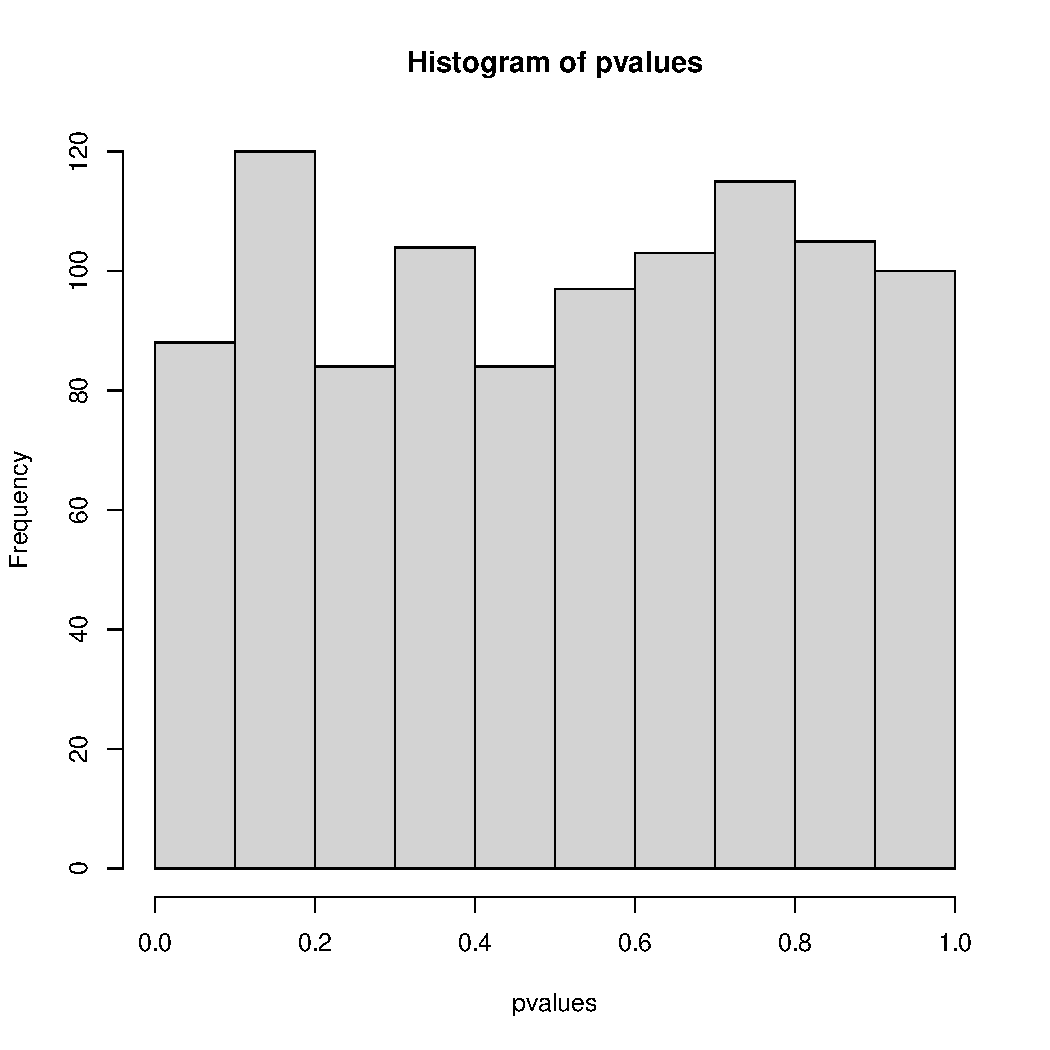
\includegraphics[width=\maxwidth]{figure/unnamed-chunk-7-1} 
\begin{kframe}\begin{alltt}
\hlkwd{sum}\hldef{(pvalues} \hlopt{<=} \hlnum{0.05}\hldef{)}
\end{alltt}
\begin{verbatim}
## [1] 49
\end{verbatim}
\end{kframe}
\end{knitrout}

Al realizar la suma de una lógica booleana, se coercia para que los valores falsos se conviertan en 0 y los verdaderos en 1. Así, al sumarlos, el resultado es numérico. 

En resumen, en este ejemplo hemos visto los siguientes objetos:
\begin{itemize}
\item Vectores: colección de uno o más datos del mismo tipo.
\item Matrices: conjunto de datos indexados por filas y columnas del mismo tipo. 
\item Arrays: generalización de una matriz que no tiene límite de dimensiones (pero debe tener una estructura rectangular). 
\item Data frames: estructura rectangular de dos dimensiones (filas y columnas) en la que cada columna puede ser de un tipo diferente. 
\item Listas: cajón desastre en el que se pueden meter muchas cosas de muchos tipos distintos. Muchas funciones devuelven listas u objetos que contienen listas.
\item Factores: vectores de un tipo especial (variable categórica).
\item Funciones: objetos que realizan una operación y devuelven algo. 
\end{itemize}

En el siguiente código se muestran las distintas maneras de acceder a una matriz. La indexación funciona [filas, columnas], y si un campo está sin rellenar implica todos sus datos.

\begin{knitrout}
\definecolor{shadecolor}{rgb}{0.969, 0.969, 0.969}\color{fgcolor}\begin{kframe}
\begin{alltt}
\hldef{randomdata[,} \hlnum{1}\hldef{]}
\hldef{randomdata[}\hlnum{2}\hldef{, ]}
\hldef{randomdata[,} \hlnum{2}\hldef{]}
\hldef{randomdata[}\hlnum{2}\hldef{,} \hlnum{3}\hldef{]}
\end{alltt}
\end{kframe}
\end{knitrout}

Al ejecutar la variable \code{class} creada anteriormente, no solo devuelve la lista de los elementos con las distintas etiquetas, si no que también muestra al final los distintos niveles. Como \code{factor} por detrás les asignó un valor entero que corresponda a la etiqueta dada, cuando se pide convertir en numérico, se devuelve el entero. La asignación de los valores se realiza por orden alfanumérico.

\begin{knitrout}
\definecolor{shadecolor}{rgb}{0.969, 0.969, 0.969}\color{fgcolor}\begin{kframe}
\begin{alltt}
\hldef{class}
\hlkwd{as.numeric}\hldef{(class)}
\end{alltt}
\end{kframe}
\end{knitrout}



\begin{knitrout}
\definecolor{shadecolor}{rgb}{0.969, 0.969, 0.969}\color{fgcolor}\begin{kframe}
\begin{alltt}
\hldef{pvalues[}\hlnum{1}\hldef{]}

\hlkwd{t.test}\hldef{(randomdata[}\hlnum{1}\hldef{, ]} \hlopt{~} \hldef{class)}

\hlkwd{t.test}\hldef{(randomdata[}\hlnum{1}\hldef{, ]} \hlopt{~} \hldef{class)}\hlopt{$}\hldef{p.value}

\hldef{pvalues[}\hlnum{1}\hlopt{:}\hlnum{10}\hldef{]} \hlopt{<} \hlnum{0.05}

\hlkwd{sum}\hldef{(}\hlkwd{c}\hldef{(}\hlnum{TRUE}\hldef{,} \hlnum{TRUE}\hldef{,} \hlnum{FALSE}\hldef{))}

\hlkwd{hist}\hldef{(}\hlkwd{c}\hldef{(}\hlnum{1}\hldef{,} \hlnum{2}\hldef{,} \hlnum{7}\hldef{,} \hlnum{7}\hldef{,} \hlnum{7}\hldef{,} \hlnum{8}\hldef{,} \hlnum{8}\hldef{))}
\end{alltt}
\end{kframe}
\end{knitrout}

\begin{knitrout}
\definecolor{shadecolor}{rgb}{0.969, 0.969, 0.969}\color{fgcolor}\begin{kframe}
\begin{alltt}
\hlcom{## For ease}
\hldef{rd2} \hlkwb{<-} \hldef{randomdata[}\hlnum{1}\hlopt{:}\hlnum{10}\hldef{, ]}

\hlcom{## Where we will store results}
\hldef{pv2} \hlkwb{<-} \hlkwd{vector}\hldef{(}\hlkwc{length} \hldef{=} \hlnum{10}\hldef{)}

\hlkwa{for}\hldef{(i} \hlkwa{in} \hlnum{1}\hlopt{:}\hlnum{10}\hldef{) \{}
    \hldef{pv2[i]} \hlkwb{<-} \hlkwd{t.test}\hldef{(rd2[i, ]} \hlopt{~} \hldef{class)}\hlopt{$}\hldef{p.value}
\hldef{\}}

\hldef{pv2}

\hlcom{## Compare with}
\hldef{pvalues[}\hlnum{1}\hlopt{:}\hlnum{10}\hldef{]}
\end{alltt}
\end{kframe}
\end{knitrout}

Ahora usamos apply. No lo hemos dicho explícitamente, pero cuando usamos apply estamos pasando una función (nuestra función anónima) a otra función. Esto es algo muy común y fácil en R: pasar funciones a otras funciones.
\begin{knitrout}
\definecolor{shadecolor}{rgb}{0.969, 0.969, 0.969}\color{fgcolor}\begin{kframe}
\begin{alltt}
\hlkwd{apply}\hldef{(rd2,} \hlnum{1}\hldef{,} \hlkwa{function}\hldef{(}\hlkwc{z}\hldef{)} \hlkwd{t.test}\hldef{(z} \hlopt{~} \hldef{class)}\hlopt{$}\hldef{p.value)}
\end{alltt}
\end{kframe}
\end{knitrout}

Esta es otra forma de hacerlo, pero es más verbosa (quizás incluso innecesariamente verbosa):

\begin{knitrout}
\definecolor{shadecolor}{rgb}{0.969, 0.969, 0.969}\color{fgcolor}\begin{kframe}
\begin{alltt}
\hldef{myfunction} \hlkwb{<-} \hlkwa{function}\hldef{(}\hlkwc{y}\hldef{,} \hlkwc{classfactor} \hldef{= class) \{}
    \hlkwd{t.test}\hldef{(y} \hlopt{~} \hldef{classfactor)}\hlopt{$}\hldef{p.value}
\hldef{\}}

\hlkwd{apply}\hldef{(rd2,} \hlnum{1}\hldef{, myfunction)}
\end{alltt}
\end{kframe}
\end{knitrout}

%14/10 - Ramón
\chapter{La consola de R para cálculos interactivos}
Independientemente de cómo interactuemos con R, una vez que iniciemos una sesión interactiva de R, siempre habrá una consola, que es donde podemos introducir comandos para que sean ejecutados por R. En RStudio, por ejemplo, la consola suele estar situada en la parte inferior izquierda.Todos los prompts en la consola empiezan con >.

\begin{knitrout}
\definecolor{shadecolor}{rgb}{0.969, 0.969, 0.969}\color{fgcolor}\begin{kframe}
\begin{alltt}
\hlnum{1} \hlopt{+} \hlnum{2}
\end{alltt}
\begin{verbatim}
## [1] 3
\end{verbatim}
\end{kframe}
\end{knitrout}

Mira la salida. En este documento, los trozos de código, si muestran salida, mostrarán la salida precedida por \#\#. En R (como en Python), \# es el carácter de comentario. En la consola, NO veremos el \#\# precediendo a la salida. Esto es sólo la forma en que está formateado en este documento (al igual que no se ve el > antes del comando). Fíjate también en que ves un [1], antes del 3. Esto se debe a que la salida de esa operación es, en realidad, un vector de longitud 1, y R está mostrando su índice. Aquí no ayuda mucho, pero lo haría si imprimiéramos 40 números:

\begin{knitrout}
\definecolor{shadecolor}{rgb}{0.969, 0.969, 0.969}\color{fgcolor}\begin{kframe}
\begin{alltt}
\hlnum{1}\hlopt{:}\hlnum{40}
\end{alltt}
\begin{verbatim}
##  [1]  1  2  3  4  5  6  7  8  9 10 11 12 13 14 15 16 17 18 19 20
## [21] 21 22 23 24 25 26 27 28 29 30 31 32 33 34 35 36 37 38 39 40
\end{verbatim}
\end{kframe}
\end{knitrout}

Se puede asignar 1 + 2 a una variable mediante <-. También se puede utilizar =, pero no se aconseja. Esto se debe a que se suele utilizar = cuando se pasan argumentos a una función, y utilizar la flecha permite diferenciar a simplevista las asignaciones. Para ver el valor de una variable, se puede escribir simplemente el nombre de la variable, utilizar print o hacer la asignación entre paréntesis (eso realiza la asignación y muestra el resultado por pantalla).

\begin{knitrout}
\definecolor{shadecolor}{rgb}{0.969, 0.969, 0.969}\color{fgcolor}\begin{kframe}
\begin{alltt}
\hldef{(v1} \hlkwb{<-} \hlnum{1} \hlopt{+} \hlnum{2}\hldef{)}
\end{alltt}
\begin{verbatim}
## [1] 3
\end{verbatim}
\begin{alltt}
\hlkwd{print}\hldef{(v1)}
\end{alltt}
\begin{verbatim}
## [1] 3
\end{verbatim}
\begin{alltt}
\hldef{v1}
\end{alltt}
\begin{verbatim}
## [1] 3
\end{verbatim}
\end{kframe}
\end{knitrout}

Se pueden separar dos comandos con un punto y coma (;), pero utilizarlo no suele ser una buena idea, solo en casos muy concretos. 

\begin{knitrout}
\definecolor{shadecolor}{rgb}{0.969, 0.969, 0.969}\color{fgcolor}\begin{kframe}
\begin{alltt}
\hldef{v1} \hlkwb{<-} \hlnum{1} \hlopt{+} \hlnum{2}\hldef{; v1}
\end{alltt}
\begin{verbatim}
## [1] 3
\end{verbatim}
\end{kframe}
\end{knitrout}

Es posible dividir comandos en varias líneas si R puede entender que la expresión no se ha terminado: 
\begin{verbatim}
v2 <-  4 - ( 3 * [Enter]
2)
\end{verbatim}

Cuando se hace esto, se ve un + que indica que la línea se continúa y que R sigue esperando más input. No obstante, hay ocasiones en las que esto puede ser confuso, y se puede cancelar mediante Ctrl + c en Linux o pulsando Escape para abortar la operación. 

Los paréntesis se ponen cuando el usuario opine que es apropiado y que facilite el entendimiento de una expresión. R utiliza las normas de precedencia usuales, pero en caso de duda, se pueden utilizar paréntesis.

\begin{knitrout}
\definecolor{shadecolor}{rgb}{0.969, 0.969, 0.969}\color{fgcolor}\begin{kframe}
\begin{alltt}
\hldef{v11} \hlkwb{<-} \hlnum{3} \hlopt{*} \hldef{(} \hlnum{5} \hlopt{+} \hlkwd{sqrt}\hldef{(}\hlnum{13}\hldef{)} \hlopt{-} \hlnum{3}\hlopt{^}\hldef{(}\hlnum{1}\hlopt{/}\hldef{(}\hlnum{4} \hlopt{+} \hlnum{1}\hldef{)))}
\end{alltt}
\end{kframe}
\end{knitrout}

\section{Nombrar variables}
Anteriormente hemos creado las variables \code{v1} y \code{v2}. Los nombres de las variables deben comenzar con una letra. También pueden empezar por un punto, pero entonces estarán ocultas. A continuación se pueden mezclar letras, números, puntos y barras bajas. Los nombres de las variables son case-sensitive, es decir, se diferencia entre las mayúsculas y minúsculas (v1 es diferente a V1). Una vez que se ha creado una variable, se puede utilizar la variable en lugar del contenido:

\begin{knitrout}
\definecolor{shadecolor}{rgb}{0.969, 0.969, 0.969}\color{fgcolor}\begin{kframe}
\begin{alltt}
\hldef{v3} \hlkwb{<-} \hlnum{5}
\hldef{(v4} \hlkwb{<-} \hldef{v1} \hlopt{+} \hldef{v3)}
\end{alltt}
\begin{verbatim}
## [1] 8
\end{verbatim}
\begin{alltt}
\hldef{(v5} \hlkwb{<-} \hldef{v1} \hlopt{*} \hldef{v3)}
\end{alltt}
\begin{verbatim}
## [1] 15
\end{verbatim}
\begin{alltt}
\hldef{(v6} \hlkwb{<-} \hldef{v1} \hlopt{/} \hldef{v3)}
\end{alltt}
\begin{verbatim}
## [1] 0.6
\end{verbatim}
\end{kframe}
\end{knitrout}

Las asignaciones posteriores sobreescriben las asignaciones previas.

\begin{knitrout}
\definecolor{shadecolor}{rgb}{0.969, 0.969, 0.969}\color{fgcolor}\begin{kframe}
\begin{alltt}
\hldef{(z2} \hlkwb{<-} \hlnum{33}\hldef{)}
\end{alltt}
\begin{verbatim}
## [1] 33
\end{verbatim}
\begin{alltt}
\hldef{z2} \hlkwb{<-} \hlnum{999}
\hldef{z2}
\end{alltt}
\begin{verbatim}
## [1] 999
\end{verbatim}
\begin{alltt}
\hldef{z2} \hlkwb{<-} \hlsng{"Now z2 is a sentence"}
\hldef{z2}
\end{alltt}
\begin{verbatim}
## [1] "Now z2 is a sentence"
\end{verbatim}
\end{kframe}
\end{knitrout}

Se puede borrar una variable de la siguiente forma:
\begin{knitrout}
\definecolor{shadecolor}{rgb}{0.969, 0.969, 0.969}\color{fgcolor}\begin{kframe}
\begin{alltt}
\hlkwd{rm}\hldef{(z2)}
\end{alltt}
\end{kframe}
\end{knitrout}

\section{Obtener ayuda}
Se puede acceder a la página de ayuda mediante:
\begin{knitrout}
\definecolor{shadecolor}{rgb}{0.969, 0.969, 0.969}\color{fgcolor}\begin{kframe}
\begin{alltt}
\hlkwd{help}\hldef{(mean)}
\end{alltt}
\end{kframe}
\end{knitrout}

También se puede utilizar la siguiente sintaxis:
\begin{knitrout}
\definecolor{shadecolor}{rgb}{0.969, 0.969, 0.969}\color{fgcolor}\begin{kframe}
\begin{alltt}
\hlopt{?}\hldef{mean}
\end{alltt}
\end{kframe}
\end{knitrout}

Hay otras formas de buscar ayuda sobre cómo hacer algo con R. Se puede buscar en Google, utilizar StackOverflow, etc. También hay un paquete \code{sos} que ayuda a buscar funciones y demás en paquetes que no están instalados, hacer un ranking de resultados de búsqueda, etc. A su vez, RStudio incluye un navegador de ayuda integrado. Todas las ayudas cuentan con una descripción de la función, los argumentos que admiten ( y su orden en caso de pasarlos sin nombre; en general es mejor añadir el nombre de cada parámetro a la hora de pasarlo) y el valor, es decir, lo que devuelve. En algunos casos se especifican las fuentes y referencias. También hay una sección de ejemplos de uso de la función.

Lo visto anteriormente proporciona información de funciones concretas. No obstante, hay veces que no sabemos exactamente cómo se llama la función que buscamos. Para ello, se puede utilizar las siguientes formas:
\begin{knitrout}
\definecolor{shadecolor}{rgb}{0.969, 0.969, 0.969}\color{fgcolor}\begin{kframe}
\begin{alltt}
\hlkwd{apropos}\hldef{(}\hlsng{"normal"}\hldef{)}
\end{alltt}
\begin{verbatim}
## [1] "normal_print"  "normalizePath"
\end{verbatim}
\begin{alltt}
\hlcom{# help.search("normal")}
\end{alltt}
\end{kframe}
\end{knitrout}

El comando \code{apropos} busca todos los paquetes que contengan en el nombre lo que se esté buscando. Por el contrario, \code{help.search} busca todos aquellos paquetes que, en la página de ayuda, tengan lo que se esté buscando. 

La función \code{args} devuelve los argumentos que se le puede pasar a una función.
\begin{knitrout}
\definecolor{shadecolor}{rgb}{0.969, 0.969, 0.969}\color{fgcolor}\begin{kframe}
\begin{alltt}
\hlkwd{args}\hldef{(rnorm)}
\end{alltt}
\begin{verbatim}
## function (n, mean = 0, sd = 1) 
## NULL
\end{verbatim}
\end{kframe}
\end{knitrout}

\section{Mensajes de error}
Los mensajes de error pueden ser un poco crípticos, pero en muchos casos leerlos ayuda a entender qué está pasando y cómo solucionar el problema. La mejor forma de parsear el mensaje de error es ir a la última línea que se ha ejecutado e ir ascendiendo para ver dónde puede estar el problema. A continuación se muestran algunos ejemplos de mensajes de errores:

\begin{knitrout}
\definecolor{shadecolor}{rgb}{0.969, 0.969, 0.969}\color{fgcolor}\begin{kframe}
\begin{alltt}
\hlkwd{apply}\hldef{(something,} \hlnum{1}\hldef{, mean)}
\end{alltt}


{\ttfamily\noindent\bfseries\color{errorcolor}{\#\# Error: objeto 'something' no encontrado}}\begin{alltt}
\hlkwd{apply}\hldef{(v3,} \hlnum{1}\hldef{, mean)} \hlcom{# en la ayuda se especifica qué es X}
\end{alltt}


{\ttfamily\noindent\bfseries\color{errorcolor}{\#\# Error in apply(v3, 1, mean): dim(X) debe tener una longitud positiva}}\begin{alltt}
\hlkwd{apply}\hldef{(F,} \hlnum{1}\hldef{, mean)}
\end{alltt}


{\ttfamily\noindent\bfseries\color{errorcolor}{\#\# Error in apply(F, 1, mean): dim(X) debe tener una longitud positiva}}\begin{alltt}
\hlkwd{log}\hldef{(}\hlsng{"23"}\hldef{)}
\end{alltt}


{\ttfamily\noindent\bfseries\color{errorcolor}{\#\# Error in log("{}23"{}): Argumento no numérico para una función matemática}}\begin{alltt}
\hlkwd{rnorm}\hldef{(}\hlsng{"a"}\hldef{)}
\end{alltt}


{\ttfamily\noindent\color{warningcolor}{\#\# Warning in rnorm("{}a"{}): NAs introducidos por coerción}}

{\ttfamily\noindent\bfseries\color{errorcolor}{\#\# Error in rnorm("{}a"{}): invalid arguments}}\begin{alltt}
\hlkwd{lug}\hldef{(}\hlnum{23}\hldef{)} \hlcom{# debería ser log}
\end{alltt}


{\ttfamily\noindent\bfseries\color{errorcolor}{\#\# Error in lug(23): no se pudo encontrar la función "{}lug"{}}}\begin{alltt}
\hlkwd{rnorm}\hldef{(}\hlnum{23}\hldef{,} \hlnum{1}\hldef{,} \hlnum{1}\hldef{,} \hlnum{1}\hldef{,} \hlnum{34}\hldef{)}
\end{alltt}


{\ttfamily\noindent\bfseries\color{errorcolor}{\#\# Error in rnorm(23, 1, 1, 1, 34): los argumentos no fueron usados (1, 34)}}\begin{alltt}
\hldef{x} \hlkwb{<-} \hlnum{1}\hlopt{:}\hlnum{10}
\hldef{y} \hlkwb{<-} \hlnum{11}\hlopt{:}\hlnum{21}
\hlkwd{plot}\hldef{(x, y)}
\end{alltt}


{\ttfamily\noindent\bfseries\color{errorcolor}{\#\# Error in xy.coords(x, y, xlabel, ylabel, log): 'x' and 'y' lengths differ}}\begin{alltt}
\hlkwd{lm}\hldef{(y} \hlopt{~} \hldef{x)}
\end{alltt}


{\ttfamily\noindent\bfseries\color{errorcolor}{\#\# Error in model.frame.default(formula = y \textasciitilde{} x, drop.unused.levels = TRUE): las longitudes variables difieren (encontradas para 'x')}}\begin{alltt}
\hldef{z} \hlkwb{<-} \hlnum{1}\hlopt{:}\hlnum{10}
\hlkwd{t.test}\hldef{(x} \hlopt{~} \hldef{z)}
\end{alltt}


{\ttfamily\noindent\bfseries\color{errorcolor}{\#\# Error in t.test.formula(x \textasciitilde{} z): grouping factor must have exactly 2 levels}}\end{kframe}
\end{knitrout}

En la consola, poniendo el nombre de la función, se puede acceder al código que realiza la función por detrás. Esto puede ser útil cuando la página de ayuda no sea suficiente para intentar localizar lo que intenta hacer la función y por qué falla.

\section{Estilo del código}
Aunque el código se escriba para la máquina, también debe ser legible por humanos, tanto uno mismo del futuro como otras personas. Por tanto, se recomienda no extenderse más allá de la columna 80 y utilizar espacios. Hay muchas guías de estilo de código, pero esas dos normas son las más básicas: si una línea de código es excesivamente larga, cuesta leerla entera al no poder verla completa a simple vista y tener que scrollear. 

Existe un paquete llamado \code{lintr} que permite corregir el estilo del código. 

Los comentarios también forman parte del estilo de código. Se suele separar la documentación para el usuario de la función (documentación de cabecera) de la documentación dentro del código que explica por qué se hacen algunas cosas.

\chapter{Leer datos en R y guardarlos desde R}
Hay muchas formas de cargar datos en R. Un ejemplo es \code{read.table} que sirve para todo tipo de datos, pero también hay algunos comandos más concretos como \code{read\_csv}.

\begin{knitrout}
\definecolor{shadecolor}{rgb}{0.969, 0.969, 0.969}\color{fgcolor}\begin{kframe}
\begin{alltt}
\hldef{X} \hlkwb{<-} \hlkwd{read.table}\hldef{(}\hlsng{"data/hit-table-500-text.txt"}\hldef{)}
\hlkwd{head}\hldef{(X)}
\hlcom{## We could save what we care about in variables with better names}
\hldef{align.length} \hlkwb{<-} \hldef{X[,} \hlnum{5}\hldef{]}
\hldef{score} \hlkwb{<-} \hldef{X[,} \hlnum{13}\hldef{]}
\hlkwd{summary}\hldef{(X)}
\end{alltt}
\end{kframe}
\end{knitrout}

El objeto no es una matriz, si no un data frame. Otro ejemplo sería el siguiente:
\begin{knitrout}
\definecolor{shadecolor}{rgb}{0.969, 0.969, 0.969}\color{fgcolor}\begin{kframe}
\begin{alltt}
\hldef{another.data.set} \hlkwb{<-} \hlkwd{read.table}\hldef{(}\hlsng{"data/AnotherDataSet.txt"}\hldef{,} \hlkwc{header} \hldef{=} \hlnum{TRUE}\hldef{)}
\hlkwd{summary}\hldef{(another.data.set)}
\end{alltt}
\begin{verbatim}
##       ID                 Age           Sex           
##  Length:5           Min.   :12.0   Length:5          
##  Class :character   1st Qu.:13.0   Class :character  
##  Mode  :character   Median :14.0   Mode  :character  
##                     Mean   :14.8                     
##                     3rd Qu.:16.0                     
##                     Max.   :19.0                     
##        Y        
##  Min.   :22.00  
##  1st Qu.:23.40  
##  Median :24.30  
##  Mean   :24.14  
##  3rd Qu.:25.00  
##  Max.   :26.00
\end{verbatim}
\end{kframe}
\end{knitrout}
Si se pone que no hay cabecera, parece que se lee lo mismo, pero en realidad hay algunas diferencias. Cuando se especifica que hay una cabecera, la primera línea con la descripción de las columnas no está numerada, mientras que cuando no se especifica, sí se numera y se considera como la primera fila, y esto es un error. R, por defecto, pone que cabecera es falso. Cuando no se sabe si un documento tiene o no cabecera, primero se carga el documento y luego se comprueba si el contenido se ha cargado bien. Por defecto, las columnas están separadas por espacios o tabuladores.

\section{Localización de ficheros}
Para que R pueda leer los ficheros, debe saber dónde buscarlos. Si los ficheros se encuentran en el directorio de trabajo, no hay ningún problema, ya que R los encuentra directamente. Para conocer el directorio de trabajo, se utiliza el comando \code{getwd()}. Si el fichero no se encuentra en el directorio de trabajo, hay varias opciones: proporcionar el path completo o mover el directorio de trabajo al lugar donde se encuentran los ficheros mediante \code{setwd()}. Para esto, es recomendable evitar en el nombre de directorios espacios, acentos y otros caracteres no ASCII.

\section{Missing values - NA}
Los missing values son algo muy común en estadística. Lo más sencillo es llamarlos como NA de not available. Otra forma es NaN, not a number. 

Puedes especificar el carácter que R debe interpretar como valor omitido, pero los dos procedimientos estándares son sustituir el valor como NA o sustituirlo por nada. Cuando haces cualquiera de los dos, en los datos que se leen deberías ver un NA. Lo mejor es, como de costumbre, ser explícito: utilizar un NA en sus datos originales, o utilizar alguna otra cadena de caracteres especiales para identificarlos. Lo más probable es que desees utilizar NA (o utilizar alguna otra combinación de caracteres y ser explícito), especialmente para las variables de carácter.

%16/10
Por defecto, R considera cualquier secuencia de blancos y tabuladores como separadores. Por tanto, si un missing value se representa con un espacio, sería necesario especificar el separador (por ejemplo, \code{sep = "\t"}) para que no dé error (al considerar R el espacio como parte del separador).

Al utilizar \code{summary}, en las columnas que sean de tipo int aparece un contador con las filas que contienen un NA. Sin embargo, esto no es así en las columnas cuyo contenido sea texto. Por tanto, no nos podemos fiar si summary no nos dice que no hay, hay que comprobar que efectivamente no haya. 

\section{Guardar tablas, datos y resultados}
Es posible guardar los datos en uan matriz o de forma tabular con \code{write.table}:
\begin{knitrout}
\definecolor{shadecolor}{rgb}{0.969, 0.969, 0.969}\color{fgcolor}\begin{kframe}
\begin{alltt}
\hlkwd{write.table}\hldef{(X,} \hlkwc{file} \hldef{=} \hlsng{"datos_guardados.txt"}\hldef{)}
\end{alltt}
\end{kframe}
\end{knitrout}

El problema que tiene esto es que en el documento de salida tiene una columna adicional que indica el número de línea, y se emplean los espacios como separadores. Todo esto se puede especificar mediante argumentos concretos en la función:

\begin{knitrout}
\definecolor{shadecolor}{rgb}{0.969, 0.969, 0.969}\color{fgcolor}\begin{kframe}
\begin{alltt}
\hlkwd{write.table}\hldef{(X,} \hlkwc{file} \hldef{=} \hlsng{"datos_guardados.txt"}\hldef{,} \hlkwc{sep} \hldef{=} \hlsng{"\textbackslash{}t"}\hldef{,}
            \hlkwc{quote} \hldef{=} \hlnum{FALSE}\hldef{,} \hlkwc{row.names} \hldef{=} \hlnum{FALSE}\hldef{)}
\end{alltt}
\end{kframe}
\end{knitrout}

En algunos casos, puede que los nombres de las filas sean importantes (por ejemplo, que sean el identificador). En ese caso, sería interesante guardar los nombres de las filas como columna en el dataframe:

\begin{knitrout}
\definecolor{shadecolor}{rgb}{0.969, 0.969, 0.969}\color{fgcolor}\begin{kframe}
\begin{alltt}
\hldef{X}\hlopt{$}\hldef{columna_nueva} \hlkwb{<-} \hlkwd{rownames}\hldef{(X)}
\end{alltt}
\end{kframe}
\end{knitrout}

\section{Guardar una sesión en R: .RData}
R permite guardar una imagen de la sesión actual en un fichero de extensión .RData. Esto se realiza mediante la función \code{save.image}:

\begin{knitrout}
\definecolor{shadecolor}{rgb}{0.969, 0.969, 0.969}\color{fgcolor}\begin{kframe}
\begin{alltt}
\hlkwd{save.image}\hldef{(}\hlkwc{file} \hldef{=} \hlsng{"this.RData"}\hldef{)}
\hlkwd{getwd}\hldef{()} \hlcom{#donde se guarda}
\end{alltt}
\end{kframe}
\end{knitrout}

Esta función guarda el entorno global, es decir, lo que se haya añadido por el usuario: variables, ficheros (incluso los ocultos), funciones, pero no los paquetes. También se guarda el estado del generador de números aleatorios si se ha utilizado. También existe la posibilidad de guardar un objeto concreto. Esto se logra mediante \code{save(datos-a-guardar, file = "datos-guardados.RData")}.

En una nueva terminal de R, se pueden cargar las imágenes (ya sea la total o de unos objetos concretos) con \code{load("datos-guardados.RData")}.

Por último, es posible utilizar \code{saveRDS} para guardar objetos individuales serializados (en binario) y \code{readRDS} para leerlos posteriormente. Sirve para un único objeto, pero permite poder asignarlo a un nombre que se decide al cargarlo.

\chapter{Scripts}
Mantener todo el código en uno o varios scripts y ejecutarlo directamente desde el script y no desde la consola tiene varias ventajas:
\begin{itemize}
\item Permite mantener un registro de todo lo que se ha hecho y tenerlo organizado, con comentarios, etc.
\item Permite realizar cálculos no interactivos. Por ejemplo, ejecutar un análisis muy largo o volver a ejecutar todo el análisis y los gráficos sin querer.
\end{itemize}

\section{Utilizar un script}
Hay dos maneras básicas de utilizar un script:
\begin{itemize}
\item De forma interactiva; lo que se ha hecho hasta entonces. Por ejemplo, RStudio permite seleccionar una parte del código y lanzarlo al intérprete de R, ejecutándolo desde la consola.
\item De forma no interactiva:
\begin{itemize}
\item Utilizando \code{source("script.R")}. En la sesión de R en la que se haya puesto esto, se importan las variables, funciones (y todo) del script. La diferencia es que, como es no interactivo, si se llaman a funciones (como por ejemplo, \code{mean(x)}), no se muestra el resultado por pantalla; para ello sería necesario utilizar print. 
\item Desde la shell. Esto tiene la ventaja de no tener que mantener una ventana abierta con R hasta que el código finalice, por lo que es muy cómodo para los trabajos muy largos. La forma preferida es:

\verb@ R --vanilla < script1.R > script1.Rout @

La opción de vanilla permite que la sesión sea lo más reproducible posible, es decir, sin cargar librerías adicionales, sesiones de R anteriores, etc. Otra manera muy similar es \verb@ R --vanilla -f script1.R > script1.Rout @ Con esto lo que conseguimos es que el resultado del script1 se guarde directamente en otro fichero. 
\end{itemize}
\end{itemize}

\chapter{Estructuras de datos básicas en R}
\section{Vectores}
Los vectores son la estructura de datos más simple de R. Guardan una serie de objetos del mismo tipo, uno detrás de otro, en una sola dimensión.

\begin{knitrout}
\definecolor{shadecolor}{rgb}{0.969, 0.969, 0.969}\color{fgcolor}\begin{kframe}
\begin{alltt}
\hldef{v1} \hlkwb{<-} \hlkwd{c}\hldef{(}\hlnum{1}\hldef{,} \hlnum{2}\hldef{,} \hlnum{3}\hldef{)} \hlcom{#vector de números enteros }
\hlcom{#               (se guardan como floats si no se fuerza)}
\hldef{v2} \hlkwb{<-} \hlkwd{c}\hldef{(}\hlsng{"a"}\hldef{,} \hlsng{"b"}\hldef{,} \hlsng{"cucu"}\hldef{)} \hlcom{#vector de strings}
\hldef{v3} \hlkwb{<-} \hlkwd{c}\hldef{(}\hlnum{1.9}\hldef{,} \hlnum{2.5}\hldef{,} \hlnum{0.6}\hldef{)} \hlcom{#vector de números float}
\hldef{v4} \hlkwb{<-} \hlkwd{c}\hldef{(}\hlnum{4}\hldef{,} \hlsng{"a"}\hldef{)} \hlcom{#convierte el 4 en "4"}
\end{alltt}
\end{kframe}
\end{knitrout}

La \code{c} viene de concatenar, ya que hace precisamente eso: concatena lo que se le ponga a continuación. 

Muchas funciones operan directamente en vectores enteros sin necesidad de realizar un loop sobre cada uno de los objetos en él:
\begin{knitrout}
\definecolor{shadecolor}{rgb}{0.969, 0.969, 0.969}\color{fgcolor}\begin{kframe}
\begin{alltt}
\hlkwd{log}\hldef{(v1)}
\end{alltt}
\begin{verbatim}
## [1] 0.0000000 0.6931472 1.0986123
\end{verbatim}
\begin{alltt}
\hlkwd{exp}\hldef{(v3)}
\end{alltt}
\begin{verbatim}
## [1]  6.685894 12.182494  1.822119
\end{verbatim}
\begin{alltt}
\hlnum{2} \hlopt{*} \hldef{v1}
\end{alltt}
\begin{verbatim}
## [1] 2 4 6
\end{verbatim}
\begin{alltt}
\hldef{v3}\hlopt{/}\hlnum{0.7}
\end{alltt}
\begin{verbatim}
## [1] 2.7142857 3.5714286 0.8571429
\end{verbatim}
\end{kframe}
\end{knitrout}

\subsection{Funciones para crear vectores}
Se pueden crear vectores concatenando elementos, pero hay otras dos funciones para crearlos que tienen algo de estructura: \code{seq} (de secuencia) y \code{rep} (de repetición). La función \code{seq} tiene cuatro formas de invocación:
\begin{knitrout}
\definecolor{shadecolor}{rgb}{0.969, 0.969, 0.969}\color{fgcolor}\begin{kframe}
\begin{alltt}
\hlkwd{seq}\hldef{(}\hlkwc{from} \hldef{=} \hlnum{1}\hldef{,} \hlkwc{to} \hldef{=} \hlnum{10}\hldef{)}
\end{alltt}
\begin{verbatim}
##  [1]  1  2  3  4  5  6  7  8  9 10
\end{verbatim}
\begin{alltt}
\hlkwd{seq}\hldef{(}\hlkwc{from} \hldef{=} \hlnum{1}\hldef{,} \hlkwc{to} \hldef{=} \hlnum{10}\hldef{,} \hlkwc{by} \hldef{=} \hlnum{2}\hldef{)}
\end{alltt}
\begin{verbatim}
## [1] 1 3 5 7 9
\end{verbatim}
\begin{alltt}
\hlkwd{seq}\hldef{(}\hlkwc{from} \hldef{=} \hlnum{1}\hldef{,} \hlkwc{to} \hldef{=} \hlnum{10}\hldef{,} \hlkwc{length.out} \hldef{=} \hlnum{3}\hldef{)}
\end{alltt}
\begin{verbatim}
## [1]  1.0  5.5 10.0
\end{verbatim}
\begin{alltt}
\hlnum{1}\hlopt{:}\hlnum{5}
\end{alltt}
\begin{verbatim}
## [1] 1 2 3 4 5
\end{verbatim}
\end{kframe}
\end{knitrout}

\code{rep} también tiene varias invocaciones comunes:
\begin{knitrout}
\definecolor{shadecolor}{rgb}{0.969, 0.969, 0.969}\color{fgcolor}\begin{kframe}
\begin{alltt}
\hlkwd{rep}\hldef{(}\hlnum{2}\hldef{,} \hlnum{5}\hldef{)}
\end{alltt}
\begin{verbatim}
## [1] 2 2 2 2 2
\end{verbatim}
\begin{alltt}
\hlkwd{rep}\hldef{(}\hlnum{1}\hlopt{:}\hlnum{3}\hldef{,} \hlnum{2}\hldef{)}
\end{alltt}
\begin{verbatim}
## [1] 1 2 3 1 2 3
\end{verbatim}
\begin{alltt}
\hlkwd{rep}\hldef{(}\hlnum{1}\hlopt{:}\hlnum{3}\hldef{,} \hlnum{2}\hlopt{:}\hlnum{4}\hldef{)}
\end{alltt}
\begin{verbatim}
## [1] 1 1 2 2 2 3 3 3 3
\end{verbatim}
\end{kframe}
\end{knitrout}

En este caso, es importante que el segundo argumento de \code{rep} sea un único valor (y repita todos los elementos del primer argumento las veces indicadas) o un conjunto de valores de las mismas dimensiones que el primer argumento (y se asigne a cada valor su respectivo número de repetición). 

\section{Crear vectores a partir de otros vectores}
Se pueden concatenar dos vectores:

\begin{knitrout}
\definecolor{shadecolor}{rgb}{0.969, 0.969, 0.969}\color{fgcolor}\begin{kframe}
\begin{alltt}
\hldef{v1} \hlkwb{<-} \hlnum{1}\hlopt{:}\hlnum{4}
\hldef{v2} \hlkwb{<-} \hlnum{7}\hlopt{:}\hlnum{12}
\hldef{(v3} \hlkwb{<-} \hlkwd{c}\hldef{(v1, v2))}
\end{alltt}
\begin{verbatim}
##  [1]  1  2  3  4  7  8  9 10 11 12
\end{verbatim}
\end{kframe}
\end{knitrout}

Si se emplean operaciones aritméticas en vectores que no son de la misma longitud, se utiliza la \textbf{regla de reciclaje}, es decir, se reutiliza el vector más pequeño cuando llega a su fin las veces necesarias hasta haber terminado las operaciones con el vector grande:

\begin{knitrout}
\definecolor{shadecolor}{rgb}{0.969, 0.969, 0.969}\color{fgcolor}\begin{kframe}
\begin{alltt}
\hldef{v1} \hlkwb{<-} \hlnum{1}\hlopt{:}\hlnum{3}
\hldef{v2} \hlkwb{<-} \hlnum{11}\hlopt{:}\hlnum{12}
\hldef{v1} \hlopt{+} \hldef{v2}
\end{alltt}


{\ttfamily\noindent\color{warningcolor}{\#\# Warning in v1 + v2: longitud de objeto mayor no es múltiplo de la longitud de uno menor}}\begin{verbatim}
## [1] 12 14 14
\end{verbatim}
\end{kframe}
\end{knitrout}

%21/10 - Ramón
En ocasiones se produce un warning que avisa sobre la reutilización de uno de los vectores. Sin embargo, esto no ocurre siempre, ua que el warning se suprime cuando el vector a reutilizar se repite una ronda concreta (y no se quede a medias durante el reciclaje).

\section{Logical operations}
Se pueden comparar los elementos de un vector con algo para obtener un vector de elementos lógicos TRUE y FALSE. Esto es común en varios lenguajes de programación, pero hay que tener en cuenta la diferencia entre \code{|} y \code{||} y entre \code{\&\&} y \code{\&}. También se puede usar \code{xor} para obtener TRUE cuando solo uno de las condiciones es verdadera (no ambas).

\begin{knitrout}
\definecolor{shadecolor}{rgb}{0.969, 0.969, 0.969}\color{fgcolor}\begin{kframe}
\begin{alltt}
\hldef{v1} \hlkwb{<-} \hlnum{1}\hlopt{:}\hlnum{5}
\hldef{v1} \hlopt{<} \hlnum{3}
\end{alltt}
\begin{verbatim}
## [1]  TRUE  TRUE FALSE FALSE FALSE
\end{verbatim}
\begin{alltt}
\hldef{(v2} \hlkwb{<-} \hldef{(v1} \hlopt{<} \hlnum{3}\hldef{))}
\end{alltt}
\begin{verbatim}
## [1]  TRUE  TRUE FALSE FALSE FALSE
\end{verbatim}
\begin{alltt}
\hldef{v11} \hlkwb{<-} \hlkwd{c}\hldef{(}\hlnum{1}\hldef{,} \hlnum{1}\hldef{,} \hlnum{3}\hldef{,} \hlnum{5}\hldef{,} \hlnum{4}\hldef{)}
\hldef{v1} \hlopt{==} \hldef{v11}
\end{alltt}
\begin{verbatim}
## [1]  TRUE FALSE  TRUE FALSE FALSE
\end{verbatim}
\begin{alltt}
\hldef{v1} \hlopt{!=} \hldef{v11}
\end{alltt}
\begin{verbatim}
## [1] FALSE  TRUE FALSE  TRUE  TRUE
\end{verbatim}
\begin{alltt}
\hlopt{!}\hldef{(v1} \hlopt{==} \hldef{v11)}
\end{alltt}
\begin{verbatim}
## [1] FALSE  TRUE FALSE  TRUE  TRUE
\end{verbatim}
\begin{alltt}
\hlkwd{identical}\hldef{(v1, v11)}
\end{alltt}
\begin{verbatim}
## [1] FALSE
\end{verbatim}
\begin{alltt}
\hldef{v3} \hlkwb{<-} \hlkwd{c}\hldef{(}\hlnum{TRUE}\hldef{,} \hlnum{FALSE}\hldef{,} \hlnum{TRUE}\hldef{,} \hlnum{FALSE}\hldef{,} \hlnum{TRUE}\hldef{)}
\hlopt{!}\hldef{v3}
\end{alltt}
\begin{verbatim}
## [1] FALSE  TRUE FALSE  TRUE FALSE
\end{verbatim}
\begin{alltt}
\hldef{v2} \hlopt{&} \hldef{v3}
\end{alltt}
\begin{verbatim}
## [1]  TRUE FALSE FALSE FALSE FALSE
\end{verbatim}
\begin{alltt}
\hldef{v2} \hlopt{|} \hldef{v3}
\end{alltt}
\begin{verbatim}
## [1]  TRUE  TRUE  TRUE FALSE  TRUE
\end{verbatim}
\begin{alltt}
\hldef{(v1} \hlopt{>} \hlnum{3}\hldef{)} \hlopt{&} \hldef{(v11} \hlopt{>=} \hlnum{2}\hldef{)}
\end{alltt}
\begin{verbatim}
## [1] FALSE FALSE FALSE  TRUE  TRUE
\end{verbatim}
\begin{alltt}
\hldef{(v1} \hlopt{>} \hlnum{3}\hldef{)} \hlopt{|} \hldef{(v11} \hlopt{>=} \hlnum{2}\hldef{)}
\end{alltt}
\begin{verbatim}
## [1] FALSE FALSE  TRUE  TRUE  TRUE
\end{verbatim}
\begin{alltt}
\hlkwd{xor}\hldef{(v2, v3)}
\end{alltt}
\begin{verbatim}
## [1] FALSE  TRUE  TRUE FALSE  TRUE
\end{verbatim}
\end{kframe}
\end{knitrout}

\subsection{Valores lógicos 0 y 1}
En R, al igual que en otros lenguajes de programación, se pueden utilizar valores lógicos como si fuesen numéricos: se puede tratar \code{TRUE} como 1 y \code{FALSE} como 0. Además, \code{TRUE} puede ser cualquier otro número diferente a 0. 

El operador \code{which} opera en un vector lógico, no en el vector directamente, y devuelve las posiciones que son verdaderas. \code{length} cuenta la longitud de la salida:

\begin{knitrout}
\definecolor{shadecolor}{rgb}{0.969, 0.969, 0.969}\color{fgcolor}\begin{kframe}
\begin{alltt}
\hldef{vv} \hlkwb{<-} \hlkwd{c}\hldef{(}\hlnum{1}\hldef{,} \hlnum{3}\hldef{,} \hlnum{10}\hldef{,} \hlnum{2}\hldef{,} \hlnum{9}\hldef{,} \hlnum{5}\hldef{,} \hlnum{4}\hldef{,} \hlnum{6}\hlopt{:}\hlnum{8}\hldef{)}
\hlkwd{length}\hldef{(}\hlkwd{which}\hldef{(vv} \hlopt{<} \hlnum{5}\hldef{))}
\end{alltt}
\begin{verbatim}
## [1] 4
\end{verbatim}
\end{kframe}
\end{knitrout}

Es importante remarcar no utilizar T para TRUE y F para FALSE, aunque se pueda hacer. Esto se debe a que se puede redefinir el valor de T y F a que no correspondan a TRUE y FALSE (lo cual es muy difícil de debuggear), mientras que TRUE y FALSE siempre significarán lo mismo al no poder redefinirse. 

\subsection{Cortocircuito de operaciones lógicas}
Los operadores \code{\&\&} y \code{||} son cortocircuitos. Los dobles caracteres evalúan el segundo elemento sólo si la evaluación del primero no permite saber el resultado de la operación. Cuando se va a hacer un and y la primera condición es FALSE, no hace falta evaluar la segunda condición, ya que se conoce el resultado (de igual forma si en un or la primera condición es TRUE). Así, esto se puede utilizar para condicionar la ejecución de la segunda condición:

\begin{knitrout}
\definecolor{shadecolor}{rgb}{0.969, 0.969, 0.969}\color{fgcolor}\begin{kframe}
\begin{alltt}
\hldef{a} \hlkwb{<-} \hlsng{"hola"}
\hlkwa{if} \hldef{(}\hlkwd{is.numeric}\hldef{(a)} \hlopt{&&} \hlkwd{log}\hldef{(a))} \hlkwd{cat}\hldef{(}\hlsng{"\textbackslash{}n we entered in the if"}\hldef{)}
\end{alltt}
\end{kframe}
\end{knitrout}

En el ejemplo anterior, sólo se quiere evaluar el logaritmo de un número. Por ello, con \&\&, primero se evalúa si la variable es un número y, en caso afirmativo, se ejecuta el logaritmo. En caso de que la variable no sea numérica (como es el caso del ejemplo), utilizar un solo \& resultaría en un error, y no sería lo que nos interesa. 

\begin{knitrout}
\definecolor{shadecolor}{rgb}{0.969, 0.969, 0.969}\color{fgcolor}\begin{kframe}
\begin{alltt}
\hldef{a1} \hlkwb{<-} \hlkwd{c}\hldef{(}\hlnum{TRUE}\hldef{,} \hlnum{FALSE}\hldef{)}
\hldef{b1} \hlkwb{<-} \hlkwd{c}\hldef{(}\hlnum{TRUE}\hldef{,} \hlnum{TRUE}\hldef{)}

\hldef{a1} \hlopt{&&} \hldef{b1}
\end{alltt}


{\ttfamily\noindent\bfseries\color{errorcolor}{\#\# Error in a1 \&\& b1: 'length = 2' in coercion to 'logical(1)'}}\begin{alltt}
\hldef{a1} \hlopt{||} \hldef{b1}
\end{alltt}


{\ttfamily\noindent\bfseries\color{errorcolor}{\#\# Error in a1 || b1: 'length = 2' in coercion to 'logical(1)'}}\end{kframe}
\end{knitrout}

Hay que tener en cuenta que no se deben utilizar vectores con más de un elemento con cortocircuitos, ya que sólo se evalúa el primer valor. 

\section{Nombres de elementos}
Los elementos de un vector pueden tener nombres (que deben ser únicos). Esto permite acceder a los vectores utilizando nombres en lugar de posiciones, lo que puede ser más intuitivo. 

\begin{knitrout}
\definecolor{shadecolor}{rgb}{0.969, 0.969, 0.969}\color{fgcolor}\begin{kframe}
\begin{alltt}
\hldef{ages} \hlkwb{<-} \hlkwd{c}\hldef{(}\hlkwc{Juan} \hldef{=} \hlnum{23}\hldef{,} \hlkwc{Maria} \hldef{=} \hlnum{35}\hldef{,} \hlkwc{Irene} \hldef{=} \hlnum{12}\hldef{,} \hlkwc{Ana} \hldef{=} \hlnum{93}\hldef{)}
\hlkwd{names}\hldef{(ages)}
\end{alltt}
\begin{verbatim}
## [1] "Juan"  "Maria" "Irene" "Ana"
\end{verbatim}
\begin{alltt}
\hldef{ages}
\end{alltt}
\begin{verbatim}
##  Juan Maria Irene   Ana 
##    23    35    12    93
\end{verbatim}
\begin{alltt}
\hldef{ages[}\hlsng{"Juan"}\hldef{]}
\end{alltt}
\begin{verbatim}
## Juan 
##   23
\end{verbatim}
\end{kframe}
\end{knitrout}

\section{Acceder y modificar elementos de un vector: indexación y subsetting}
\subsection{Indexación de vectores}
Hay cuatro formas para acceder a elementos específicos de un vector:
\begin{itemize}
\item Especificando las posiciones: mediante índices
\item Dando los nombres de los elementos
\item Utilizando un vector lógico
\item Utilizando cualquier expresión que genere cualquiera de las anteriores.
\end{itemize}
Las posiciones y nombres se dan entre corchetes ([]).

Especificando las posiciones deseadas:
\begin{knitrout}
\definecolor{shadecolor}{rgb}{0.969, 0.969, 0.969}\color{fgcolor}\begin{kframe}
\begin{alltt}
\hldef{(w} \hlkwb{<-} \hlnum{9}\hlopt{:}\hlnum{18}\hldef{)}
\end{alltt}
\begin{verbatim}
##  [1]  9 10 11 12 13 14 15 16 17 18
\end{verbatim}
\begin{alltt}
\hldef{w[}\hlnum{1}\hldef{]}
\end{alltt}
\begin{verbatim}
## [1] 9
\end{verbatim}
\begin{alltt}
\hldef{w[}\hlnum{2}\hldef{]}
\end{alltt}
\begin{verbatim}
## [1] 10
\end{verbatim}
\begin{alltt}
\hldef{w[}\hlkwd{c}\hldef{(}\hlnum{4}\hldef{,} \hlnum{3}\hldef{,} \hlnum{2}\hldef{)]}
\end{alltt}
\begin{verbatim}
## [1] 12 11 10
\end{verbatim}
\end{kframe}
\end{knitrout}

\begin{knitrout}
\definecolor{shadecolor}{rgb}{0.969, 0.969, 0.969}\color{fgcolor}\begin{kframe}
\begin{alltt}
\hldef{w[}\hlkwd{c}\hldef{(}\hlnum{1}\hldef{,} \hlnum{3}\hldef{)]} \hlcom{## not the same as}
\end{alltt}
\begin{verbatim}
## [1]  9 11
\end{verbatim}
\begin{alltt}
\hldef{w[}\hlkwd{c}\hldef{(}\hlnum{3}\hldef{,} \hlnum{1}\hldef{)]}
\end{alltt}
\begin{verbatim}
## [1] 11  9
\end{verbatim}
\end{kframe}
\end{knitrout}

\begin{knitrout}
\definecolor{shadecolor}{rgb}{0.969, 0.969, 0.969}\color{fgcolor}\begin{kframe}
\begin{alltt}
\hldef{w[}\hlnum{1}\hlopt{:}\hlnum{2}\hldef{]}
\end{alltt}
\begin{verbatim}
## [1]  9 10
\end{verbatim}
\begin{alltt}
\hldef{w[}\hlnum{3}\hlopt{:}\hlnum{6}\hldef{]}
\end{alltt}
\begin{verbatim}
## [1] 11 12 13 14
\end{verbatim}
\begin{alltt}
\hldef{w[}\hlkwd{seq}\hldef{(}\hlnum{1}\hldef{,} \hlnum{8}\hldef{,} \hlkwc{by} \hldef{=} \hlnum{3}\hldef{)]}
\end{alltt}
\begin{verbatim}
## [1]  9 12 15
\end{verbatim}
\begin{alltt}
\hldef{vv} \hlkwb{<-} \hlkwd{seq}\hldef{(}\hlnum{1}\hldef{,} \hlnum{8}\hldef{,} \hlkwc{by} \hldef{=} \hlnum{3}\hldef{)}
\hldef{w[vv]}
\end{alltt}
\begin{verbatim}
## [1]  9 12 15
\end{verbatim}
\end{kframe}
\end{knitrout}


Especificando las posiciones que no se desean (el vector original no se modifica):
\begin{knitrout}
\definecolor{shadecolor}{rgb}{0.969, 0.969, 0.969}\color{fgcolor}\begin{kframe}
\begin{alltt}
\hldef{w[}\hlopt{-}\hlnum{1}\hldef{]}
\end{alltt}
\begin{verbatim}
## [1] 10 11 12 13 14 15 16 17 18
\end{verbatim}
\begin{alltt}
\hldef{w[}\hlopt{-}\hlkwd{c}\hldef{(}\hlnum{1}\hldef{,} \hlnum{3}\hldef{)]} \hlcom{## of course, the same as following}
\end{alltt}
\begin{verbatim}
## [1] 10 12 13 14 15 16 17 18
\end{verbatim}
\begin{alltt}
\hldef{w[}\hlopt{-}\hlkwd{c}\hldef{(}\hlnum{3}\hldef{,} \hlnum{1}\hldef{)]}
\end{alltt}
\begin{verbatim}
## [1] 10 12 13 14 15 16 17 18
\end{verbatim}
\end{kframe}
\end{knitrout}


Utilizando nombres
\begin{knitrout}
\definecolor{shadecolor}{rgb}{0.969, 0.969, 0.969}\color{fgcolor}\begin{kframe}
\begin{alltt}
\hldef{ages} \hlkwb{<-} \hlkwd{c}\hldef{(}\hlkwc{Juan} \hldef{=} \hlnum{23}\hldef{,} \hlkwc{Maria} \hldef{=} \hlnum{35}\hldef{,} \hlkwc{Irene} \hldef{=} \hlnum{12}\hldef{,} \hlkwc{Ana} \hldef{=} \hlnum{93}\hldef{)}
\hldef{ages[}\hlsng{"Irene"}\hldef{]}
\end{alltt}
\begin{verbatim}
## Irene 
##    12
\end{verbatim}
\begin{alltt}
\hldef{ages[}\hlkwd{c}\hldef{(}\hlsng{"Irene"}\hldef{,} \hlsng{"Juan"}\hldef{,} \hlsng{"Irene"}\hldef{)]}
\end{alltt}
\begin{verbatim}
## Irene  Juan Irene 
##    12    23    12
\end{verbatim}
\end{kframe}
\end{knitrout}


Utilizando un vector lógico \ldots
\begin{knitrout}
\definecolor{shadecolor}{rgb}{0.969, 0.969, 0.969}\color{fgcolor}\begin{kframe}
\begin{alltt}
\hldef{ages[}\hlkwd{c}\hldef{(}\hlnum{FALSE}\hldef{,} \hlnum{TRUE}\hldef{,} \hlnum{TRUE}\hldef{,} \hlnum{FALSE}\hldef{)]}
\end{alltt}
\begin{verbatim}
## Maria Irene 
##    35    12
\end{verbatim}
\begin{alltt}
\hlcom{## what are thes doing? Avoid these things}
\hldef{ages[}\hlkwd{c}\hldef{(}\hlnum{FALSE}\hldef{,} \hlnum{TRUE}\hldef{)]}
\end{alltt}
\begin{verbatim}
## Maria   Ana 
##    35    93
\end{verbatim}
\begin{alltt}
\hldef{ages[}\hlkwd{c}\hldef{(}\hlnum{TRUE}\hldef{,} \hlnum{TRUE}\hldef{,} \hlnum{FALSE}\hldef{)]}
\end{alltt}
\begin{verbatim}
##  Juan Maria   Ana 
##    23    35    93
\end{verbatim}
\end{kframe}
\end{knitrout}

\ldots o algo que es un vector lógico implícito 
\begin{knitrout}
\definecolor{shadecolor}{rgb}{0.969, 0.969, 0.969}\color{fgcolor}\begin{kframe}
\begin{alltt}
\hlcom{## All less than 12}
\hldef{w[w} \hlopt{<} \hlnum{12}\hldef{]}
\end{alltt}
\begin{verbatim}
## [1]  9 10 11
\end{verbatim}
\begin{alltt}
\hlcom{## same, but more confusing (here, not always)}
\hldef{w[}\hlopt{!}\hldef{(w} \hlopt{>=} \hlnum{12}\hldef{)]}
\end{alltt}
\begin{verbatim}
## [1]  9 10 11
\end{verbatim}
\begin{alltt}
\hlcom{## All less than the median}
\hldef{w[w} \hlopt{<} \hlkwd{median}\hldef{(w)]}
\end{alltt}
\begin{verbatim}
## [1]  9 10 11 12 13
\end{verbatim}
\end{kframe}
\end{knitrout}


Si se puede acceder, también se puede modificar: 
\begin{knitrout}
\definecolor{shadecolor}{rgb}{0.969, 0.969, 0.969}\color{fgcolor}\begin{kframe}
\begin{alltt}
\hldef{ages[}\hlsng{"Irene"}\hldef{]} \hlkwb{<-} \hlnum{19}
\hldef{ages}
\end{alltt}
\begin{verbatim}
##  Juan Maria Irene   Ana 
##    23    35    19    93
\end{verbatim}
\begin{alltt}
\hldef{w[}\hlnum{1}\hldef{]} \hlkwb{<-} \hlnum{9999}
\hldef{w}
\end{alltt}
\begin{verbatim}
##  [1] 9999   10   11   12   13   14   15   16   17   18
\end{verbatim}
\begin{alltt}
\hldef{w[vv]} \hlkwb{<-} \hlnum{103}
\hldef{w}
\end{alltt}
\begin{verbatim}
##  [1] 103  10  11 103  13  14 103  16  17  18
\end{verbatim}
\end{kframe}
\end{knitrout}


Pero compara esto:
\begin{knitrout}
\definecolor{shadecolor}{rgb}{0.969, 0.969, 0.969}\color{fgcolor}\begin{kframe}
\begin{alltt}
\hldef{w[]} \hlkwb{<-} \hlnum{77}
\hldef{w[]} \hlkwb{<-} \hlnum{17}\hlopt{:}\hlnum{55}
\end{alltt}


{\ttfamily\noindent\color{warningcolor}{\#\# Warning in w[] <- 17:55: número de elementos para sustituir no es un múltiplo de la longitud del reemplazo}}\begin{alltt}
\hldef{w} \hlkwb{<-} \hlnum{17}\hlopt{:}\hlnum{55}
\end{alltt}
\end{kframe}
\end{knitrout}


\section{Interludio: comparación de floats}
Comparar valores numéricos muy similares puede ser complicado y muy delicado debido al redondeo y algunos números que no se pueden representar exactamente en notación binaria. De forma predeterminada, R muestra 7 dígitos significativos.

\begin{knitrout}
\definecolor{shadecolor}{rgb}{0.969, 0.969, 0.969}\color{fgcolor}\begin{kframe}
\begin{alltt}
\hldef{x}  \hlkwb{<-}  \hlnum{1.999999}
\hldef{x}
\end{alltt}
\begin{verbatim}
## [1] 1.999999
\end{verbatim}
\begin{alltt}
\hldef{x} \hlopt{-} \hlnum{2}
\end{alltt}
\begin{verbatim}
## [1] -1e-06
\end{verbatim}
\begin{alltt}
\hldef{x} \hlkwb{<-} \hlnum{1.9999999999999}
\hldef{x}
\end{alltt}
\begin{verbatim}
## [1] 2
\end{verbatim}
\begin{alltt}
\hldef{x}\hlopt{-}\hlnum{2}
\end{alltt}
\begin{verbatim}
## [1] -9.992007e-14
\end{verbatim}
\end{kframe}
\end{knitrout}

Todos los dígitos están presentes, pero en el segundo caso, no se muestran. Además, \code{x-2} no es exactamente $-1 \times 10^{-13}$. En R se suelen redondear los números con una precisión de 53 dígitos binarios, por lo que dos números decimales no serán iguales de forma diable a menos que hayan sido calculados por el mismo algoritmo, y ni siquiera entonces: 
\begin{verbatim}
a <- sqrt(2)
a * a == 2
[1] FALSE
a * a - 2
[1] 4.440892e-16
\end{verbatim}

Otro ejemplo:
\begin{knitrout}
\definecolor{shadecolor}{rgb}{0.969, 0.969, 0.969}\color{fgcolor}\begin{kframe}
\begin{alltt}
\hlnum{0.1} \hlopt{+} \hlnum{0.2} \hlopt{==} \hlnum{0.3}
\end{alltt}
\begin{verbatim}
## [1] FALSE
\end{verbatim}
\begin{alltt}
\hldef{(}\hlnum{0.1} \hlopt{+} \hlnum{0.2}\hldef{)} \hlopt{-} \hlnum{0.3}
\end{alltt}
\begin{verbatim}
## [1] 5.551115e-17
\end{verbatim}
\end{kframe}
\end{knitrout}

En resumen: desconfía extremadamente siempre que veas una comparación de igualdad de dos números en coma flotante; es poco probable que haga lo que quieres. Si sabes lo que estás haciendo, echa un vistazo a \code{all.equal} para comparaciones de igualdad de objetos casi iguales.

\section{Factores}
Los factores son unos tipos especiales de vectores. Los necesitamos para diferenciar entre un vector de caracteres y un vector que representa variables categóricas. El vector \code{char.vec <- c("abc", "de", "fghi")} contiene varias cadenas de caracteres. Supongamos ahora que tenemos un estudio en el que registramos el sexo de los participantes. Cuando analizamos los datos queremos que R sepa que se trata de una variable categórica, donde cada etiqueta representa un posible valor de la categoría:
\begin{knitrout}
\definecolor{shadecolor}{rgb}{0.969, 0.969, 0.969}\color{fgcolor}\begin{kframe}
\begin{alltt}
\hldef{Sex.version1} \hlkwb{<-} \hlkwd{factor}\hldef{(}\hlkwd{c}\hldef{(}\hlsng{"Female"}\hldef{,} \hlsng{"Female"}\hldef{,} \hlsng{"Female"}\hldef{,}
                         \hlsng{"Male"}\hldef{,} \hlsng{"Male"}\hldef{))}
\hldef{Sex.version2} \hlkwb{<-} \hlkwd{factor}\hldef{(}\hlkwd{c}\hldef{(}\hlsng{"XX"}\hldef{,} \hlsng{"XX"}\hldef{,} \hlsng{"XX"}\hldef{,} \hlsng{"XY"}\hldef{,} \hlsng{"XY"}\hldef{))}
\hldef{Sex.version3} \hlkwb{<-} \hlkwd{factor}\hldef{(}\hlkwd{c}\hldef{(}\hlsng{"Feminine"}\hldef{,} \hlsng{"Feminine"}\hldef{,} \hlsng{"Feminine"}\hldef{,}
                         \hlsng{"Masculine"}\hldef{,} \hlsng{"Masculine"}\hldef{))}
\hldef{Sex.version4} \hlkwb{<-} \hlkwd{factor}\hldef{(}\hlkwd{c}\hldef{(}\hlsng{"fe"}\hldef{,} \hlsng{"fe"}\hldef{,} \hlsng{"fe"}\hldef{,} \hlsng{"ma"}\hldef{,} \hlsng{"ma"}\hldef{))}
\end{alltt}
\end{kframe}
\end{knitrout}

Queremos que todas esas codificaciones del sexo de cinco sujetos arrojen los mismos resultados de análisis, independientemente de lo que digan exactamente las etiquetas. Cada conjunto de etiquetas puede tener sus pros y sus contras (por ejemplo, la tercera probablemente está codificando el género, no el sexo; la última es demasiado críptica; la segunda sólo funciona para algunas especies; etc.). Independientemente de las etiquetas, lo que hay que tener en cuenta es que los tres primeros sujetos son del mismo tipo y los dos últimos son de un tipo diferente.

Reconocer los factores es esencial cuando se trata de variables que parecen números legítimos:
\begin{knitrout}
\definecolor{shadecolor}{rgb}{0.969, 0.969, 0.969}\color{fgcolor}\begin{kframe}
\begin{alltt}
\hldef{postal.code} \hlkwb{<-} \hlkwd{c}\hldef{(}\hlnum{28001}\hldef{,} \hlnum{28001}\hldef{,} \hlnum{28016}\hldef{,} \hlnum{28430}\hldef{,} \hlnum{28460}\hldef{)}
\hldef{somey} \hlkwb{<-} \hlkwd{c}\hldef{(}\hlnum{10}\hldef{,} \hlnum{20}\hldef{,} \hlnum{30}\hldef{,} \hlnum{40}\hldef{,} \hlnum{50}\hldef{)}
\hlkwd{summary}\hldef{(}\hlkwd{aov}\hldef{(somey} \hlopt{~} \hldef{postal.code))}
\end{alltt}
\begin{verbatim}
##             Df Sum Sq Mean Sq F value Pr(>F)  
## postal.code  1  782.5   782.5   10.79 0.0462 *
## Residuals    3  217.5    72.5                 
## ---
## Signif. codes:  0 '***' 0.001 '**' 0.01 '*' 0.05 '.' 0.1 ' ' 1
\end{verbatim}
\end{kframe}
\end{knitrout}

Lo anterior está haciendo algo tonto: está ajustando una regresión lineal, porque está tomando postal.code como un valor numérico legítimo. Pero sabemos que no tiene sentido que 28009 y 28016 (dos distritos de Madrid) estén separados por 7 unidades mientras que 28430 y 28410 estén separados por 20 unidades (dos pueblos cercanos al norte de Madrid), ni esperamos encontrar relaciones lineales con (el número del) código postal en sí.

A veces, al leer datos, una variable se convierte en factor, pero en realidad es una variable numérica. ¿Cómo convertirla en el conjunto original de números? Esto no funciona:
\begin{knitrout}
\definecolor{shadecolor}{rgb}{0.969, 0.969, 0.969}\color{fgcolor}\begin{kframe}
\begin{alltt}
\hldef{x} \hlkwb{<-} \hlkwd{c}\hldef{(}\hlnum{34}\hldef{,} \hlnum{89}\hldef{,} \hlnum{1000}\hldef{)}
\hldef{y} \hlkwb{<-} \hlkwd{factor}\hldef{(x)}
\hldef{y}
\end{alltt}
\begin{verbatim}
## [1] 34   89   1000
## Levels: 34 89 1000
\end{verbatim}
\begin{alltt}
\hlkwd{as.numeric}\hldef{(y)}
\end{alltt}
\begin{verbatim}
## [1] 1 2 3
\end{verbatim}
\begin{alltt}
\hldef{y}
\end{alltt}
\begin{verbatim}
## [1] 34   89   1000
## Levels: 34 89 1000
\end{verbatim}
\end{kframe}
\end{knitrout}
Los valores se han recodificado. Una forma sencilla de hacerlo es la siguiente:
\begin{knitrout}
\definecolor{shadecolor}{rgb}{0.969, 0.969, 0.969}\color{fgcolor}\begin{kframe}
\begin{alltt}
\hlkwd{as.numeric}\hldef{(}\hlkwd{as.character}\hldef{(y))}
\end{alltt}
\begin{verbatim}
## [1]   34   89 1000
\end{verbatim}
\end{kframe}
\end{knitrout}

\subsection{Factores y símbolos, colores, etc en gráficos}
Muchas veces se puede ver código como el siguiente:
\begin{knitrout}
\definecolor{shadecolor}{rgb}{0.969, 0.969, 0.969}\color{fgcolor}\begin{kframe}
\begin{alltt}
\hlkwd{plot}\hldef{(y} \hlopt{~} \hldef{x,} \hlkwc{col} \hldef{=} \hlkwd{c}\hldef{(}\hlsng{"red"}\hldef{,} \hlsng{"blue"}\hldef{)[group])}
\end{alltt}
\end{kframe}
\end{knitrout}
donde \code{group} es un factor de la longitud de x o y con dos niveles (si tuviese más, habría que proporcionar más colores). 

Otro ejemplo:
\begin{knitrout}
\definecolor{shadecolor}{rgb}{0.969, 0.969, 0.969}\color{fgcolor}\begin{kframe}
\begin{alltt}
\hlkwd{legend}\hldef{(}\hlnum{1}\hldef{,} \hlnum{2}\hldef{,} \hlkwc{legend} \hldef{=} \hlkwd{c}\hldef{(}\hlsng{"A"}\hldef{,} \hlsng{"B"}\hldef{),} \hlkwc{pch} \hldef{=} \hlkwd{c}\hldef{(}\hlnum{1}\hldef{,} \hlnum{2}\hldef{),}
       \hlkwc{col} \hldef{=} \hlkwd{c}\hldef{(}\hlsng{"red"}\hldef{,} \hlsng{"blue"}\hldef{)[}\hlkwd{factor}\hldef{(}\hlkwd{levels}\hldef{(group))])}
\end{alltt}
\end{kframe}
\end{knitrout}
En este caso, los colores se van a sacar en el mismo orden que los puntos. Aunque sea enreversado, lo que se pide son los niveles del grupo y convertirlo en un factor. Así, los niveles se ponen en el orden que se tienen, y los colores se adjudican en ese mismo orden.

Un último ejemplo:
\begin{knitrout}
\definecolor{shadecolor}{rgb}{0.969, 0.969, 0.969}\color{fgcolor}\begin{kframe}
\begin{alltt}
\hldef{gr} \hlkwb{<-} \hlkwd{c}\hldef{(}\hlsng{"B"}\hldef{,} \hlsng{"A"}\hldef{,} \hlsng{"A"}\hldef{,} \hlsng{"B"}\hldef{,} \hlsng{"A"}\hldef{)}
\hldef{group} \hlkwb{<-} \hlkwd{factor}\hldef{(gr)}
\hlkwd{c}\hldef{(}\hlsng{"red"}\hldef{,} \hlsng{"blue"}\hldef{)[gr]}
\end{alltt}
\begin{verbatim}
## [1] NA NA NA NA NA
\end{verbatim}
\begin{alltt}
\hlkwd{c}\hldef{(}\hlsng{"red"}\hldef{,} \hlsng{"blue"}\hldef{)[group]}
\end{alltt}
\begin{verbatim}
## [1] "blue" "red"  "red"  "blue" "red"
\end{verbatim}
\begin{alltt}
\hlkwd{c}\hldef{(}\hlsng{"red"}\hldef{,} \hlsng{"blue"}\hldef{)[}\hlkwd{levels}\hldef{(group)]}
\end{alltt}
\begin{verbatim}
## [1] NA NA
\end{verbatim}
\begin{alltt}
\hlkwd{c}\hldef{(}\hlsng{"red"}\hldef{,} \hlsng{"blue"}\hldef{)[}\hlkwd{factor}\hldef{(}\hlkwd{levels}\hldef{(group))]}
\end{alltt}
\begin{verbatim}
## [1] "red"  "blue"
\end{verbatim}
\end{kframe}
\end{knitrout}


\section{Matrices}
Los vectores son unidimensionales, mientras que las matrices son bidimensionales, y los arrays pueden tener un número arbitrario de dimensiones. Aquí nos quedaremos en las matrices. Como en vectores, todos los elementos de una matriz o de un array son del mismo tipo. 

Las matrices se pueden crear desde un vector:
\begin{knitrout}
\definecolor{shadecolor}{rgb}{0.969, 0.969, 0.969}\color{fgcolor}\begin{kframe}
\begin{alltt}
\hlkwd{matrix}\hldef{(}\hlnum{1}\hlopt{:}\hlnum{10}\hldef{,} \hlkwc{ncol} \hldef{=} \hlnum{2}\hldef{)}
\end{alltt}
\begin{verbatim}
##      [,1] [,2]
## [1,]    1    6
## [2,]    2    7
## [3,]    3    8
## [4,]    4    9
## [5,]    5   10
\end{verbatim}
\begin{alltt}
\hlkwd{matrix}\hldef{(}\hlnum{1}\hlopt{:}\hlnum{10}\hldef{,} \hlkwc{nrow} \hldef{=} \hlnum{5}\hldef{)}
\end{alltt}
\begin{verbatim}
##      [,1] [,2]
## [1,]    1    6
## [2,]    2    7
## [3,]    3    8
## [4,]    4    9
## [5,]    5   10
\end{verbatim}
\begin{alltt}
\hlkwd{matrix}\hldef{(}\hlnum{1}\hlopt{:}\hlnum{10}\hldef{,} \hlkwc{ncol} \hldef{=} \hlnum{2}\hldef{,} \hlkwc{byrow} \hldef{=} \hlnum{TRUE}\hldef{)}
\end{alltt}
\begin{verbatim}
##      [,1] [,2]
## [1,]    1    2
## [2,]    3    4
## [3,]    5    6
## [4,]    7    8
## [5,]    9   10
\end{verbatim}
\begin{alltt}
\hlkwd{matrix}\hldef{(}\hlnum{1}\hlopt{:}\hlnum{15}\hldef{,} \hlkwc{nrow} \hldef{=} \hlnum{5}\hldef{,} \hlkwc{ncol} \hldef{=} \hlnum{2}\hldef{)}
\end{alltt}


{\ttfamily\noindent\color{warningcolor}{\#\# Warning in matrix(1:15, nrow = 5, ncol = 2): data length [15] is not a sub-multiple or multiple of the number of columns [2]}}\begin{verbatim}
##      [,1] [,2]
## [1,]    1    6
## [2,]    2    7
## [3,]    3    8
## [4,]    4    9
## [5,]    5   10
\end{verbatim}
\end{kframe}
\end{knitrout}

Por defecto, R rellena la matriz por columnas, pero se puede especificar que sea por fila. 

\subsection{Combinar vectores para crear una matriz: \code{cbind, rbind}}
Se pueden combinar vectores en horizontal o vertical para crear una matriz:
\begin{knitrout}
\definecolor{shadecolor}{rgb}{0.969, 0.969, 0.969}\color{fgcolor}\begin{kframe}
\begin{alltt}
\hldef{v1} \hlkwb{<-} \hlnum{1}\hlopt{:}\hlnum{5}
\hldef{v2} \hlkwb{<-} \hlnum{11}\hlopt{:}\hlnum{15}
\hlkwd{rbind}\hldef{(v1, v2)}
\end{alltt}
\begin{verbatim}
##    [,1] [,2] [,3] [,4] [,5]
## v1    1    2    3    4    5
## v2   11   12   13   14   15
\end{verbatim}
\begin{alltt}
\hlkwd{cbind}\hldef{(v1, v2)}
\end{alltt}
\begin{verbatim}
##      v1 v2
## [1,]  1 11
## [2,]  2 12
## [3,]  3 13
## [4,]  4 14
## [5,]  5 15
\end{verbatim}
\end{kframe}
\end{knitrout}

También se puede hacer lo mismo con matrices siempre que tengan las dimensiones apropiadas:
\begin{knitrout}
\definecolor{shadecolor}{rgb}{0.969, 0.969, 0.969}\color{fgcolor}\begin{kframe}
\begin{alltt}
\hldef{A} \hlkwb{<-} \hlkwd{matrix}\hldef{(}\hlnum{1}\hlopt{:}\hlnum{10}\hldef{,} \hlkwc{nrow} \hldef{=} \hlnum{5}\hldef{)}
\hldef{B} \hlkwb{<-} \hlkwd{matrix}\hldef{(}\hlnum{11}\hlopt{:}\hlnum{20}\hldef{,} \hlkwc{nrow} \hldef{=} \hlnum{5}\hldef{)}
\hlkwd{cbind}\hldef{(A, B)}
\end{alltt}
\begin{verbatim}
##      [,1] [,2] [,3] [,4]
## [1,]    1    6   11   16
## [2,]    2    7   12   17
## [3,]    3    8   13   18
## [4,]    4    9   14   19
## [5,]    5   10   15   20
\end{verbatim}
\begin{alltt}
\hlkwd{rbind}\hldef{(A, B)}
\end{alltt}
\begin{verbatim}
##       [,1] [,2]
##  [1,]    1    6
##  [2,]    2    7
##  [3,]    3    8
##  [4,]    4    9
##  [5,]    5   10
##  [6,]   11   16
##  [7,]   12   17
##  [8,]   13   18
##  [9,]   14   19
## [10,]   15   20
\end{verbatim}
\end{kframe}
\end{knitrout}

\subsection{Indexación y subsetting en matrices}
Una matriz tiene dos dimensiones, pero por lo demás funciona de forma similar a vectores. La primera dimensión son filas, y la segunda son columnas. Si no se especifica nada para una dimensión, se devuelve en su totalidad.
\begin{knitrout}
\definecolor{shadecolor}{rgb}{0.969, 0.969, 0.969}\color{fgcolor}\begin{kframe}
\begin{alltt}
\hldef{A} \hlkwb{<-} \hlkwd{matrix}\hldef{(}\hlnum{1}\hlopt{:}\hlnum{15}\hldef{,} \hlkwc{nrow} \hldef{=} \hlnum{5}\hldef{)}
\hldef{A[}\hlnum{1}\hldef{, ]} \hlcom{## first row}
\end{alltt}
\begin{verbatim}
## [1]  1  6 11
\end{verbatim}
\begin{alltt}
\hldef{A[,} \hlnum{2}\hldef{]} \hlcom{## second column}
\end{alltt}
\begin{verbatim}
## [1]  6  7  8  9 10
\end{verbatim}
\begin{alltt}
\hldef{A[}\hlnum{4}\hldef{,} \hlnum{2}\hldef{]} \hlcom{## fourth row, second column}
\end{alltt}
\begin{verbatim}
## [1] 9
\end{verbatim}
\begin{alltt}
\hldef{A[}\hlnum{3}\hldef{,} \hlnum{2}\hldef{]} \hlkwb{<-} \hlnum{999}
\hldef{A[}\hlnum{1}\hldef{, ]} \hlkwb{<-} \hlkwd{c}\hldef{(}\hlnum{90}\hldef{,} \hlnum{91}\hldef{,} \hlnum{92}\hldef{)}
\hldef{A} \hlopt{<} \hlnum{4}
\end{alltt}
\begin{verbatim}
##       [,1]  [,2]  [,3]
## [1,] FALSE FALSE FALSE
## [2,]  TRUE FALSE FALSE
## [3,]  TRUE FALSE FALSE
## [4,] FALSE FALSE FALSE
## [5,] FALSE FALSE FALSE
\end{verbatim}
\end{kframe}
\end{knitrout}

El operador \code{which} puede no hacer lo que uno espera por defecto. Si se quieren los índices, se debe especificar.

\begin{knitrout}
\definecolor{shadecolor}{rgb}{0.969, 0.969, 0.969}\color{fgcolor}\begin{kframe}
\begin{alltt}
\hlkwd{which}\hldef{(A} \hlopt{==} \hlnum{999}\hldef{)}
\end{alltt}
\begin{verbatim}
## [1] 8
\end{verbatim}
\begin{alltt}
\hlkwd{which}\hldef{(A} \hlopt{==} \hlnum{999}\hldef{,} \hlkwc{arr.ind} \hldef{=} \hlnum{TRUE}\hldef{)}
\end{alltt}
\begin{verbatim}
##      row col
## [1,]   3   2
\end{verbatim}
\end{kframe}
\end{knitrout}

También se puede indexar mediante los nombres de filas y columnas:
\begin{knitrout}
\definecolor{shadecolor}{rgb}{0.969, 0.969, 0.969}\color{fgcolor}\begin{kframe}
\begin{alltt}
\hldef{B} \hlkwb{<-} \hldef{A}
\hlkwd{colnames}\hldef{(B)} \hlkwb{<-} \hlkwd{c}\hldef{(}\hlsng{"A"}\hldef{,} \hlsng{"E"}\hldef{,} \hlsng{"I"}\hldef{)}
\hlkwd{rownames}\hldef{(B)} \hlkwb{<-} \hldef{letters[}\hlnum{1}\hlopt{:}\hlkwd{nrow}\hldef{(B)]}
\hldef{B[,} \hlsng{"E"}\hldef{]}
\end{alltt}
\begin{verbatim}
##   a   b   c   d   e 
##  91   7 999   9  10
\end{verbatim}
\begin{alltt}
\hldef{B[}\hlsng{"c"}\hldef{, ]}
\end{alltt}
\begin{verbatim}
##   A   E   I 
##   3 999  13
\end{verbatim}
\end{kframe}
\end{knitrout}


Se puede utilizar una matriz para indexar otra. Esto es algo más avanzado, pero puede venir muy bien:
\begin{knitrout}
\definecolor{shadecolor}{rgb}{0.969, 0.969, 0.969}\color{fgcolor}\begin{kframe}
\begin{alltt}
\hldef{(m1} \hlkwb{<-} \hlkwd{cbind}\hldef{(}\hlkwd{c}\hldef{(}\hlnum{1}\hldef{,} \hlnum{3}\hldef{),} \hlkwd{c}\hldef{(}\hlnum{2}\hldef{,} \hlnum{1}\hldef{)))}
\end{alltt}
\begin{verbatim}
##      [,1] [,2]
## [1,]    1    2
## [2,]    3    1
\end{verbatim}
\begin{alltt}
\hldef{A[m1]}
\end{alltt}
\begin{verbatim}
## [1] 91  3
\end{verbatim}
\begin{alltt}
\hlcom{## compare with}
\hldef{A[}\hlkwd{c}\hldef{(}\hlnum{1}\hldef{,} \hlnum{3}\hldef{),} \hlkwd{c}\hldef{(}\hlnum{2}\hldef{,} \hlnum{1}\hldef{)]}
\end{alltt}
\begin{verbatim}
##      [,1] [,2]
## [1,]   91   90
## [2,]  999    3
\end{verbatim}
\end{kframe}
\end{knitrout}
Al indexar con una matriz, se devuelven tantos elementos como filas tiene la matriz.

Cuando se obtiene una sola columna, se pierde una dimensión y, en lugar de conseguir una matriz, el resultado es un vector. Para evitar esto, se puede emplear \code{drop = FALSE}
\begin{knitrout}
\definecolor{shadecolor}{rgb}{0.969, 0.969, 0.969}\color{fgcolor}\begin{kframe}
\begin{alltt}
\hldef{A[}\hlkwd{c}\hldef{(}\hlnum{2}\hldef{,} \hlnum{4}\hldef{),} \hlnum{1}\hldef{,} \hlkwc{drop} \hldef{=} \hlnum{FALSE}\hldef{]}
\end{alltt}
\begin{verbatim}
##      [,1]
## [1,]    2
## [2,]    4
\end{verbatim}
\end{kframe}
\end{knitrout}

\subsection{Operaciones con matrices}
Hay muchas operaciones matriciales disponibles en R (abre tu libro de álgebra matricial e intenta encontrarlas, si quieres). Y muchas funciones operan directamente, por defecto, sobre toda la matriz, o sobre filas/columnas de la matriz:
\begin{knitrout}
\definecolor{shadecolor}{rgb}{0.969, 0.969, 0.969}\color{fgcolor}\begin{kframe}
\begin{alltt}
\hlkwd{sum}\hldef{(B)}
\end{alltt}
\begin{verbatim}
## [1] 1366
\end{verbatim}
\begin{alltt}
\hlkwd{mean}\hldef{(B)}
\end{alltt}
\begin{verbatim}
## [1] 91.06667
\end{verbatim}
\begin{alltt}
\hlkwd{colSums}\hldef{(B)} \hlcom{#rowSums}
\end{alltt}
\begin{verbatim}
##    A    E    I 
##  104 1116  146
\end{verbatim}
\begin{alltt}
\hlkwd{rowMeans}\hldef{(B)} \hlcom{#colMeans }
\end{alltt}
\begin{verbatim}
##        a        b        c        d        e 
##  91.0000   7.0000 338.3333   9.0000  10.0000
\end{verbatim}
\end{kframe}
\end{knitrout}

También se pueden seleccionar filas y columnas utilizando esas operaciones:
\begin{knitrout}
\definecolor{shadecolor}{rgb}{0.969, 0.969, 0.969}\color{fgcolor}\begin{kframe}
\begin{alltt}
\hldef{B[}\hlkwd{rowMeans}\hldef{(B)} \hlopt{>} \hlnum{9}\hldef{, ]}
\end{alltt}
\begin{verbatim}
##    A   E  I
## a 90  91 92
## c  3 999 13
## e  5  10 15
\end{verbatim}
\end{kframe}
\end{knitrout}

\section{Listas}
Una lista es un contenedor general donde se pueden mezclar cosas de distintos tipos. De hecho, no debe por qué tener una estructura rectangular. Hay muchas formas de acceder a elementos de una lista. 
\begin{knitrout}
\definecolor{shadecolor}{rgb}{0.969, 0.969, 0.969}\color{fgcolor}\begin{kframe}
\begin{alltt}
\hldef{listA} \hlkwb{<-} \hlkwd{list}\hldef{(}\hlkwc{a} \hldef{=} \hlnum{1}\hlopt{:}\hlnum{5}\hldef{,} \hlkwc{b} \hldef{= letters[}\hlnum{1}\hlopt{:}\hlnum{3}\hldef{])}
\hldef{listA[}\hlnum{1}\hldef{]}
\end{alltt}
\begin{verbatim}
## $a
## [1] 1 2 3 4 5
\end{verbatim}
\begin{alltt}
\hldef{listA[[}\hlnum{1}\hldef{]]}
\end{alltt}
\begin{verbatim}
## [1] 1 2 3 4 5
\end{verbatim}
\begin{alltt}
\hldef{listA[[}\hlsng{"a"}\hldef{]]}
\end{alltt}
\begin{verbatim}
## [1] 1 2 3 4 5
\end{verbatim}
\begin{alltt}
\hldef{listA}\hlopt{$}\hldef{a}
\end{alltt}
\begin{verbatim}
## [1] 1 2 3 4 5
\end{verbatim}
\begin{alltt}
\hldef{listA[[}\hlnum{1}\hldef{]][}\hlnum{2}\hldef{]}
\end{alltt}
\begin{verbatim}
## [1] 2
\end{verbatim}
\end{kframe}
\end{knitrout}

Una lista más compleja sería la siguiente:
\begin{knitrout}
\definecolor{shadecolor}{rgb}{0.969, 0.969, 0.969}\color{fgcolor}\begin{kframe}
\begin{alltt}
\hldef{(listB} \hlkwb{<-} \hlkwd{list}\hldef{(}\hlkwc{one.vector} \hldef{=} \hlnum{1}\hlopt{:}\hlnum{10}\hldef{,}  \hlkwc{hello} \hldef{=} \hlsng{"Hola"}\hldef{,}
               \hlkwc{one.matrix} \hldef{=} \hlkwd{matrix}\hldef{(}\hlkwd{rnorm}\hldef{(}\hlnum{20}\hldef{),} \hlkwc{ncol} \hldef{=} \hlnum{5}\hldef{),}
               \hlkwc{another.list} \hldef{=}
               \hlkwd{list}\hldef{(}\hlkwc{a} \hldef{=} \hlnum{5}\hldef{,}
                    \hlkwc{b} \hldef{=} \hlkwd{factor}\hldef{(}\hlkwd{c}\hldef{(}\hlsng{"male"}\hldef{,}
                      \hlsng{"female"}\hldef{,} \hlsng{"female"}\hldef{)))))}
\end{alltt}
\begin{verbatim}
## $one.vector
##  [1]  1  2  3  4  5  6  7  8  9 10
## 
## $hello
## [1] "Hola"
## 
## $one.matrix
##            [,1]       [,2]       [,3]       [,4]          [,5]
## [1,] -0.5302701 -0.4660475  1.3983435 -2.2171668 -0.2222661320
## [2,] -0.1076839 -1.7181432  0.4276466  1.2347667  0.9744675215
## [3,]  2.1773931 -0.8954388  0.6666081  3.5902072  1.2332070724
## [4,] -0.5883355 -0.1278110 -0.7383674 -0.1258448 -0.0003593905
## 
## $another.list
## $another.list$a
## [1] 5
## 
## $another.list$b
## [1] male   female female
## Levels: female male
\end{verbatim}
\begin{alltt}
\hldef{listB[[}\hlkwd{c}\hldef{(}\hlnum{3}\hldef{,} \hlnum{11}\hldef{)]]}
\end{alltt}
\begin{verbatim}
## [1] 0.6666081
\end{verbatim}
\begin{alltt}
\hldef{listB[[}\hlnum{3}\hldef{]][}\hlnum{11}\hldef{]}
\end{alltt}
\begin{verbatim}
## [1] 0.6666081
\end{verbatim}
\begin{alltt}
\hldef{listB[[}\hlnum{3}\hldef{]][}\hlnum{3}\hldef{,} \hlnum{3}\hldef{]}
\end{alltt}
\begin{verbatim}
## [1] 0.6666081
\end{verbatim}
\begin{alltt}
\hldef{listB[[}\hlnum{3}\hldef{]][}\hlkwd{c}\hldef{(}\hlnum{3}\hldef{,} \hlnum{3}\hldef{)]}
\end{alltt}
\begin{verbatim}
## [1] 2.177393 2.177393
\end{verbatim}
\begin{alltt}
\hldef{listB[}\hlkwd{c}\hldef{(}\hlnum{3}\hldef{,} \hlnum{4}\hldef{)]}
\end{alltt}
\begin{verbatim}
## $one.matrix
##            [,1]       [,2]       [,3]       [,4]          [,5]
## [1,] -0.5302701 -0.4660475  1.3983435 -2.2171668 -0.2222661320
## [2,] -0.1076839 -1.7181432  0.4276466  1.2347667  0.9744675215
## [3,]  2.1773931 -0.8954388  0.6666081  3.5902072  1.2332070724
## [4,] -0.5883355 -0.1278110 -0.7383674 -0.1258448 -0.0003593905
## 
## $another.list
## $another.list$a
## [1] 5
## 
## $another.list$b
## [1] male   female female
## Levels: female male
\end{verbatim}
\end{kframe}
\end{knitrout}

\section{Dataframes}
Un dataframe es una lista de vectores con la misma longitud y que pueden contener distintos tipos de objetos. La estructura es rectangular. Se pueden acceder a los elementos como si fueran matrices y como si fueran listas. Además, se pueden convertir dataframes en matrices con \code{data.matrix(df)} y \code{as.matrix(df)}. Muchas operaciones de matrices, concretamente \code{rbind} y \code{cbind}, también funcionan con dataframes.

\begin{knitrout}
\definecolor{shadecolor}{rgb}{0.969, 0.969, 0.969}\color{fgcolor}\begin{kframe}
\begin{alltt}
\hldef{(AB} \hlkwb{<-} \hlkwd{data.frame}\hldef{(}\hlkwc{ID} \hldef{=} \hlkwd{c}\hldef{(}\hlsng{"a1"}\hldef{,} \hlsng{"a2"}\hldef{,} \hlsng{"a3"}\hldef{,} \hlsng{"a4"}\hldef{,} \hlsng{"a5"}\hldef{),}
                  \hlkwc{Age} \hldef{=} \hlkwd{c}\hldef{(}\hlnum{12}\hldef{,} \hlnum{14}\hldef{,} \hlnum{12}\hldef{,} \hlnum{16}\hldef{,} \hlnum{19}\hldef{),}
                  \hlkwc{Sex} \hldef{=} \hlkwd{c}\hldef{(}\hlsng{"M"}\hldef{,} \hlsng{"F"}\hldef{,} \hlsng{"F"}\hldef{,} \hlsng{"M"}\hldef{,} \hlsng{"F"}\hldef{),}
                  \hlkwc{Y} \hldef{=} \hlkwd{c}\hldef{(}\hlnum{11}\hldef{,} \hlnum{14}\hldef{,} \hlnum{15}\hldef{,} \hlnum{12}\hldef{,} \hlnum{19}\hldef{)))}
\end{alltt}
\begin{verbatim}
##   ID Age Sex  Y
## 1 a1  12   M 11
## 2 a2  14   F 14
## 3 a3  12   F 15
## 4 a4  16   M 12
## 5 a5  19   F 19
\end{verbatim}
\begin{alltt}
\hldef{(AC} \hlkwb{<-} \hlkwd{data.frame}\hldef{(}\hlkwc{ID} \hldef{=} \hlsng{"a9"}\hldef{,} \hlkwc{Age} \hldef{=} \hlnum{14}\hldef{,} \hlkwc{Sex} \hldef{=} \hlsng{"M"}\hldef{,} \hlkwc{Y} \hldef{=} \hlnum{17}\hldef{))}
\end{alltt}
\begin{verbatim}
##   ID Age Sex  Y
## 1 a9  14   M 17
\end{verbatim}
\begin{alltt}
\hldef{(AB2} \hlkwb{<-} \hlkwd{rbind}\hldef{(AB, AC))}
\end{alltt}
\begin{verbatim}
##   ID Age Sex  Y
## 1 a1  12   M 11
## 2 a2  14   F 14
## 3 a3  12   F 15
## 4 a4  16   M 12
## 5 a5  19   F 19
## 6 a9  14   M 17
\end{verbatim}
\begin{alltt}
\hlkwd{as.matrix}\hldef{(AB)} \hlcom{#convierte todo en strings}
\end{alltt}
\begin{verbatim}
##      ID   Age  Sex Y   
## [1,] "a1" "12" "M" "11"
## [2,] "a2" "14" "F" "14"
## [3,] "a3" "12" "F" "15"
## [4,] "a4" "16" "M" "12"
## [5,] "a5" "19" "F" "19"
\end{verbatim}
\begin{alltt}
\hlkwd{data.matrix}\hldef{(AB)} \hlcom{#convierte todo en números}
\end{alltt}
\begin{verbatim}
##      ID Age Sex  Y
## [1,]  1  12   2 11
## [2,]  2  14   1 14
## [3,]  3  12   1 15
## [4,]  4  16   2 12
## [5,]  5  19   1 19
\end{verbatim}
\end{kframe}
\end{knitrout}

Es muy fácil añadir nuevas variables a los dataframes:
\begin{knitrout}
\definecolor{shadecolor}{rgb}{0.969, 0.969, 0.969}\color{fgcolor}\begin{kframe}
\begin{alltt}
\hldef{AB2}\hlopt{$}\hldef{status} \hlkwb{<-} \hlkwd{rep}\hldef{(}\hlkwd{c}\hldef{(}\hlsng{"Z"}\hldef{,} \hlsng{"V"}\hldef{),} \hlnum{3}\hldef{)}
\end{alltt}
\end{kframe}
\end{knitrout}

\chapter{Números aleatorios y semillas}
Los generadores de números aleatorios hacen lo que indica su nombre: generan números de forma aleatoria cada vez que se ejecutan. No obstante, hay veces en los que se buscan números aleatorios, pero también permitir la reproducción del código. En esos casos, se emplean semillas. En R, la forma más sencilla de fijar una semilla es con \code{set.seed()}. 

\chapter{Plots (gráficos)}
R puede producir una variedad de gráficos y se pueden modificar al gusto. 

\section{Lo más básico}
La función de gráficos básica es \code{plot}. Su página de ayuda puede ser ligeramente engañosa y muchos argumentos adicionales se explican en \code{par}. Una buena analogía para empezar es la de un lienzo en el que se van añadiendo elementos. Veamos este sencillo ejemplo:
\begin{knitrout}
\definecolor{shadecolor}{rgb}{0.969, 0.969, 0.969}\color{fgcolor}\begin{kframe}
\begin{alltt}
\hlkwd{set.seed}\hldef{(}\hlnum{2}\hldef{)} \hlcom{## for reproducibility}
\hldef{x} \hlkwb{<-} \hlnum{1}\hlopt{:}\hlnum{10}
\hldef{y} \hlkwb{<-} \hlnum{2} \hlopt{*} \hldef{x} \hlopt{+} \hlkwd{rnorm}\hldef{(}\hlkwd{length}\hldef{(x))}
\hlkwd{plot}\hldef{(x, y,} \hlkwc{xlab} \hldef{=} \hlsng{"This is the label for the x axis"}\hldef{,}
     \hlkwc{ylab} \hldef{=} \hlsng{"Label for the y axis"}\hldef{)}
\hlcom{## And now, we add a horizontal line:}
\hlkwd{abline}\hldef{(}\hlkwc{h} \hldef{=} \hlnum{5}\hldef{,} \hlkwc{lty} \hldef{=} \hlnum{2}\hldef{)}
\end{alltt}
\end{kframe}
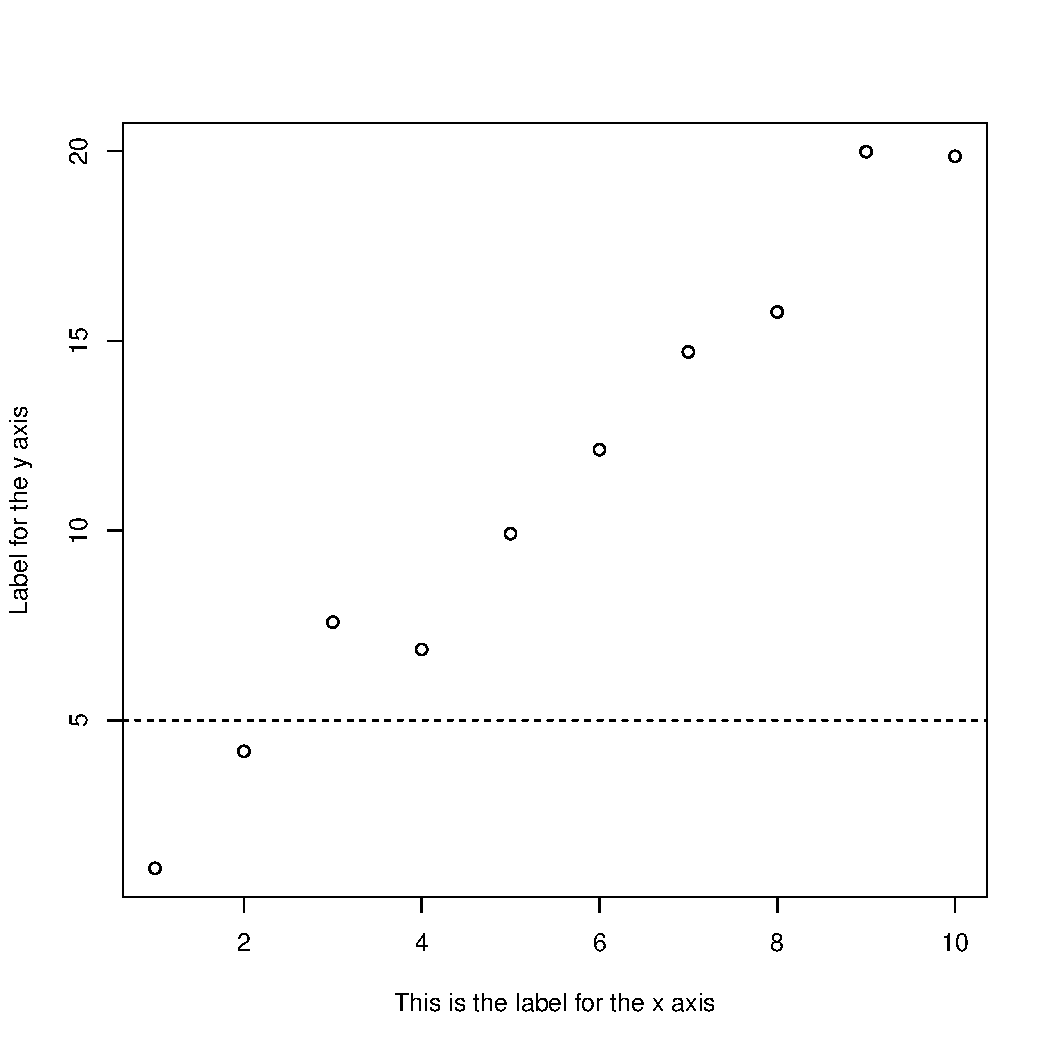
\includegraphics[width=\maxwidth]{figure/unnamed-chunk-72-1} 
\end{knitrout}

\section{Personalización de plots: colores, tipos de línea y de puntos}
Se pueden personalizar los gráficos añadiendo colores específicos, modificando el tipo de línea y de puntos.
\begin{knitrout}
\definecolor{shadecolor}{rgb}{0.969, 0.969, 0.969}\color{fgcolor}\begin{kframe}
\begin{alltt}
\hlkwd{plot}\hldef{(}\hlkwd{c}\hldef{(}\hlnum{1}\hldef{,} \hlnum{21}\hldef{),} \hlkwd{c}\hldef{(}\hlnum{1}\hldef{,} \hlnum{2.3}\hldef{),}
     \hlkwc{type} \hldef{=} \hlsng{"n"}\hldef{,} \hlkwc{axes} \hldef{=} \hlnum{FALSE}\hldef{,} \hlkwc{ann} \hldef{=} \hlnum{FALSE}\hldef{)}
\hlcom{## show pch}
\hlkwd{points}\hldef{(}\hlnum{1}\hlopt{:}\hlnum{20}\hldef{,} \hlkwd{rep}\hldef{(}\hlnum{1}\hldef{,} \hlnum{20}\hldef{),} \hlkwc{pch} \hldef{=} \hlnum{1}\hlopt{:}\hlnum{20}\hldef{)}
\hlkwd{text}\hldef{(}\hlnum{1}\hlopt{:}\hlnum{20}\hldef{,} \hlnum{1.2}\hldef{,} \hlkwc{labels} \hldef{=} \hlnum{1}\hlopt{:}\hlnum{20}\hldef{)}
\hlkwd{text}\hldef{(}\hlnum{11}\hldef{,} \hlnum{1.5}\hldef{,} \hlsng{"pch"}\hldef{,} \hlkwc{cex} \hldef{=} \hlnum{1.3}\hldef{)}

\hlcom{## show colors for rainbow palette}
\hlkwd{points}\hldef{(}\hlnum{1}\hlopt{:}\hlnum{20}\hldef{,} \hlkwd{rep}\hldef{(}\hlnum{2}\hldef{,} \hlnum{20}\hldef{),} \hlkwc{pch} \hldef{=} \hlnum{16}\hldef{,} \hlkwc{col} \hldef{=} \hlkwd{rainbow}\hldef{(}\hlnum{20}\hldef{))}
\hlkwd{text}\hldef{(}\hlnum{11}\hldef{,} \hlnum{2.2}\hldef{,} \hlsng{"col"}\hldef{,} \hlkwc{cex} \hldef{=} \hlnum{1.3}\hldef{)}
\end{alltt}
\end{kframe}\begin{figure}
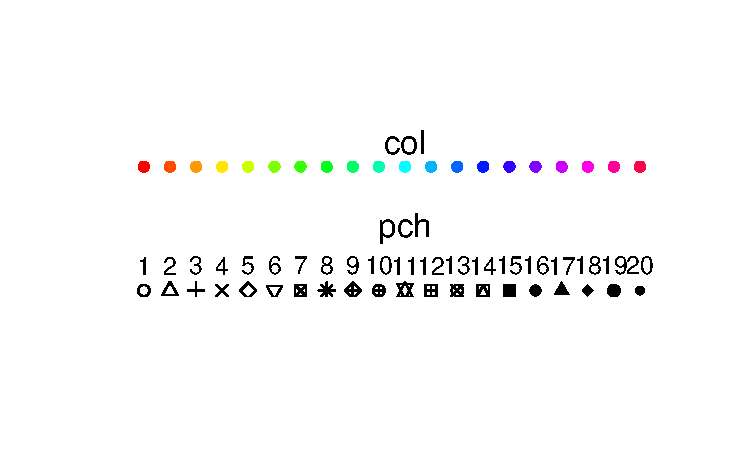
\includegraphics[width=\maxwidth]{figure/pchcol-1} \caption[pch and col]{pch and col}\label{fig:pchcol}
\end{figure}

\end{knitrout}

\begin{knitrout}
\definecolor{shadecolor}{rgb}{0.969, 0.969, 0.969}\color{fgcolor}\begin{kframe}
\begin{alltt}
\hlkwd{plot}\hldef{(}\hlkwd{c}\hldef{(}\hlnum{0.2}\hldef{,} \hlnum{5}\hldef{),} \hlkwd{c}\hldef{(}\hlnum{0.2}\hldef{,} \hlnum{5}\hldef{),} \hlkwc{type} \hldef{=} \hlsng{"n"}\hldef{,} \hlkwc{ann} \hldef{=} \hlnum{FALSE}\hldef{,} \hlkwc{axes} \hldef{=} \hlnum{FALSE}\hldef{)}
\hlkwa{for}\hldef{(i} \hlkwa{in} \hlnum{1}\hlopt{:}\hlnum{6}\hldef{) \{}
    \hlkwd{abline}\hldef{(}\hlnum{0}\hldef{, i}\hlopt{/}\hlnum{3}\hldef{,} \hlkwc{lty} \hldef{= i,} \hlkwc{lwd} \hldef{=} \hlnum{2}\hldef{)}
    \hlkwd{text}\hldef{(}\hlnum{2}\hldef{,} \hlnum{2} \hlopt{*} \hldef{(i}\hlopt{/}\hlnum{3}\hldef{),} \hlkwc{labels} \hldef{= i,} \hlkwc{pos} \hldef{=} \hlnum{3}\hldef{)}
\hldef{\}}
\end{alltt}
\end{kframe}\begin{figure}
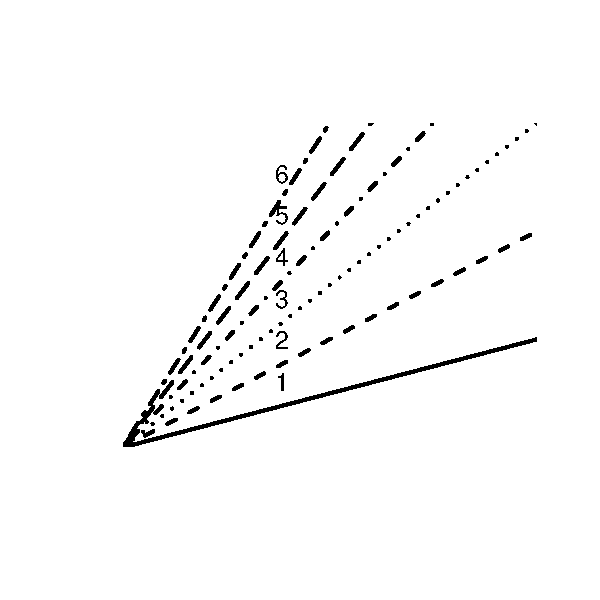
\includegraphics[width=\maxwidth]{figure/ltytype-1} \caption[lty for values 1 to 6]{lty for values 1 to 6}\label{fig:ltytype}
\end{figure}

\end{knitrout}

\subsection{Un ejemplo de cómo mejorar gráficos}
El gráfico básico sería el siguiente:
\begin{knitrout}
\definecolor{shadecolor}{rgb}{0.969, 0.969, 0.969}\color{fgcolor}\begin{kframe}
\begin{alltt}
\hldef{hit} \hlkwb{<-} \hlkwd{read.table}\hldef{(}\hlsng{"data/hit-table-500-text.txt"}\hldef{)}
\hlcom{## We know, from the header of the file, that}
\hlcom{## alignment length is the fifth column,}
\hlcom{## score is the 13th and percent identity the 3rd}
\hlkwd{hist}\hldef{(hit[,} \hlnum{5}\hldef{])} \hlcom{## the histogram}
\end{alltt}
\end{kframe}
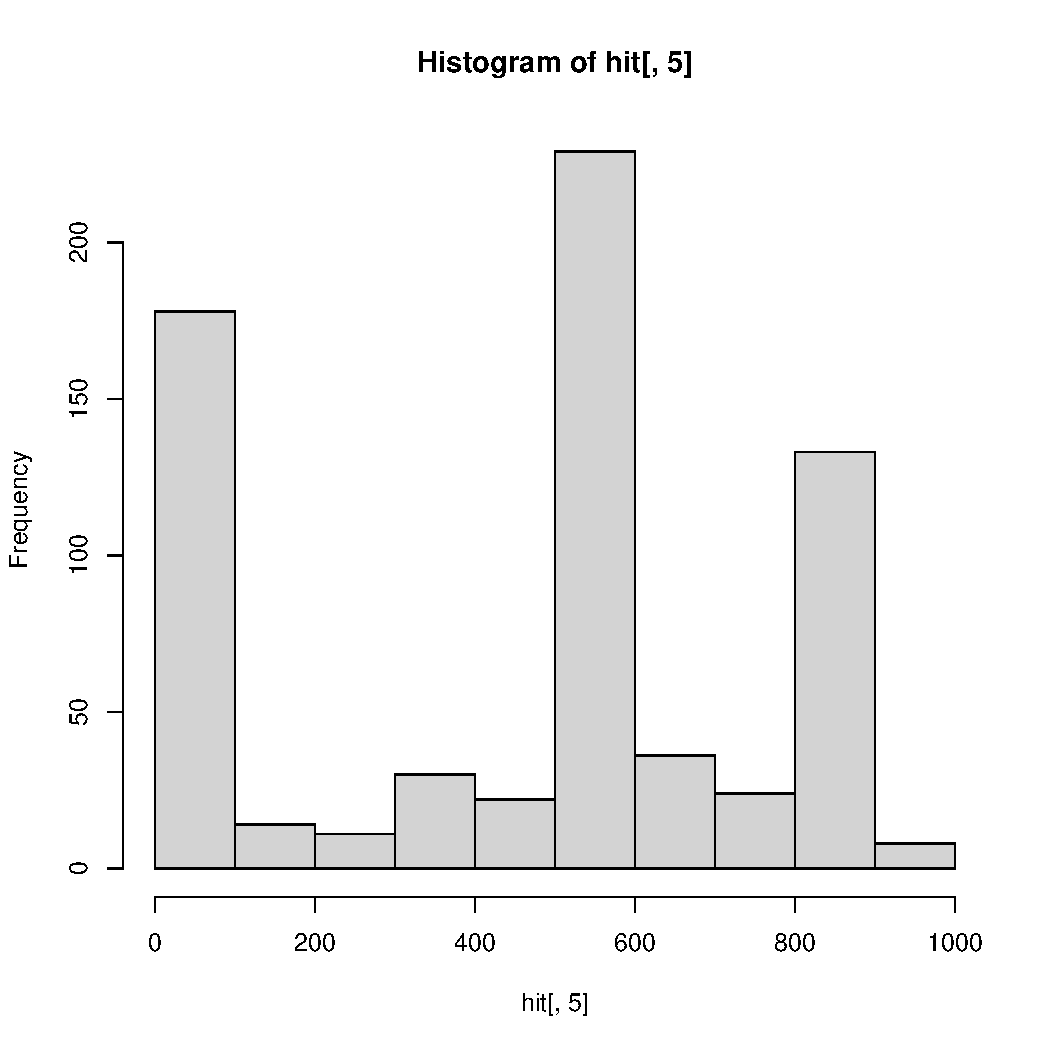
\includegraphics[width=\maxwidth]{figure/unnamed-chunk-73-1} 
\begin{kframe}\begin{alltt}
\hlkwd{plot}\hldef{(hit[,} \hlnum{13}\hldef{]} \hlopt{~} \hldef{hit[,} \hlnum{3}\hldef{])} \hlcom{## the scatterplot}
\end{alltt}
\end{kframe}
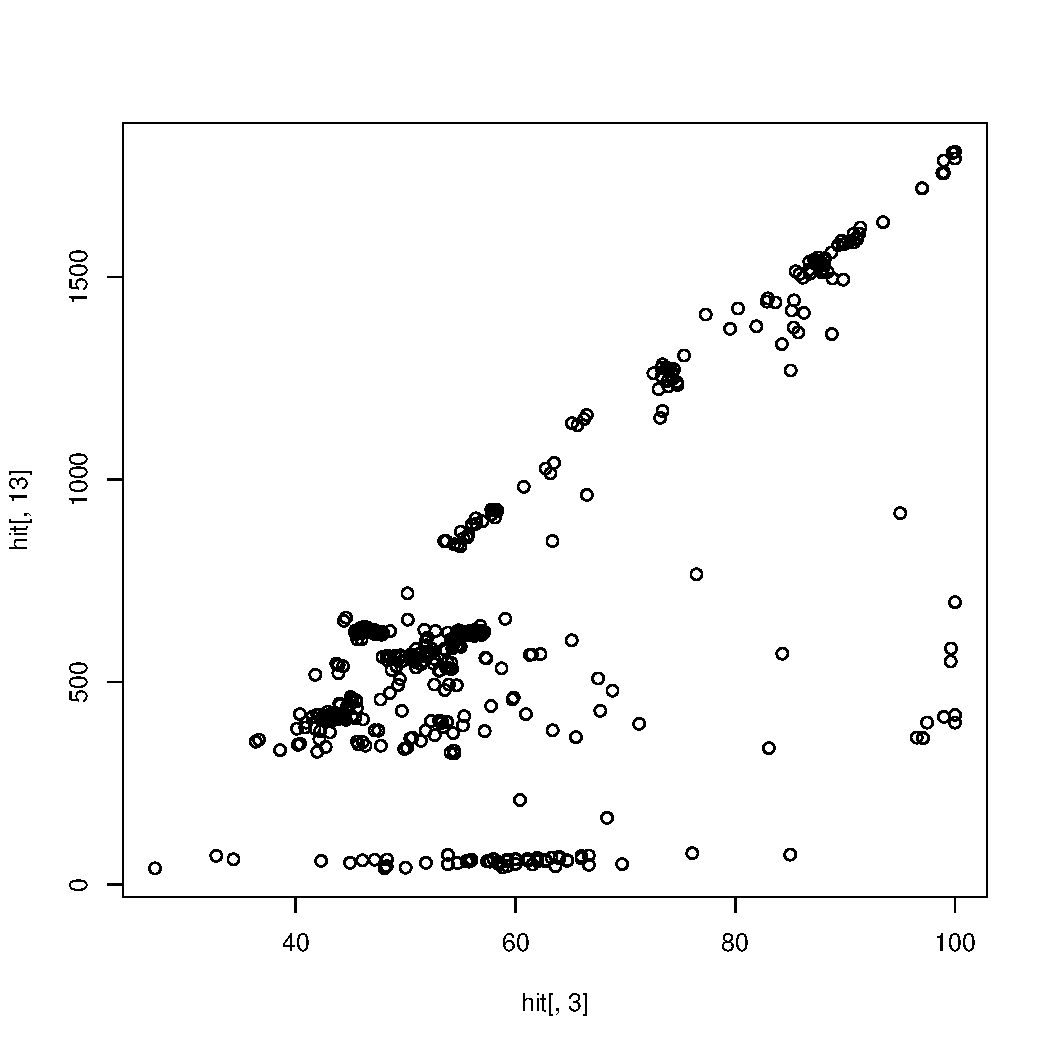
\includegraphics[width=\maxwidth]{figure/unnamed-chunk-73-2} 
\begin{kframe}\begin{alltt}
\hlcom{## plot(y ~ x) == plot(x, y)}
\end{alltt}
\end{kframe}
\end{knitrout}

Pero esto es fácilmente mejorable:
\begin{knitrout}
\definecolor{shadecolor}{rgb}{0.969, 0.969, 0.969}\color{fgcolor}\begin{kframe}
\begin{alltt}
\hlkwd{par}\hldef{(}\hlkwc{mfrow} \hldef{=} \hlkwd{c}\hldef{(}\hlnum{1}\hldef{,} \hlnum{2}\hldef{))} \hlcom{## two figures side by side}
\hlkwd{hist}\hldef{(hit[,} \hlnum{5}\hldef{],} \hlkwc{breaks} \hldef{=} \hlnum{50}\hldef{,} \hlkwc{xlab} \hldef{=} \hlsng{""}\hldef{,} \hlkwc{main} \hldef{=} \hlsng{"Alignment length"}\hldef{)}
\hlkwd{plot}\hldef{(hit[,} \hlnum{13}\hldef{]} \hlopt{~} \hldef{hit[,} \hlnum{3}\hldef{],} \hlkwc{xlab} \hldef{=} \hlsng{"Percent. identity"}\hldef{,}
     \hlkwc{ylab} \hldef{=} \hlsng{"Bit score"}\hldef{)}
\end{alltt}
\end{kframe}\begin{figure}
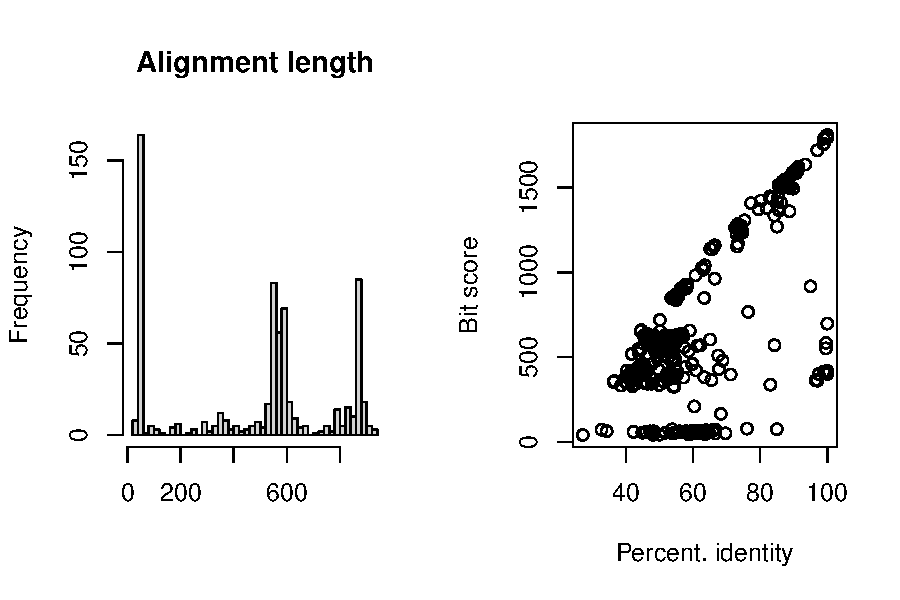
\includegraphics[width=\maxwidth]{figure/fig-blast-1} \caption[A quick look at the alignment results]{A quick look at the alignment results}\label{fig-blast}
\end{figure}

\end{knitrout}

Por simetría, se podría añadir un título al segundo gráfico. También se pueden generar gráficos interactivos con la librería \code{car}.
\begin{knitrout}
\definecolor{shadecolor}{rgb}{0.969, 0.969, 0.969}\color{fgcolor}\begin{kframe}
\begin{alltt}
\hlkwd{library}\hldef{(car)}
\hlkwd{scatter3d}\hldef{(hit[,} \hlnum{13}\hldef{]} \hlopt{~} \hldef{hit[,} \hlnum{3}\hldef{]} \hlopt{+} \hldef{hit[,} \hlnum{5}\hldef{],} \hlkwc{xlab} \hldef{=} \hlsng{"Ident"}\hldef{,}
          \hlkwc{zlab} \hldef{=} \hlsng{"Length"}\hldef{,} \hlkwc{ylab} \hldef{=} \hlsng{"Score"}\hldef{)}
\end{alltt}
\end{kframe}
\end{knitrout}

\section{Guardar plots}
Se pueden guardar las gráficas como PDF, png, etc. Desde RStudio hay una ventana de gráficos. Sin embargo, es mejor especificar y determinar unas características como tamaño, extensión, etc. Se pueden utilizar las funciones \code{pdf()} y \code{png()}: \code{pdf(file="plot.pdf")}. El paquete ggplot tiene la función \code{ggsave()}.

En el siguiente ejemplo se abre un PDF, se generan dos gráficos y hasta que no se ejecuta \code{dev.off()} no se guarda el contenido en el PDF. Además, cada gráfico se guarda en una página distinta del PDF. 
\begin{knitrout}
\definecolor{shadecolor}{rgb}{0.969, 0.969, 0.969}\color{fgcolor}\begin{kframe}
\begin{alltt}
\hlkwd{pdf}\hldef{(}\hlkwc{file} \hldef{=} \hlsng{"file1.pdf"}\hldef{,} \hlkwc{width} \hldef{=} \hlnum{2}\hldef{,} \hlkwc{heigh} \hldef{=} \hlnum{3}\hldef{)}
\hlkwd{plot}\hldef{(}\hlnum{1}\hlopt{:}\hlnum{10}\hldef{)}
\hlkwd{abline}\hldef{(}\hlkwc{h} \hldef{=} \hlnum{4}\hldef{,} \hlkwc{lty} \hldef{=} \hlnum{2}\hldef{,} \hlkwc{col} \hldef{=} \hlsng{"blue"}\hldef{)}
\hlkwd{hist}\hldef{(}\hlkwd{rnorm}\hldef{(}\hlnum{25}\hldef{))}
\hlkwd{dev.off}\hldef{()}
\end{alltt}
\end{kframe}
\end{knitrout}

\section{Tipos de gráficos}
Hemos visto que \code{plot} genera un gráfico simple de puntos, pero hay más tipos. Por ejemplo, \code{hist} genera un histograma. En el paquete de \code{ggplot2} hay más opciones de tipos de gráficos con una mayor posibilidad de personalización.

El paquete \code{car} también cuenta con varios tipos de gráficos, como scatter3d mencionado anteriormente. También tiene una función llamada \code{scatterplot}:

\begin{knitrout}
\definecolor{shadecolor}{rgb}{0.969, 0.969, 0.969}\color{fgcolor}\begin{kframe}
\begin{alltt}
\hlkwd{library}\hldef{(car)}
\end{alltt}


{\ttfamily\noindent\itshape\color{messagecolor}{\#\# Cargando paquete requerido: carData}}\begin{alltt}
\hlkwd{load}\hldef{(}\hlsng{"data/anage.RData"}\hldef{)}
\hlkwd{scatterplot}\hldef{(Metabolic.rate..W.} \hlopt{~} \hldef{Body.mass..g.,} \hlkwc{log}\hldef{=}\hlsng{"xy"}\hldef{,}
            \hlkwc{data} \hldef{= anage)}
\end{alltt}
\end{kframe}
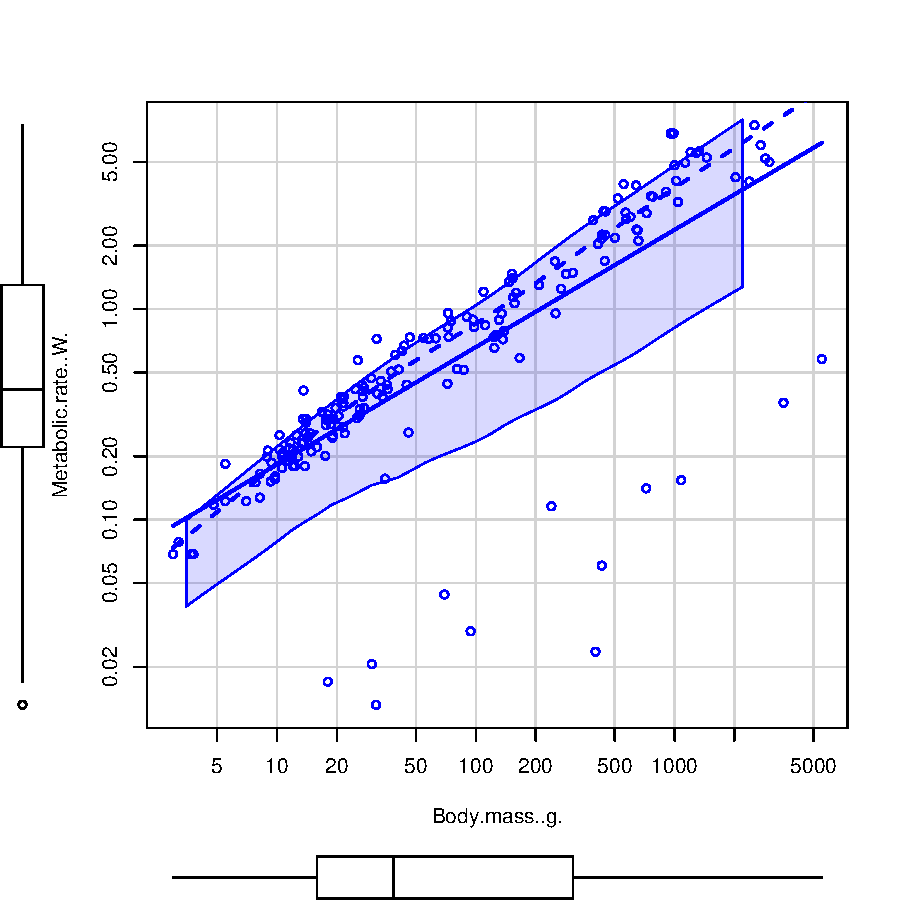
\includegraphics[width=\maxwidth]{figure/mrateplotx1-1} 
\end{knitrout}

Dependiendo de la figura final que se quiera, se puede ir añadiendo elementos desde plot o utilizar scatterplot y eliminar cosas.

Las leyendas se introducen con la función \code{legend} en caso de utilizar plot.

\begin{knitrout}
\definecolor{shadecolor}{rgb}{0.969, 0.969, 0.969}\color{fgcolor}\begin{kframe}
\begin{alltt}
\hlkwd{plot}\hldef{(Metabolic.rate..W.} \hlopt{~} \hldef{Body.mass..g.,} \hlkwc{log}\hldef{=}\hlsng{"xy"}\hldef{,}
     \hlkwc{col} \hldef{=} \hlkwd{c}\hldef{(}\hlsng{"salmon"}\hldef{,} \hlsng{"darkgreen"}\hldef{)[Class],} \hlkwc{data} \hldef{= anage)}
\hlkwd{legend}\hldef{(}\hlnum{5}\hldef{,} \hlnum{5}\hldef{,} \hlkwc{legend} \hldef{=} \hlkwd{levels}\hldef{(anage}\hlopt{$}\hldef{Class),}
       \hlkwc{col} \hldef{=} \hlkwd{c}\hldef{(}\hlsng{"salmon"}\hldef{,} \hlsng{"darkgreen"}\hldef{),}
       \hlkwc{pch} \hldef{=} \hlnum{1}\hldef{)}
\end{alltt}
\end{kframe}
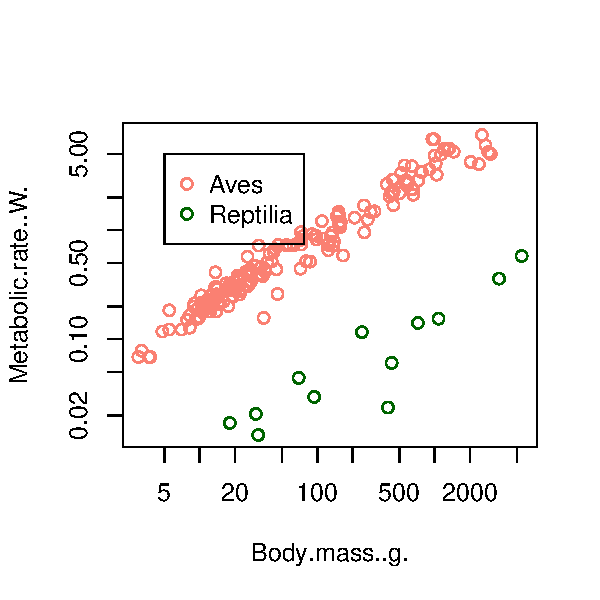
\includegraphics[width=\maxwidth]{figure/unnamed-chunk-76-1} 
\end{knitrout}

Si se utiliza scatterplot, la sintaxis es diferente y añade directamente la línea de regresión:
\begin{knitrout}
\definecolor{shadecolor}{rgb}{0.969, 0.969, 0.969}\color{fgcolor}\begin{kframe}
\begin{alltt}
\hlkwd{scatterplot}\hldef{(Metabolic.rate..W.} \hlopt{~} \hldef{Body.mass..g.}\hlopt{|}\hldef{Class,} \hlkwc{log}\hldef{=}\hlsng{"xy"}\hldef{,}
            \hlkwc{data} \hldef{= anage)}
\end{alltt}
\end{kframe}
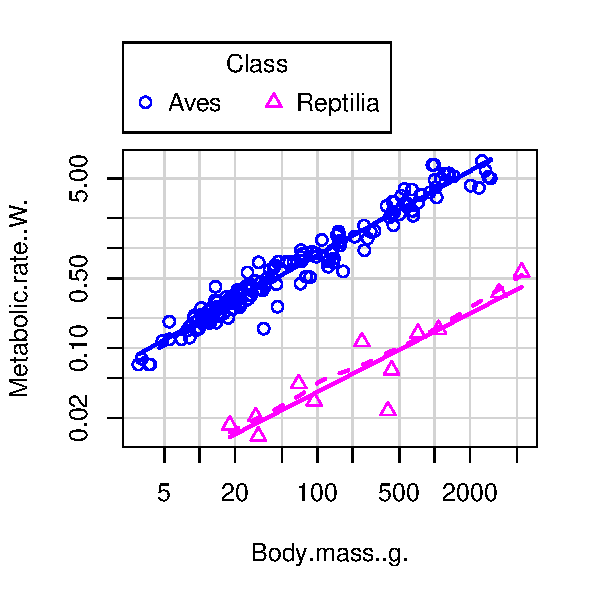
\includegraphics[width=\maxwidth]{figure/unnamed-chunk-77-1} 
\end{knitrout}

\chapter{Tablas}
Tabular datos es una operación muy común. Hay fundamentalmente dos formas de realizarlo con \code{table} (la más sencilla) y \code{xtabs} (con uso más genérico):
\begin{knitrout}
\definecolor{shadecolor}{rgb}{0.969, 0.969, 0.969}\color{fgcolor}\begin{kframe}
\begin{alltt}
\hlkwd{table}\hldef{(AB2}\hlopt{$}\hldef{Sex, AB2}\hlopt{$}\hldef{status)}
\end{alltt}
\begin{verbatim}
##    
##     V Z
##   F 1 2
##   M 2 1
\end{verbatim}
\begin{alltt}
\hlkwd{with}\hldef{(AB2,} \hlkwd{table}\hldef{(Sex, status))} \hlcom{## note "with"}
\end{alltt}
\begin{verbatim}
##    status
## Sex V Z
##   F 1 2
##   M 2 1
\end{verbatim}
\begin{alltt}
\hlkwd{xtabs}\hldef{(} \hlopt{~} \hldef{Sex} \hlopt{+} \hldef{status,} \hlkwc{data} \hldef{= AB2)}
\end{alltt}
\begin{verbatim}
##    status
## Sex V Z
##   F 1 2
##   M 2 1
\end{verbatim}
\end{kframe}
\end{knitrout}

Tabular un dataframe completo saca varias tablas 2x2 en función de las combinaciones de los valores de las otras variables. 

\section{Más de dos dimensiones y \code{ftable}}
Cuando hay más de dos dimensiones, utilizar las funciones anteriores saca el mismo resultado. 
\begin{knitrout}
\definecolor{shadecolor}{rgb}{0.969, 0.969, 0.969}\color{fgcolor}\begin{kframe}
\begin{alltt}
\hldef{(x} \hlkwb{<-}  \hlkwd{data.frame}\hldef{(}\hlkwc{a} \hldef{=} \hlkwd{c}\hldef{(}\hlnum{1}\hldef{,}\hlnum{2}\hldef{,}\hlnum{2}\hldef{,}\hlnum{1}\hldef{,}\hlnum{2}\hldef{,}\hlnum{2}\hldef{,}\hlnum{1}\hldef{),}
                 \hlkwc{b} \hldef{=} \hlkwd{c}\hldef{(}\hlnum{1}\hldef{,}\hlnum{2}\hldef{,}\hlnum{2}\hldef{,}\hlnum{1}\hldef{,}\hlnum{1}\hldef{,}\hlnum{2}\hldef{,}\hlnum{1}\hldef{),}
                 \hlkwc{c} \hldef{=} \hlkwd{c}\hldef{(}\hlnum{1}\hldef{,}\hlnum{1}\hldef{,}\hlnum{2}\hldef{,}\hlnum{1}\hldef{,}\hlnum{2}\hldef{,}\hlnum{2}\hldef{,}\hlnum{1}\hldef{)))}
\end{alltt}
\begin{verbatim}
##   a b c
## 1 1 1 1
## 2 2 2 1
## 3 2 2 2
## 4 1 1 1
## 5 2 1 2
## 6 2 2 2
## 7 1 1 1
\end{verbatim}
\begin{alltt}
\hlcom{## Equivalent}
\hlkwd{table}\hldef{(x)}
\end{alltt}
\begin{verbatim}
## , , c = 1
## 
##    b
## a   1 2
##   1 3 0
##   2 0 1
## 
## , , c = 2
## 
##    b
## a   1 2
##   1 0 0
##   2 1 2
\end{verbatim}
\begin{alltt}
\hlkwd{xtabs}\hldef{(}\hlopt{~} \hldef{a} \hlopt{+} \hldef{b} \hlopt{+} \hldef{c,} \hlkwc{data} \hldef{= x)}
\end{alltt}
\begin{verbatim}
## , , c = 1
## 
##    b
## a   1 2
##   1 3 0
##   2 0 1
## 
## , , c = 2
## 
##    b
## a   1 2
##   1 0 0
##   2 1 2
\end{verbatim}
\end{kframe}
\end{knitrout}

Sin embargo, hay veces en las que buscamos una tabla plana, es decir, encajar una de las variables dentro de otra:
\begin{knitrout}
\definecolor{shadecolor}{rgb}{0.969, 0.969, 0.969}\color{fgcolor}\begin{kframe}
\begin{alltt}
\hlkwd{ftable}\hldef{(}\hlkwd{xtabs}\hldef{(}\hlopt{~} \hldef{a} \hlopt{+} \hldef{b} \hlopt{+} \hldef{c,} \hlkwc{data} \hldef{= x))}
\end{alltt}
\begin{verbatim}
##     c 1 2
## a b      
## 1 1   3 0
##   2   0 0
## 2 1   0 1
##   2   1 2
\end{verbatim}
\begin{alltt}
\hlcom{## same as ftable(table(x))}
\end{alltt}
\end{kframe}
\end{knitrout}

\section{Recuperar una tabla de un dataframe}
Si una tabla se nos ha convertido en un dataframe, se puede volver a convertir en tabla:

\begin{knitrout}
\definecolor{shadecolor}{rgb}{0.969, 0.969, 0.969}\color{fgcolor}\begin{kframe}
\begin{alltt}
\hlcom{## create a data frame with a "Freq" column:}
\hlcom{## put the table in a data frame}
\hldef{(dfx} \hlkwb{<-} \hlkwd{as.data.frame}\hldef{(}\hlkwd{table}\hldef{(x)))}
\end{alltt}
\begin{verbatim}
##   a b c Freq
## 1 1 1 1    3
## 2 2 1 1    0
## 3 1 2 1    0
## 4 2 2 1    1
## 5 1 1 2    0
## 6 2 1 2    1
## 7 1 2 2    0
## 8 2 2 2    2
\end{verbatim}
\begin{alltt}
\hlcom{## We can recover the table}
\hlkwd{xtabs}\hldef{(Freq} \hlopt{~} \hldef{a} \hlopt{+} \hldef{b} \hlopt{+} \hldef{c,} \hlkwc{data} \hldef{= dfx)}
\end{alltt}
\begin{verbatim}
## , , c = 1
## 
##    b
## a   1 2
##   1 3 0
##   2 0 1
## 
## , , c = 2
## 
##    b
## a   1 2
##   1 0 0
##   2 1 2
\end{verbatim}
\begin{alltt}
\hlcom{## of course, this is the same as}
\hlcom{## xtabs(~ a + b + c, data = x)}
\hlcom{## or table(x)}
\end{alltt}
\end{kframe}
\end{knitrout}

%25/10 - Ramón
\chapter{La familia \code{apply}}
Una de las grandes ventajas de R es poder operar sobre vectores, arrays, listas, etc enteros. Algunas funciones son \code{apply, lapply, sapply, tapply, mapply}. 

\section{apply}
apply es una forma de utilizar una función sobre una cierta cantidad de elementos. Es una forma más elegante que realizando un bucle. 

\begin{knitrout}
\definecolor{shadecolor}{rgb}{0.969, 0.969, 0.969}\color{fgcolor}\begin{kframe}
\begin{alltt}
\hldef{(Z} \hlkwb{<-} \hlkwd{matrix}\hldef{(}\hlkwd{c}\hldef{(}\hlnum{1}\hldef{,} \hlnum{27}\hldef{,} \hlnum{23}\hldef{,} \hlnum{13}\hldef{),} \hlkwc{nrow} \hldef{=} \hlnum{2}\hldef{))}
\end{alltt}
\begin{verbatim}
##      [,1] [,2]
## [1,]    1   23
## [2,]   27   13
\end{verbatim}
\begin{alltt}
\hlkwd{apply}\hldef{(Z,} \hlnum{1}\hldef{, median)}
\end{alltt}
\begin{verbatim}
## [1] 12 20
\end{verbatim}
\begin{alltt}
\hlkwd{apply}\hldef{(Z,} \hlnum{2}\hldef{, median)}
\end{alltt}
\begin{verbatim}
## [1] 14 18
\end{verbatim}
\begin{alltt}
\hlkwd{apply}\hldef{(Z,} \hlnum{2}\hldef{, min)}
\end{alltt}
\begin{verbatim}
## [1]  1 13
\end{verbatim}
\end{kframe}
\end{knitrout}

\section{lapply}
Con listas se utiliza \code{lapply}, y aplica una función definida a esa lista. 

\begin{knitrout}
\definecolor{shadecolor}{rgb}{0.969, 0.969, 0.969}\color{fgcolor}\begin{kframe}
\begin{alltt}
\hldef{(listA} \hlkwb{<-} \hlkwd{list}\hldef{(}\hlkwc{one.vector} \hldef{=} \hlnum{1}\hlopt{:}\hlnum{10}\hldef{,}  \hlkwc{hello} \hldef{=} \hlsng{"Hola"}\hldef{,}
               \hlkwc{one.matrix} \hldef{=} \hlkwd{matrix}\hldef{(}\hlkwd{rnorm}\hldef{(}\hlnum{20}\hldef{),} \hlkwc{ncol} \hldef{=} \hlnum{5}\hldef{),}
               \hlkwc{another.list} \hldef{=} \hlkwd{list}\hldef{(}\hlkwc{a} \hldef{=} \hlnum{5}\hldef{,}
                 \hlkwc{b} \hldef{=} \hlkwd{factor}\hldef{(}\hlkwd{c}\hldef{(}\hlsng{"male"}\hldef{,} \hlsng{"female"}\hldef{,} \hlsng{"female"}\hldef{)))))}
\end{alltt}
\begin{verbatim}
## $one.vector
##  [1]  1  2  3  4  5  6  7  8  9 10
## 
## $hello
## [1] "Hola"
## 
## $one.matrix
##            [,1]        [,2]       [,3]         [,4]       [,5]
## [1,]  0.4176508  1.78222896  1.0128287  1.589638200  0.4772373
## [2,]  0.9817528 -2.31106908  0.4322652  1.954651642 -0.5965582
## [3,] -0.3926954  0.87860458  2.0908192  0.004937777  0.7922033
## [4,] -1.0396690  0.03580672 -1.1999258 -2.451706388  0.2896367
## 
## $another.list
## $another.list$a
## [1] 5
## 
## $another.list$b
## [1] male   female female
## Levels: female male
\end{verbatim}
\begin{alltt}
\hlkwd{lapply}\hldef{(listA,} \hlkwa{function}\hldef{(}\hlkwc{x}\hldef{) x[[}\hlnum{1}\hldef{]])}
\end{alltt}
\begin{verbatim}
## $one.vector
## [1] 1
## 
## $hello
## [1] "Hola"
## 
## $one.matrix
## [1] 0.4176508
## 
## $another.list
## [1] 5
\end{verbatim}
\end{kframe}
\end{knitrout}

\section{tapply y by}
Se utiliza \code{tapply} cuando tenemos unos datos (una columna o varias) que se pueden utilizar para estratificar o seleccionar otros datos. Los dos vectores u objetos deben tener la misma longitud. 

\begin{knitrout}
\definecolor{shadecolor}{rgb}{0.969, 0.969, 0.969}\color{fgcolor}\begin{kframe}
\begin{alltt}
\hldef{(one.dataframe} \hlkwb{<-} \hlkwd{data.frame}\hldef{(}\hlkwc{age} \hldef{=} \hlkwd{c}\hldef{(}\hlnum{12}\hldef{,} \hlnum{13}\hldef{,} \hlnum{16}\hldef{,} \hlnum{25}\hldef{,} \hlnum{28}\hldef{),}
                            \hlkwc{sex} \hldef{=} \hlkwd{factor}\hldef{(}\hlkwd{c}\hldef{(}\hlsng{"male"}\hldef{,} \hlsng{"female"}\hldef{,}
                                           \hlsng{"female"}\hldef{,} \hlsng{"male"}\hldef{,} \hlsng{"male"}\hldef{)))}
\hldef{)}
\end{alltt}
\begin{verbatim}
##   age    sex
## 1  12   male
## 2  13 female
## 3  16 female
## 4  25   male
## 5  28   male
\end{verbatim}
\begin{alltt}
\hldef{one.dataframe} \hlkwb{<-} \hlkwd{rbind}\hldef{(one.dataframe, one.dataframe)}
\hldef{one.dataframe}\hlopt{$}\hldef{age[}\hlnum{6}\hlopt{:}\hlnum{10}\hldef{]} \hlkwb{<-} \hldef{one.dataframe}\hlopt{$}\hldef{age[}\hlnum{6}\hlopt{:}\hlnum{10}\hldef{]} \hlopt{+} \hlnum{2}
\hldef{one.dataframe}\hlopt{$}\hldef{country} \hlkwb{<-} \hlkwd{rep}\hldef{(}\hlkwd{c}\hldef{(}\hlsng{"A"}\hldef{,} \hlsng{"B"}\hldef{),} \hlkwd{c}\hldef{(}\hlnum{5}\hldef{,} \hlnum{5}\hldef{))}
\hldef{one.dataframe}\hlopt{$}\hldef{Y} \hlkwb{<-} \hlkwd{rnorm}\hldef{(}\hlnum{10}\hldef{)}
\hldef{one.dataframe}
\end{alltt}
\begin{verbatim}
##    age    sex country          Y
## 1   12   male       A  0.7389386
## 2   13 female       A  0.3189604
## 3   16 female       A  1.0761644
## 4   25   male       A -0.2841577
## 5   28   male       A -0.7766753
## 6   14   male       B -0.5956605
## 7   15 female       B -1.7259798
## 8   18 female       B -0.9025845
## 9   27   male       B -0.5590619
## 10  30   male       B -0.2465126
\end{verbatim}
\begin{alltt}
\hlkwd{tapply}\hldef{(one.dataframe}\hlopt{$}\hldef{age, one.dataframe}\hlopt{$}\hldef{sex, mean)}
\end{alltt}
\begin{verbatim}
##   female     male 
## 15.50000 22.66667
\end{verbatim}
\end{kframe}
\end{knitrout}

Se pueden formar grupos con dos o más variables siempre y cuando se proporcionen en forma de lista:
\begin{knitrout}
\definecolor{shadecolor}{rgb}{0.969, 0.969, 0.969}\color{fgcolor}\begin{kframe}
\begin{alltt}
\hlkwd{tapply}\hldef{(one.dataframe}\hlopt{$}\hldef{age,}
       \hlkwd{list}\hldef{(one.dataframe}\hlopt{$}\hldef{sex, one.dataframe}\hlopt{$}\hldef{country),}
       \hldef{mean)}
\end{alltt}
\begin{verbatim}
##               A        B
## female 14.50000 16.50000
## male   21.66667 23.66667
\end{verbatim}
\end{kframe}
\end{knitrout}

De igual forma, se puede utilizar una función que devuelva más que un solo valor:
\begin{knitrout}
\definecolor{shadecolor}{rgb}{0.969, 0.969, 0.969}\color{fgcolor}\begin{kframe}
\begin{alltt}
\hlkwd{tapply}\hldef{(one.dataframe}\hlopt{$}\hldef{age,}
       \hldef{one.dataframe}\hlopt{$}\hldef{sex,}
       \hlkwa{function}\hldef{(}\hlkwc{x}\hldef{)} \hlkwd{c}\hldef{(}\hlkwc{Mean} \hldef{=} \hlkwd{mean}\hldef{(x),} \hlkwc{Var} \hldef{=} \hlkwd{var}\hldef{(x)))}
\end{alltt}
\begin{verbatim}
## $female
##      Mean       Var 
## 15.500000  4.333333 
## 
## $male
##     Mean      Var 
## 22.66667 59.06667
\end{verbatim}
\end{kframe}
\end{knitrout}
El problema con esto viene cuando se quiere realizar lo anterior en base a dos o más variables. Para estos casos, se debería emplear \code{aggregate}.

La función \code{by} es similar a tapply, pero para dataframes. Las salidas de ambas funciones también son diferentes:
\begin{knitrout}
\definecolor{shadecolor}{rgb}{0.969, 0.969, 0.969}\color{fgcolor}\begin{kframe}
\begin{alltt}
\hlkwd{by}\hldef{(one.dataframe,}
   \hlkwd{list}\hldef{(one.dataframe}\hlopt{$}\hldef{sex, one.dataframe}\hlopt{$}\hldef{country),}
   \hlkwa{function}\hldef{(}\hlkwc{x}\hldef{)} \hlkwd{c}\hldef{(}\hlkwc{Mean_Age} \hldef{=} \hlkwd{mean}\hldef{(x}\hlopt{$}\hldef{age),} \hlkwc{SD_Age} \hldef{=} \hlkwd{sd}\hldef{(x}\hlopt{$}\hldef{age),}
                 \hlkwc{Median_Y} \hldef{=} \hlkwd{median}\hldef{(x}\hlopt{$}\hldef{Y)))}
\end{alltt}
\begin{verbatim}
## : female
## : A
##   Mean_Age     SD_Age   Median_Y 
## 14.5000000  2.1213203  0.6975624 
## ------------------------------------------------ 
## : male
## : A
##   Mean_Age     SD_Age   Median_Y 
## 21.6666667  8.5049005 -0.2841577 
## ------------------------------------------------ 
## : female
## : B
##  Mean_Age    SD_Age  Median_Y 
## 16.500000  2.121320 -1.314282 
## ------------------------------------------------ 
## : male
## : B
##   Mean_Age     SD_Age   Median_Y 
## 23.6666667  8.5049005 -0.5590619
\end{verbatim}
\end{kframe}
\end{knitrout}

\section{aggregate}
La función \code{aggregate} suele devolver la salida en un formato más conveniente. En este caso, el segundo argumento debe ser siempre una lista:
\begin{knitrout}
\definecolor{shadecolor}{rgb}{0.969, 0.969, 0.969}\color{fgcolor}\begin{kframe}
\begin{alltt}
\hlkwd{aggregate}\hldef{(one.dataframe}\hlopt{$}\hldef{age,} \hlkwd{list}\hldef{(one.dataframe}\hlopt{$}\hldef{sex), mean)}
\end{alltt}
\begin{verbatim}
##   Group.1        x
## 1  female 15.50000
## 2    male 22.66667
\end{verbatim}
\begin{alltt}
\hlcom{## make the aggregating variable explicit,}
\hlcom{## and give it another name}
\hlkwd{aggregate}\hldef{(one.dataframe}\hlopt{$}\hldef{age,}
          \hlkwd{list}\hldef{(}\hlkwc{Sexo} \hldef{= one.dataframe}\hlopt{$}\hldef{sex), mean)}
\end{alltt}
\begin{verbatim}
##     Sexo        x
## 1 female 15.50000
## 2   male 22.66667
\end{verbatim}
\begin{alltt}
\hlcom{## or use the name of the column/variable}
\hlkwd{aggregate}\hldef{(one.dataframe}\hlopt{$}\hldef{age,}
          \hldef{one.dataframe[}\hlnum{2}\hldef{], mean)}
\end{alltt}
\begin{verbatim}
##      sex        x
## 1 female 15.50000
## 2   male 22.66667
\end{verbatim}
\end{kframe}
\end{knitrout}

Se puede utilizar con dos o más variables:
\begin{knitrout}
\definecolor{shadecolor}{rgb}{0.969, 0.969, 0.969}\color{fgcolor}\begin{kframe}
\begin{alltt}
\hlkwd{aggregate}\hldef{(one.dataframe}\hlopt{$}\hldef{age,}
          \hlkwd{list}\hldef{(}\hlkwc{Sex} \hldef{= one.dataframe}\hlopt{$}\hldef{sex,}
               \hlkwc{Country} \hldef{= one.dataframe}\hlopt{$}\hldef{country), mean)}
\end{alltt}
\begin{verbatim}
##      Sex Country        x
## 1 female       A 14.50000
## 2   male       A 21.66667
## 3 female       B 16.50000
## 4   male       B 23.66667
\end{verbatim}
\end{kframe}
\end{knitrout}

También se puede utilizar para devolver varios valores:
\begin{knitrout}
\definecolor{shadecolor}{rgb}{0.969, 0.969, 0.969}\color{fgcolor}\begin{kframe}
\begin{alltt}
\hlkwd{aggregate}\hldef{(one.dataframe}\hlopt{$}\hldef{age,}
          \hlkwd{list}\hldef{(}\hlkwc{Sex} \hldef{= one.dataframe}\hlopt{$}\hldef{sex,}
               \hlkwc{Country} \hldef{= one.dataframe}\hlopt{$}\hldef{country),}
          \hlkwa{function}\hldef{(}\hlkwc{x}\hldef{)} \hlkwd{c}\hldef{(}\hlkwc{Mean} \hldef{=} \hlkwd{mean}\hldef{(x),} \hlkwc{SD} \hldef{=} \hlkwd{sd}\hldef{(x))}
          \hldef{)}
\end{alltt}
\begin{verbatim}
##      Sex Country    x.Mean      x.SD
## 1 female       A 14.500000  2.121320
## 2   male       A 21.666667  8.504901
## 3 female       B 16.500000  2.121320
## 4   male       B 23.666667  8.504901
\end{verbatim}
\end{kframe}
\end{knitrout}

\code{aggregate} también se puede llamar con una sintaxis de tipo fórmula, que puede ser más intuitiva:
\begin{knitrout}
\definecolor{shadecolor}{rgb}{0.969, 0.969, 0.969}\color{fgcolor}\begin{kframe}
\begin{alltt}
\hlkwd{aggregate}\hldef{(age} \hlopt{~} \hldef{sex} \hlopt{+} \hldef{country,} \hlkwc{data} \hldef{= one.dataframe,}
          \hlkwa{function}\hldef{(}\hlkwc{x}\hldef{)} \hlkwd{c}\hldef{(}\hlkwc{Mean} \hldef{=} \hlkwd{mean}\hldef{(x),} \hlkwc{SD} \hldef{=} \hlkwd{sd}\hldef{(x)))}
\end{alltt}
\begin{verbatim}
##      sex country  age.Mean    age.SD
## 1 female       A 14.500000  2.121320
## 2   male       A 21.666667  8.504901
## 3 female       B 16.500000  2.121320
## 4   male       B 23.666667  8.504901
\end{verbatim}
\end{kframe}
\end{knitrout}

Esto también funciona para funciones con múltiples columnas o vectores:
\begin{knitrout}
\definecolor{shadecolor}{rgb}{0.969, 0.969, 0.969}\color{fgcolor}\begin{kframe}
\begin{alltt}
\hldef{(ag1} \hlkwb{<-} \hlkwd{aggregate}\hldef{(}\hlkwd{cbind}\hldef{(age, Y)} \hlopt{~} \hldef{sex} \hlopt{+} \hldef{country,}
                  \hlkwc{data} \hldef{= one.dataframe,}
                  \hlkwa{function}\hldef{(}\hlkwc{x}\hldef{)} \hlkwd{c}\hldef{(}\hlkwc{Mean} \hldef{=} \hlkwd{mean}\hldef{(x),} \hlkwc{SD} \hldef{=} \hlkwd{sd}\hldef{(x))))}
\end{alltt}
\begin{verbatim}
##      sex country  age.Mean    age.SD     Y.Mean       Y.SD
## 1 female       A 14.500000  2.121320  0.6975624  0.5354240
## 2   male       A 21.666667  8.504901 -0.1072981  0.7731305
## 3 female       B 16.500000  2.121320 -1.3142821  0.5822284
## 4   male       B 23.666667  8.504901 -0.4670783  0.1918901
\end{verbatim}
\begin{alltt}
\hlkwd{aggregate}\hldef{(one.dataframe[,} \hlkwd{c}\hldef{(}\hlsng{"age"}\hldef{,} \hlsng{"Y"}\hldef{)],}
          \hlkwd{list}\hldef{(}\hlkwc{Sex} \hldef{= one.dataframe}\hlopt{$}\hldef{sex,}
               \hlkwc{Country} \hldef{= one.dataframe}\hlopt{$}\hldef{country),}
          \hlkwa{function}\hldef{(}\hlkwc{x}\hldef{)} \hlkwd{c}\hldef{(}\hlkwc{Mean} \hldef{=} \hlkwd{mean}\hldef{(x),} \hlkwc{SD} \hldef{=} \hlkwd{sd}\hldef{(x)))}
\end{alltt}
\begin{verbatim}
##      Sex Country  age.Mean    age.SD     Y.Mean       Y.SD
## 1 female       A 14.500000  2.121320  0.6975624  0.5354240
## 2   male       A 21.666667  8.504901 -0.1072981  0.7731305
## 3 female       B 16.500000  2.121320 -1.3142821  0.5822284
## 4   male       B 23.666667  8.504901 -0.4670783  0.1918901
\end{verbatim}
\end{kframe}
\end{knitrout}
Es importante mencionar que el resultado no es un dataframe de 6 columnas, si no de 4: Mean y SD forman una matriz de dos columnas dentro de una misma columna. Para que el dataframe de salida sí tenga las 6 columnas, se puede utilizar \code{do.call}:
\begin{knitrout}
\definecolor{shadecolor}{rgb}{0.969, 0.969, 0.969}\color{fgcolor}\begin{kframe}
\begin{alltt}
\hlkwd{do.call}\hldef{(data.frame,}
        \hlkwd{aggregate}\hldef{(}\hlkwd{cbind}\hldef{(age, Y)} \hlopt{~} \hldef{sex} \hlopt{+} \hldef{country,}
                  \hlkwc{data} \hldef{= one.dataframe,}
                  \hlkwa{function}\hldef{(}\hlkwc{x}\hldef{)} \hlkwd{c}\hldef{(}\hlkwc{Mean} \hldef{=} \hlkwd{mean}\hldef{(x),} \hlkwc{SD} \hldef{=} \hlkwd{sd}\hldef{(x)))}
        \hldef{)}
\end{alltt}
\begin{verbatim}
##      sex country age.Mean   age.SD     Y.Mean      Y.SD
## 1 female       A 14.50000 2.121320  0.6975624 0.5354240
## 2   male       A 21.66667 8.504901 -0.1072981 0.7731305
## 3 female       B 16.50000 2.121320 -1.3142821 0.5822284
## 4   male       B 23.66667 8.504901 -0.4670783 0.1918901
\end{verbatim}
\end{kframe}
\end{knitrout}

\section{split}
La función \code{split} sirve para dividir un dataframe en varios en función de una variable 
\begin{knitrout}
\definecolor{shadecolor}{rgb}{0.969, 0.969, 0.969}\color{fgcolor}\begin{kframe}
\begin{alltt}
\hlkwd{split}\hldef{(one.dataframe, one.dataframe}\hlopt{$}\hldef{sex)}
\end{alltt}
\begin{verbatim}
## $female
##   age    sex country          Y
## 2  13 female       A  0.3189604
## 3  16 female       A  1.0761644
## 7  15 female       B -1.7259798
## 8  18 female       B -0.9025845
## 
## $male
##    age  sex country          Y
## 1   12 male       A  0.7389386
## 4   25 male       A -0.2841577
## 5   28 male       A -0.7766753
## 6   14 male       B -0.5956605
## 9   27 male       B -0.5590619
## 10  30 male       B -0.2465126
\end{verbatim}
\begin{alltt}
\hlkwd{split}\hldef{(one.dataframe,} \hlkwd{c}\hldef{(one.dataframe}\hlopt{$}\hldef{sex, one.dataframe}\hlopt{$}\hldef{country))}
\end{alltt}


{\ttfamily\noindent\color{warningcolor}{\#\# Warning in split.default(x = seq\_len(nrow(x)), f = f, drop = drop, ...): largo de datos no es múltiplo de la variable de separación}}\begin{verbatim}
## $`1`
##   age    sex country          Y
## 2  13 female       A  0.3189604
## 3  16 female       A  1.0761644
## 7  15 female       B -1.7259798
## 8  18 female       B -0.9025845
## 
## $`2`
##    age  sex country          Y
## 1   12 male       A  0.7389386
## 4   25 male       A -0.2841577
## 5   28 male       A -0.7766753
## 6   14 male       B -0.5956605
## 9   27 male       B -0.5590619
## 10  30 male       B -0.2465126
## 
## $A
## [1] age     sex     country Y      
## <0 rows> (o 0- extensión row.names)
## 
## $B
## [1] age     sex     country Y      
## <0 rows> (o 0- extensión row.names)
\end{verbatim}
\end{kframe}
\end{knitrout}

Esto se puede combinar con \code{*apply}:
\begin{knitrout}
\definecolor{shadecolor}{rgb}{0.969, 0.969, 0.969}\color{fgcolor}\begin{kframe}
\begin{alltt}
\hlkwd{lapply}\hldef{(}\hlkwd{split}\hldef{(one.dataframe,}
             \hlkwd{list}\hldef{(one.dataframe}\hlopt{$}\hldef{sex,}
                  \hldef{one.dataframe}\hlopt{$}\hldef{country)),}
       \hlkwa{function}\hldef{(}\hlkwc{x}\hldef{)} \hlkwd{lm}\hldef{(Y} \hlopt{~} \hldef{age,} \hlkwc{data} \hldef{= x))} \hlcom{#or lm(x$Y ~ x$age)}
\end{alltt}
\begin{verbatim}
## $female.A
## 
## Call:
## lm(formula = Y ~ age, data = x)
## 
## Coefficients:
## (Intercept)          age  
##     -2.9623       0.2524  
## 
## 
## $male.A
## 
## Call:
## lm(formula = Y ~ age, data = x)
## 
## Coefficients:
## (Intercept)          age  
##     1.84109     -0.08993  
## 
## 
## $female.B
## 
## Call:
## lm(formula = Y ~ age, data = x)
## 
## Coefficients:
## (Intercept)          age  
##     -5.8430       0.2745  
## 
## 
## $male.B
## 
## Call:
## lm(formula = Y ~ age, data = x)
## 
## Coefficients:
## (Intercept)          age  
##    -0.84879      0.01613
\end{verbatim}
\end{kframe}
\end{knitrout}

El procedimiento anterior está relacionado con los enfoques split-apply-combine y map-reduce. Y \texttt{by}, \texttt{aggregate}, y amigos pueden ser considerados como formas especialmente prácticas de hacer la combinación anterior de \texttt{split} con \texttt{*apply} y alguna(s) función(es) de resumen particular(es).

\section{apply y dejar caer dimensiones en matrices}
A menos que utilicemos \code{drop = FALSE}, si seleccionamos sólo una fila o una columna, el resultado no es una matriz, sino un vector. Pero a veces necesitamos que permanezcan como matrices. Ese es a menudo el caso en muchas operaciones matriciales, y también cuando se utiliza \code{apply} y afines.
\begin{knitrout}
\definecolor{shadecolor}{rgb}{0.969, 0.969, 0.969}\color{fgcolor}\begin{kframe}
\begin{alltt}
\hldef{(E} \hlkwb{<-} \hlkwd{matrix}\hldef{(}\hlnum{1}\hlopt{:}\hlnum{9}\hldef{,} \hlkwc{nrow} \hldef{=} \hlnum{3}\hldef{))}
\end{alltt}
\begin{verbatim}
##      [,1] [,2] [,3]
## [1,]    1    4    7
## [2,]    2    5    8
## [3,]    3    6    9
\end{verbatim}
\begin{alltt}
\hldef{E[,} \hlnum{1}\hldef{]}
\end{alltt}
\begin{verbatim}
## [1] 1 2 3
\end{verbatim}
\begin{alltt}
\hldef{E[,} \hlnum{1}\hldef{,} \hlkwc{drop} \hldef{=} \hlnum{FALSE}\hldef{]}
\end{alltt}
\begin{verbatim}
##      [,1]
## [1,]    1
## [2,]    2
## [3,]    3
\end{verbatim}
\begin{alltt}
\hldef{E[}\hlnum{1}\hldef{, ]}
\end{alltt}
\begin{verbatim}
## [1] 1 4 7
\end{verbatim}
\begin{alltt}
\hldef{E[}\hlnum{1}\hldef{, ,} \hlkwc{drop} \hldef{=} \hlnum{FALSE}\hldef{]}
\end{alltt}
\begin{verbatim}
##      [,1] [,2] [,3]
## [1,]    1    4    7
\end{verbatim}
\end{kframe}
\end{knitrout}

Esto suele ser importante cuando se escribe código genérico y una variable solo tenga una dimensión.

\section{Algunas apreciaciones}
Hay otros tipos de \code{apply} que veremos más adelante, tales como \code{vapply, sapply, mapply}. Además, las operaciones con \code{apply} son fácilmente paralelizables (librería \code{parallel}).

%30/10 - Ramón
\chapter{Programación en R}
\section{Flow control}
R tiene las típicas construcciones condicionales y estructuras de control: \code{if, ifelse, for, while, repeat, switch, break}. Un \code{for} loop rara vez es la opción adecuada, normalmente es mejor utilizar \code{apply}.

\begin{knitrout}
\definecolor{shadecolor}{rgb}{0.969, 0.969, 0.969}\color{fgcolor}\begin{kframe}
\begin{alltt}
\hldef{names.of.friends} \hlkwb{<-} \hlkwd{c}\hldef{(}\hlsng{"Ana"}\hldef{,} \hlsng{"Rebeca"}\hldef{,} \hlsng{"Marta"}\hldef{,}
                      \hlsng{"Quique"}\hldef{,} \hlsng{"Virgilio"}\hldef{)}
\hlkwa{for}\hldef{(friend} \hlkwa{in} \hldef{names.of.friends) \{}
  \hlkwd{cat}\hldef{(}\hlsng{"\textbackslash{}n I should call"}\hldef{, friend,} \hlsng{"\textbackslash{}n"}\hldef{)}
\hldef{\}}
\end{alltt}
\begin{verbatim}
## 
##  I should call Ana 
## 
##  I should call Rebeca 
## 
##  I should call Marta 
## 
##  I should call Quique 
## 
##  I should call Virgilio
\end{verbatim}
\end{kframe}
\end{knitrout}

\begin{knitrout}
\definecolor{shadecolor}{rgb}{0.969, 0.969, 0.969}\color{fgcolor}\begin{kframe}
\begin{alltt}
\hldef{x} \hlkwb{<-} \hldef{y} \hlkwb{<-} \hlnum{0}
\hldef{iteration} \hlkwb{<-} \hlnum{1}
\hlkwa{while}\hldef{( (x} \hlopt{<} \hlnum{10}\hldef{)} \hlopt{&&} \hldef{(y} \hlopt{<} \hlnum{2}\hldef{)) \{}
  \hlkwd{cat}\hldef{(}\hlsng{" ... iteration"}\hldef{, iteration,} \hlsng{"\textbackslash{}n"}\hldef{)}
  \hldef{x} \hlkwb{<-} \hldef{x} \hlopt{+} \hlkwd{runif}\hldef{(}\hlnum{1}\hldef{)}
  \hldef{y} \hlkwb{<-} \hldef{y} \hlopt{+} \hlkwd{rnorm}\hldef{(}\hlnum{1}\hldef{)}
  \hldef{iteration} \hlkwb{<-} \hldef{iteration} \hlopt{+} \hlnum{1}
\hldef{\}}
\end{alltt}
\begin{verbatim}
##  ... iteration 1 
##  ... iteration 2 
##  ... iteration 3 
##  ... iteration 4 
##  ... iteration 5 
##  ... iteration 6 
##  ... iteration 7 
##  ... iteration 8
\end{verbatim}
\begin{alltt}
\hldef{x}
\end{alltt}
\begin{verbatim}
## [1] 3.183051
\end{verbatim}
\begin{alltt}
\hldef{y}
\end{alltt}
\begin{verbatim}
## [1] 3.020543
\end{verbatim}
\end{kframe}
\end{knitrout}

\code{while} normalmente se combina con \code{break} para salidr del bucle en cuanto pasa algo (normalmente detectado mediante \code{if}). Break sirve para salir del bloque de llaves del bucle en el que está metido, no para todo. 

\begin{knitrout}
\definecolor{shadecolor}{rgb}{0.969, 0.969, 0.969}\color{fgcolor}\begin{kframe}
\begin{alltt}
\hldef{iteration} \hlkwb{<-} \hlnum{0}
\hlkwa{while}\hldef{(}\hlnum{TRUE}\hldef{) \{}
  \hldef{iteration} \hlkwb{<-} \hldef{iteration} \hlopt{+} \hlnum{1}
  \hlkwd{cat}\hldef{(}\hlsng{" ... iteration"}\hldef{, iteration,} \hlsng{"\textbackslash{}n"}\hldef{)}
  \hldef{x} \hlkwb{<-} \hlkwd{rnorm}\hldef{(}\hlnum{1}\hldef{,} \hlkwc{mean} \hldef{=} \hlnum{5}\hldef{)}
  \hldef{y} \hlkwb{<-} \hlkwd{rnorm}\hldef{(}\hlnum{1}\hldef{,} \hlkwc{mean} \hldef{=} \hlnum{7}\hldef{)}
  \hldef{z} \hlkwb{<-} \hldef{x} \hlopt{*} \hldef{y}
  \hlkwa{if} \hldef{(z} \hlopt{<} \hlnum{15}\hldef{)} \hlkwa{break}
\hldef{\}}
\end{alltt}
\end{kframe}
\end{knitrout}

\begin{knitrout}
\definecolor{shadecolor}{rgb}{0.969, 0.969, 0.969}\color{fgcolor}\begin{kframe}
\begin{alltt}
\hldef{aa} \hlkwb{<-} \hlnum{9}

\hlkwa{if} \hldef{(aa} \hlopt{<} \hlnum{95}\hldef{) \{}
  \hlkwd{cat}\hldef{(}\hlsng{"\textbackslash{}n aa is < 95\textbackslash{}n"}\hldef{)}
\hldef{\}} \hlkwa{else if} \hldef{(aa} \hlopt{>} \hlnum{100}\hldef{) \{}
  \hlkwd{cat}\hldef{(}\hlsng{"\textbackslash{}n hummm.... larger than a 100\textbackslash{}n"}\hldef{)}
\hldef{\}} \hlkwa{else} \hldef{\{}
  \hlkwd{cat}\hldef{(}\hlsng{"\textbackslash{}n between 95 and a 100\textbackslash{}n"}\hldef{)}
\hldef{\}}
\end{alltt}
\begin{verbatim}
## 
##  aa is < 95
\end{verbatim}
\end{kframe}
\end{knitrout}

\section{Definir funciones}
Se pueden crear funciones en R mediante \code{function}:

\begin{knitrout}
\definecolor{shadecolor}{rgb}{0.969, 0.969, 0.969}\color{fgcolor}\begin{kframe}
\begin{alltt}
\hldef{multByTwo} \hlkwb{<-} \hlkwa{function}\hldef{(}\hlkwc{x}\hldef{) \{}
  \hldef{z} \hlkwb{<-} \hlnum{2} \hlopt{*} \hldef{x}
  \hlkwd{return}\hldef{(z)}
\hldef{\}}

\hldef{a} \hlkwb{<-} \hlnum{3}
\hlkwd{multByTwo}\hldef{(a)}
\end{alltt}
\begin{verbatim}
## [1] 6
\end{verbatim}
\begin{alltt}
\hlkwd{multByTwo}\hldef{(}\hlnum{45}\hldef{)}
\end{alltt}
\begin{verbatim}
## [1] 90
\end{verbatim}
\end{kframe}
\end{knitrout}

Si no se incluye \code{return}, la función devuelve el último valor generado, pero es recomendable añadirlo para facilitar la lectura. 

Las funciones pueden tener varios argumentos, y es posible que tengan valores por defecto:

\begin{knitrout}
\definecolor{shadecolor}{rgb}{0.969, 0.969, 0.969}\color{fgcolor}\begin{kframe}
\begin{alltt}
\hldef{plotAndLm} \hlkwb{<-} \hlkwa{function}\hldef{(}\hlkwc{x}\hldef{,} \hlkwc{y}\hldef{,} \hlkwc{title} \hldef{=} \hlsng{"A figure"}\hldef{) \{}
  \hldef{lm1} \hlkwb{<-} \hlkwd{lm}\hldef{(y} \hlopt{~} \hldef{x)}
  \hlkwd{cat}\hldef{(}\hlsng{"\textbackslash{}n Printing the summary of x\textbackslash{}n"}\hldef{)}
  \hlkwd{print}\hldef{(}\hlkwd{summary}\hldef{(x))}
  \hlkwd{cat}\hldef{(}\hlsng{"\textbackslash{}n Printing the summary of y\textbackslash{}n"}\hldef{)}
  \hlkwd{print}\hldef{(}\hlkwd{summary}\hldef{(y))}
  \hlkwd{cat}\hldef{(}\hlsng{"\textbackslash{}n Printing the summary of the linear regression\textbackslash{}n"}\hldef{)}
  \hlkwd{print}\hldef{(}\hlkwd{summary}\hldef{(lm1))}
  \hlkwd{plot}\hldef{(y} \hlopt{~} \hldef{x,} \hlkwc{main} \hldef{= title)}
  \hlkwd{abline}\hldef{(lm1)}
  \hlkwd{return}\hldef{(lm1)}
\hldef{\}}

\hldef{x} \hlkwb{<-} \hlnum{1}\hlopt{:}\hlnum{20}
\hldef{y} \hlkwb{<-} \hlnum{5} \hlopt{+} \hlnum{3} \hlopt{*}\hldef{x} \hlopt{+} \hlkwd{rnorm}\hldef{(}\hlnum{20}\hldef{,} \hlkwc{sd} \hldef{=} \hlnum{3}\hldef{)}
\hlkwd{plotAndLm}\hldef{(x, y)}
\hlkwd{plotAndLm}\hldef{(x, y,} \hlkwc{title} \hldef{=} \hlsng{"A user specified title"}\hldef{)}
\end{alltt}
\end{kframe}
\end{knitrout}

\section{Orden de los argumentos, argumentos con y sin nombre}
R es bastante flexible a la hora de llamar a una función y el orden en el que se pasan los argumentos, pero hay formas mejores y peores de hacerlo. En general, se utiliza la posición de llamada solo para los primeros dos argumentos, y se recomienda evitar pasar argumentos sin nombre después de haber nombrado a algunos:

\begin{knitrout}
\definecolor{shadecolor}{rgb}{0.969, 0.969, 0.969}\color{fgcolor}\begin{kframe}
\begin{alltt}
\hldef{f1} \hlkwb{<-} \hlkwa{function}\hldef{(}\hlkwc{one}\hldef{,} \hlkwc{two}\hldef{,} \hlkwc{three}\hldef{) \{}
    \hlkwd{cat}\hldef{(}\hlsng{"one = "}\hldef{, one,}
        \hlsng{" two = "}\hldef{, two,}
        \hlsng{" three = "}\hldef{, three,} \hlsng{"\textbackslash{}n"}\hldef{)\}}

\hlcom{## We are OK}
\hlkwd{f1}\hldef{(}\hlnum{1}\hldef{,} \hlnum{2}\hldef{,} \hlnum{3}\hldef{)}
\end{alltt}
\begin{verbatim}
## one =  1  two =  2  three =  3
\end{verbatim}
\begin{alltt}
\hlcom{## We are OK, but this is getting risky}
\hlkwd{f1}\hldef{(}\hlkwc{two} \hldef{=} \hlnum{2}\hldef{,} \hlkwc{three} \hldef{=} \hlnum{3}\hldef{,} \hlnum{1}\hldef{)}
\end{alltt}
\begin{verbatim}
## one =  1  two =  2  three =  3
\end{verbatim}
\begin{alltt}
\hlcom{## We are no longer OK. Nothing "strange" happened}
\hlcom{## but we would need to be very careful. So avoid it.}
\hlkwd{f1}\hldef{(}\hlkwc{two} \hldef{=} \hlnum{2}\hldef{,} \hlnum{3}\hldef{,} \hlnum{1}\hldef{)}
\end{alltt}
\begin{verbatim}
## one =  3  two =  2  three =  1
\end{verbatim}
\end{kframe}
\end{knitrout}

\section{Scoping, frames y entornos}
R puede tener variables globales y locales. 

\begin{knitrout}
\definecolor{shadecolor}{rgb}{0.969, 0.969, 0.969}\color{fgcolor}\begin{kframe}
\begin{alltt}
\hldef{f1} \hlkwb{<-} \hlkwa{function}\hldef{(}\hlkwc{x}\hldef{) \{}
    \hldef{x} \hlopt{+} \hldef{z}
\hldef{\}}

\hldef{z} \hlkwb{<-} \hlopt{-}\hlnum{100} \hlcom{#variable global}

\hldef{f11} \hlkwb{<-} \hlkwa{function}\hldef{(}\hlkwc{y}\hldef{) \{}
    \hldef{z} \hlkwb{<-} \hlnum{10} \hlcom{#variable local}
    \hlkwd{f1}\hldef{(y)}
\hldef{\}}

\hlkwd{f11}\hldef{(}\hlnum{4}\hldef{)}
\end{alltt}
\begin{verbatim}
## [1] -96
\end{verbatim}
\end{kframe}
\end{knitrout}

En este caso, z podría adquirir el valor donde se definió f1 (el entorno global) o usando el valor del entorno local en el que se llamó a f1. R utiliza la primera opción: resuelve donde se definió f1, tomando el valor de z de ese entorno. Esto es igual en otros lenguajes como Python. 

Este es otro ejemplo en el que, como se define una función dentro de otra, al llamarla hereda los valores de las variables del entorno local.
\begin{knitrout}
\definecolor{shadecolor}{rgb}{0.969, 0.969, 0.969}\color{fgcolor}\begin{kframe}
\begin{alltt}
\hldef{v} \hlkwb{<-} \hlnum{1000}
\hldef{f3} \hlkwb{<-} \hlkwa{function}\hldef{(}\hlkwc{x}\hldef{,} \hlkwc{y}\hldef{) \{}
    \hldef{v} \hlkwb{<-} \hlnum{3} \hlopt{*} \hldef{x}
    \hldef{f2} \hlkwb{<-} \hlkwa{function}\hldef{(}\hlkwc{u}\hldef{) \{}
        \hldef{u} \hlopt{+} \hldef{v}
    \hldef{\}}
    \hlkwd{f2}\hldef{(y)}
\hldef{\}}

\hlkwd{f3}\hldef{(}\hlnum{2}\hldef{,} \hlnum{9}\hldef{)}
\end{alltt}
\end{kframe}
\end{knitrout}

\begin{description}
\item[binding] En \code{y <- 9}, y está unida al valor 9. 
\item[free variable] z es una variable libre en la función f1 de arriba. No está unida a nada (al menos en ese frame) 
\item[frame] Una serie de bindings (y a 9, x a 77, etc.).
\item[environment] Puedes pensar en ello como una secuencia de frames Cuando f2 (bueno, R) busque el valor de v lo hará a través de una secuencia de frames  De hecho, un entorno tiene dos componentes: un frame y una referencia a otro entorno, su entorno padre (o su entorno adyacente); puesto que cada entorno tiene una referencia a otro entorno, ahora puedes entender fácilmente la idea de un entorno como una secuencia de frames
\end{description}

\begin{knitrout}
\definecolor{shadecolor}{rgb}{0.969, 0.969, 0.969}\color{fgcolor}\begin{kframe}
\begin{alltt}
\hlkwd{search}\hldef{()}
\end{alltt}
\end{kframe}
\end{knitrout}
Esto se utiliza implícitamente o explícitamente en gran parte del código. Lo que hace es listar los distintos entornos que hay y su orden. Así, cuando se cargan librerías o se utilizan variables, se utiliza \code{search} para localizar lo que se está pidiendo. 

\section{Los \ldots}
Los $\ldots$ permiten pasar argumentos adicionales en funciones que deben manejarlas.

\begin{knitrout}
\definecolor{shadecolor}{rgb}{0.969, 0.969, 0.969}\color{fgcolor}\begin{kframe}
\begin{alltt}
\hldef{f0} \hlkwb{<-} \hlkwa{function}\hldef{(}\hlkwc{x}\hldef{,} \hlkwc{pch} \hldef{=} \hlnum{3}\hldef{,} \hlkwc{...}\hldef{) \{}\hlkwd{plot}\hldef{(x,} \hlkwc{pch} \hldef{= pch, ...)\}}

\hlkwd{f0}\hldef{(}\hlnum{1}\hlopt{:}\hlnum{5}\hldef{,} \hlkwc{col} \hldef{=} \hlsng{"red"}\hldef{,} \hlkwc{type} \hldef{=} \hlsng{"b"}\hldef{)}
\end{alltt}
\end{kframe}
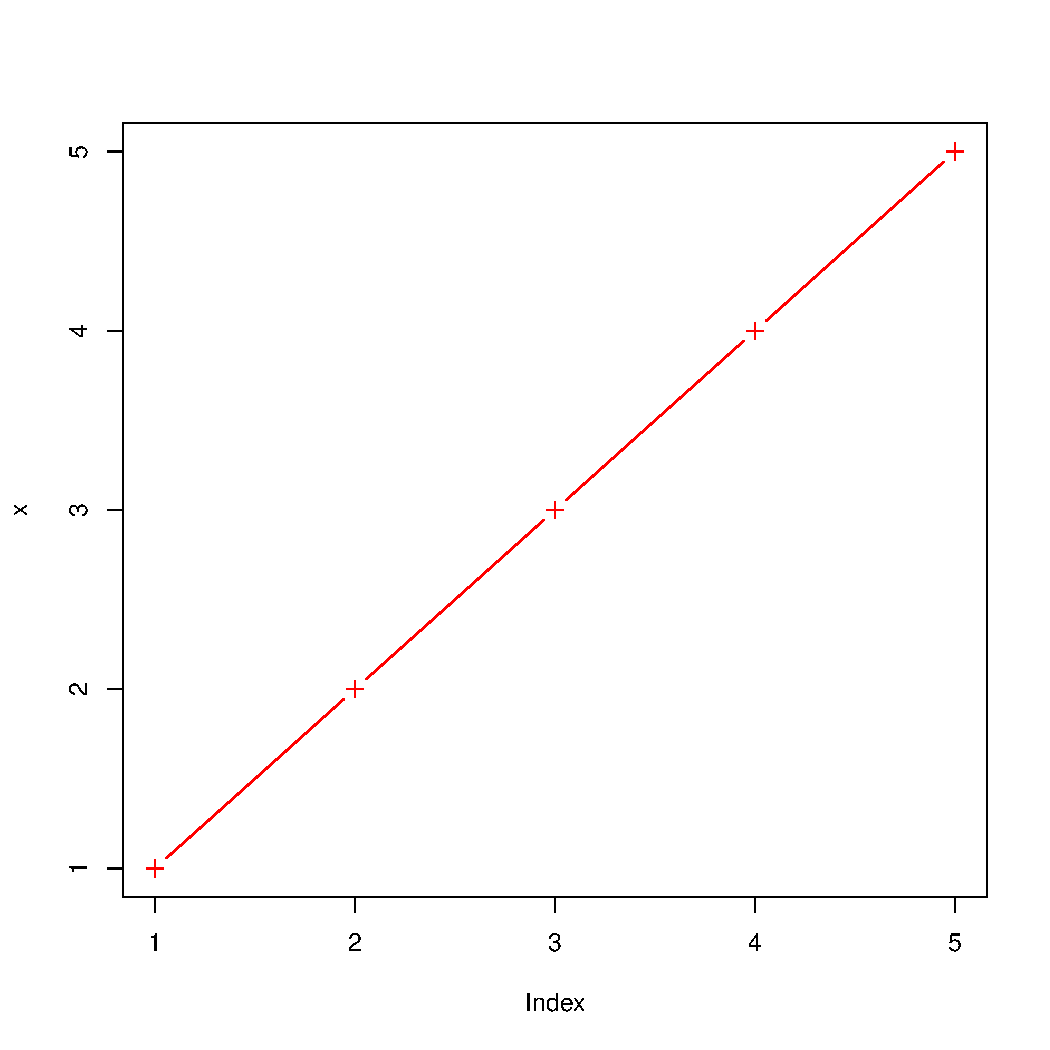
\includegraphics[width=\maxwidth]{figure/unnamed-chunk-101-1} 
\end{knitrout}

Aquí, col y type que no se han especificado en f0, se pasan directamente a la función. Como plot acepta muchos argumentos adicionales, no es necesario especificar todos, si no que se pueden poner \ldots.

\begin{knitrout}
\definecolor{shadecolor}{rgb}{0.969, 0.969, 0.969}\color{fgcolor}\begin{kframe}
\begin{alltt}
\hldef{fa} \hlkwb{<-} \hlkwa{function}\hldef{(}\hlkwc{x}\hldef{,} \hlkwc{col} \hldef{=} \hlsng{"red"}\hldef{,} \hlkwc{...}\hldef{) \{}\hlkwd{plot}\hldef{(x,} \hlkwc{col} \hldef{= col, ...)\}}
\hlkwd{fa}\hldef{(}\hlnum{1}\hlopt{:}\hlnum{5}\hldef{,} \hlsng{"blue"}\hldef{,} \hlkwc{pch} \hldef{=} \hlnum{8}\hldef{)}

\hldef{fb} \hlkwb{<-} \hlkwa{function}\hldef{(}\hlkwc{x}\hldef{,} \hlkwc{col} \hldef{=} \hlsng{"red"}\hldef{,} \hlkwc{...}\hldef{) \{}\hlkwd{plot}\hldef{(x,} \hlkwc{col} \hldef{= col)\}}
\hlkwd{fb}\hldef{(}\hlnum{1}\hlopt{:}\hlnum{5}\hldef{,} \hlsng{"blue"}\hldef{,} \hlkwc{pch} \hldef{=} \hlnum{8}\hldef{)}

\hldef{fc} \hlkwb{<-} \hlkwa{function}\hldef{(}\hlkwc{x}\hldef{,} \hlkwc{col} \hldef{=} \hlsng{"red"}\hldef{) \{}\hlkwd{plot}\hldef{(x,} \hlkwc{col} \hldef{= col, ...)\}}
\hlkwd{fc}\hldef{(}\hlnum{1}\hlopt{:}\hlnum{5}\hldef{,} \hlsng{"blue"}\hldef{,} \hlkwc{pch} \hldef{=} \hlnum{8}\hldef{)}
\end{alltt}
\end{kframe}
\end{knitrout}
La función fa recoge pch dentro de los tres puntos. Además, el color se sobrescribe (el plot resultante tiene los puntos en azul). Tanto fb como fc no hacen lo que se espera, ya que les falta \ldots en la función y en el plot respectivamente. Esa ausencia hace que las funciones no hagan nada con ese argumento.

\section{local}
La función \code{local} permite crear un entorno local en el que trabajar y luego, al salir, que no tenga guardado el valor de las variables.

\begin{knitrout}
\definecolor{shadecolor}{rgb}{0.969, 0.969, 0.969}\color{fgcolor}\begin{kframe}
\begin{alltt}
\hldef{i} \hlkwb{<-} \hlnum{2}
\hlkwd{local}\hldef{(\{}\hlkwd{cat}\hldef{(}\hlsng{"i "}\hldef{, i); i} \hlkwb{<-} \hlnum{99}\hldef{;} \hlkwd{cat}\hldef{(}\hlsng{";  i = "}\hldef{, i)\})}
\end{alltt}
\begin{verbatim}
## i  2;  i =  99
\end{verbatim}
\begin{alltt}
\hldef{i}
\end{alltt}
\begin{verbatim}
## [1] 2
\end{verbatim}
\begin{alltt}
\hlkwd{try}\hldef{(}\hlkwd{rm}\hldef{(vv))}
\hlkwd{local}\hldef{(\{vv} \hlkwb{<-} \hlnum{99}\hldef{;} \hlkwd{cat}\hldef{(}\hlsng{"vv = "}\hldef{, vv)\})}
\end{alltt}
\begin{verbatim}
## vv =  99
\end{verbatim}
\begin{alltt}
\hlkwd{try}\hldef{(vv)}
\end{alltt}
\begin{verbatim}
## Error in eval(expr, envir) : objeto 'vv' no encontrado
\end{verbatim}
\end{kframe}
\end{knitrout}

\section{Evaluación vaga}
La siguiente función toma 2 argumentos, pero solo utiliza 1. Por ello, cuando solo se le pasa un argumento, no se produce ningún error.
\begin{knitrout}
\definecolor{shadecolor}{rgb}{0.969, 0.969, 0.969}\color{fgcolor}\begin{kframe}
\begin{alltt}
\hldef{flazy} \hlkwb{<-} \hlkwa{function}\hldef{(}\hlkwc{x}\hldef{,} \hlkwc{y}\hldef{) \{}\hlkwd{return}\hldef{(}\hlnum{2} \hlopt{*} \hldef{x)\}}
\hlkwd{flazy}\hldef{(}\hlnum{4}\hldef{)}
\end{alltt}
\begin{verbatim}
## [1] 8
\end{verbatim}
\end{kframe}
\end{knitrout}

Esto no es algo a hacer de forma habitual, pero es importante entender por qué el código no se rompe. En otras palabras, la evaluación vaga es la evaluación de los valores cuando se van a utilizar, no cuando se definen.

\chapter{Debugging y capturar excepciones}
Debugging consiste en recorrer el código para comprobar que funciona como se espera y no se estropee. 

\section{\code{traceback}}
\code{traceback} muestra la última llamada y ayuda a identificar dónde se rompió el código para ver qué función tiene un problema. 

\begin{knitrout}
\definecolor{shadecolor}{rgb}{0.969, 0.969, 0.969}\color{fgcolor}\begin{kframe}
\begin{alltt}
\hldef{f1} \hlkwb{<-} \hlkwa{function}\hldef{(}\hlkwc{x}\hldef{)} \hlnum{3} \hlopt{*} \hldef{x}

\hldef{f2} \hlkwb{<-} \hlkwa{function}\hldef{(}\hlkwc{x}\hldef{)} \hlnum{5} \hlopt{+} \hlkwd{f1}\hldef{(x)}

\hldef{f3} \hlkwb{<-} \hlkwa{function}\hldef{(}\hlkwc{z}\hldef{,} \hlkwc{u}\hldef{) \{}
    \hldef{v} \hlkwb{<-} \hlkwd{runif}\hldef{(z)}
    \hldef{a} \hlkwb{<-} \hlkwd{f2}\hldef{(u)}
    \hldef{b} \hlkwb{<-} \hlkwd{f2}\hldef{(}\hlnum{3} \hlopt{*} \hldef{v)}
    \hlkwd{return}\hldef{(a} \hlopt{+} \hldef{b)}
\hldef{\}}

\hlkwd{f3}\hldef{(}\hlnum{3}\hldef{,} \hlnum{7}\hldef{)}
\end{alltt}
\begin{verbatim}
## [1] 36.97035 35.67900 33.98585
\end{verbatim}
\begin{alltt}
\hlkwd{f3}\hldef{(}\hlopt{-}\hlnum{5}\hldef{,} \hlnum{6}\hldef{)}
\end{alltt}


{\ttfamily\noindent\bfseries\color{errorcolor}{\#\# Error in runif(z): invalid arguments}}\begin{alltt}
\hlkwd{traceback}\hldef{()}
\end{alltt}
\begin{verbatim}
## No traceback available
\end{verbatim}
\begin{alltt}
\hlkwd{f3}\hldef{(}\hlnum{5}\hldef{,} \hlsng{"a"}\hldef{)}
\end{alltt}


{\ttfamily\noindent\bfseries\color{errorcolor}{\#\# Error in 3 * x: argumento no-numérico para operador binario}}\begin{alltt}
\hlkwd{traceback}\hldef{()}
\end{alltt}
\begin{verbatim}
## No traceback available
\end{verbatim}
\end{kframe}
\end{knitrout}

\section{\code{debug} and \code{browser}}
El comando \code{debug} permite ir paso a paso ejecutando cada línea del código. Cuando se quiera parar, hay que poner simplemente \code{undebug}.

\begin{knitrout}
\definecolor{shadecolor}{rgb}{0.969, 0.969, 0.969}\color{fgcolor}\begin{kframe}
\begin{alltt}
\hlkwd{debug}\hldef{(f3)}
\hlkwd{f3}\hldef{(}\hlnum{3}\hldef{,} \hlnum{5}\hldef{)}
\hlkwd{undebug}\hldef{(f3)} \hlcom{## stop debugging}
\hlkwd{f3}\hldef{(}\hlnum{3}\hldef{,} \hlnum{5}\hldef{)}
\end{alltt}
\end{kframe}
\end{knitrout}

El comando \code{browser} para la ejecución de la expresión actual y permite acceder al intérprete de R. También se puede realizar de forma condicional.

\begin{knitrout}
\definecolor{shadecolor}{rgb}{0.969, 0.969, 0.969}\color{fgcolor}\begin{kframe}
\begin{alltt}
\hlcom{## just browser}
\hldef{f3} \hlkwb{<-} \hlkwa{function}\hldef{(}\hlkwc{z}\hldef{,} \hlkwc{u}\hldef{) \{}
    \hldef{v} \hlkwb{<-} \hlkwd{runif}\hldef{(z)}
    \hldef{a} \hlkwb{<-} \hlkwd{f2}\hldef{(u)}
    \hlkwd{browser}\hldef{()}
    \hldef{b} \hlkwb{<-} \hlkwd{f2}\hldef{(}\hlnum{3} \hlopt{*} \hldef{v)}
    \hlkwd{return}\hldef{(a} \hlopt{+} \hldef{b)}
\hldef{\}}

\hlcom{## with conditional browser}
\hldef{f3} \hlkwb{<-} \hlkwa{function}\hldef{(}\hlkwc{z}\hldef{,} \hlkwc{u}\hldef{) \{}
    \hldef{v} \hlkwb{<-} \hlkwd{runif}\hldef{(z)}
    \hlkwa{if} \hldef{(z} \hlopt{>} \hlnum{5}\hldef{)} \hlkwd{browser}\hldef{()}
    \hldef{a} \hlkwb{<-} \hlkwd{f2}\hldef{(u)}
    \hldef{b} \hlkwb{<-} \hlkwd{f2}\hldef{(}\hlnum{3} \hlopt{*} \hldef{v)}
    \hlkwd{return}\hldef{(a} \hlopt{+} \hldef{b)}
\hldef{\}}
\end{alltt}
\end{kframe}
\end{knitrout}

Desde \code{browser}, hay una serie de expresiones:
\begin{itemize}
\item n o enter permite ejecutar la siguiente línea.
\item c: salir del browser y continuar la ejecución del siguiente statement.
\item s: evalúa el siguiente statement entrando en las siguientes funciones.
\item Q: salir de la evaluación actual e ir al sitio desde donde se llamó.
\end{itemize}

\code{debug} es como poner \code{browser} al inicio del código.

\section{\code{trace} para ver funciones arbitrarias en sitios arbitrarios}
Se puede utilizar \code{debug} con funciones que no hayamos escrito nosotros (por ejemplo, \code{debug(lm)}). Sin embargo, la función lm es muy larga y quizás no queremos empezar por arriba, si no que sospechamos que nuestros problemas están por el medio. Para eso, podemos utilizar \code{trace}.

\begin{knitrout}
\definecolor{shadecolor}{rgb}{0.969, 0.969, 0.969}\color{fgcolor}\begin{kframe}
\begin{alltt}
\hlkwd{trace}\hldef{(}\hlsng{"lm"}\hldef{,} \hlkwc{edit} \hldef{=} \hlnum{TRUE}\hldef{)}
\end{alltt}
\end{kframe}
\end{knitrout}

\begin{knitrout}
\definecolor{shadecolor}{rgb}{0.969, 0.969, 0.969}\color{fgcolor}\begin{kframe}
\begin{alltt}
\hlkwd{as.list}\hldef{(}\hlkwd{body}\hldef{(lm))}
\hlkwd{trace}\hldef{(lm,} \hlkwc{tracer} \hldef{= browser,} \hlkwc{at} \hldef{=} \hlnum{5}\hldef{)}
\hldef{y} \hlkwb{<-} \hlkwd{runif}\hldef{(}\hlnum{100}\hldef{)}
\hldef{x} \hlkwb{<-} \hlnum{1}\hlopt{:}\hlnum{100}
\hlkwd{lm}\hldef{(y} \hlopt{~} \hldef{x)}
\hlcom{## stop tracing}
\hlkwd{untrace}\hldef{(lm)}
\end{alltt}
\end{kframe}
\end{knitrout}

\section{Warnings}
En R puede haber algunas funciones que no den error, pero muestren warnings. En algunos casos, los warnings pueden indicar que algo no esté funcionando, por lo que se pueden convertir los warnings en errores para que la función no se ejecute. 

\begin{knitrout}
\definecolor{shadecolor}{rgb}{0.969, 0.969, 0.969}\color{fgcolor}\begin{kframe}
\begin{alltt}
\hldef{opt} \hlkwb{<-} \hlkwd{options}\hldef{(}\hlkwc{warn} \hldef{=} \hlnum{2}\hldef{)}
\end{alltt}
\end{kframe}
\end{knitrout}

Este código hace que los warnings se comporten como errores. Una vez terminado, se puede reestablecer a los valores predeterminados mediante:

\begin{knitrout}
\definecolor{shadecolor}{rgb}{0.969, 0.969, 0.969}\color{fgcolor}\begin{kframe}
\begin{alltt}
\hlkwd{options}\hldef{(opt)}
\end{alltt}
\end{kframe}
\end{knitrout}

\section{\code{where} para cuando uno está perdido en dónde está}
A veces, cuando se hace debugging, especialmente cuando se está dentro de varias funciones que se llaman unas a otras, uno puede perderse y no saber dónde está. En estos casos, se utiliza \code{where}, que devuelve la función en la que nos encontramos.

\begin{knitrout}
\definecolor{shadecolor}{rgb}{0.969, 0.969, 0.969}\color{fgcolor}\begin{kframe}
\begin{alltt}
\hlkwd{debug}\hldef{(f1);} \hlkwd{debug}\hldef{(f2);} \hlkwd{debug}\hldef{(f3)}
\hlkwd{f3}\hldef{(}\hlnum{4}\hldef{,} \hlnum{5}\hldef{)} \hlcom{## now, keeping pressing enter or n}
         \hlcom{## and you'll get deeper and deeper}
         \hlcom{## while in browser mode, type where}

\hlcom{#Return things to normal}
\hlkwd{undebug}\hldef{(f3)}
\hlkwd{undebug}\hldef{(f2)}
\hlkwd{undebug}\hldef{(f1)}
\end{alltt}
\end{kframe}
\end{knitrout}

%04/11 - Ramón
\section{Protección frente a posibles fallos}
Hay un manejo excepcional en R mediante \code{try}. Esto permite evitar que el código no falle. Cuando se va a dar un error, la variable adquiere la clase try-error.

\begin{knitrout}
\definecolor{shadecolor}{rgb}{0.969, 0.969, 0.969}\color{fgcolor}\begin{kframe}
\begin{alltt}
\hldef{ft} \hlkwb{<-} \hlkwa{function}\hldef{(}\hlkwc{x}\hldef{) \{}
    \hldef{tmp} \hlkwb{<-} \hlkwd{try}\hldef{(}\hlkwd{log}\hldef{(x),} \hlkwc{silent} \hldef{=} \hlnum{TRUE}\hldef{)}
    \hlkwa{if}\hldef{(}\hlkwd{inherits}\hldef{(tmp,} \hlsng{"try-error"}\hldef{)) \{}
        \hlkwd{warning}\hldef{(}\hlkwd{paste}\hldef{(}\hlsng{"It looks like something did not work:\textbackslash{}n"}\hldef{,}
                      \hlsng{"   "}\hldef{, tmp))}
    \hldef{\}} \hlkwa{else}\hldef{\{}
        \hlkwd{return}\hldef{(tmp)}
    \hldef{\}}
\hldef{\}}

\hlkwd{ft}\hldef{(}\hlnum{9}\hldef{)}
\end{alltt}
\begin{verbatim}
## [1] 2.197225
\end{verbatim}
\begin{alltt}
\hlkwd{ft}\hldef{(}\hlsng{"a"}\hldef{)}
\end{alltt}


{\ttfamily\noindent\color{warningcolor}{\#\# Warning in ft("{}a"{}): It looks like something did not work:\\\#\# \ \ \ \ \ Error in log(x) : Argumento no numérico para una función matemática}}\end{kframe}
\end{knitrout}

\section{Funciones de debugging que no son exportadas}
Si cargamos un paquete, sirve con \code{library(paquete)}. No obstante, puede haber algunas funciones no exportadas (no se ve directamente al teclear el nombre).

\begin{knitrout}
\definecolor{shadecolor}{rgb}{0.969, 0.969, 0.969}\color{fgcolor}\begin{kframe}
\begin{alltt}
\hlkwd{trace}\hldef{(randomForest}\hlopt{:::}\hldef{predict.randomForest,} \hlkwc{edit} \hldef{=} \hlnum{TRUE}\hldef{)}
\end{alltt}
\end{kframe}
\end{knitrout}

Las \textbf{funciones exportadas} son aquellas que el paquete pone a disposición del usuario final. Esto significa que cualquier persona que cargue el paquete puede llamar a estas funciones directamente. Así, cuando la función está exportada, el usuario solo necesita escribir el nombre de la función para ejecutarla, siempre que el paquete esté cargado.

Las \textbf{funciones no exportadas} son aquellas que están presentes en el paquete pero no están pensadas para ser utilizadas por el usuario final. Estas funciones suelen ser de uso interno, y los desarrolladores del paquete las utilizan para realizar tareas auxiliares o para construir las funciones exportadas de manera modular. No aparecen en la lista de funciones del paquete y no son accesibles directamente.

\chapter{Programación orientada a objetos: clases S3 y S4}
En R hay varios sistemas de programación orientada a objetos. Los sistemas originales en R son los sistemas S3 y S4, siendo los más extendidos. 

\section{\code{methods}}
\begin{knitrout}
\definecolor{shadecolor}{rgb}{0.969, 0.969, 0.969}\color{fgcolor}\begin{kframe}
\begin{alltt}
\hlkwd{methods}\hldef{(}\hlsng{'plot'}\hldef{)}
\hlkwd{getAnywhere}\hldef{(plot.TukeyHSD)}
\hlcom{#stats:::plot.TukeyHSD}
\end{alltt}
\end{kframe}
\end{knitrout}

\code{getAnywhere} permite obtener las funciones no exportadas. \code{plot} realmente no hace nada, solo determina el tipo de objeto que se le ha pasado y llama a la función específica para ese objeto.

Lo que se ve con \code{methods} depende de los paquetes que haya cargados y, por tanto, lo que haya en nuestro espacio de búsqueda. 

En POO en R, no se define una clase dentro de la que definir métodos (como en Python). Los métodos no pertenecen a la clase, si no que hay que definirlos por separado. 

Se pueden buscar todos los métodos de una clase con:
\begin{knitrout}
\definecolor{shadecolor}{rgb}{0.969, 0.969, 0.969}\color{fgcolor}\begin{kframe}
\begin{alltt}
\hlkwd{methods}\hldef{(}\hlkwc{class} \hldef{=} \hlsng{'lm'}\hldef{)}
\hlkwd{methods}\hldef{(}\hlkwc{class} \hldef{=} \hlsng{'lm'}\hldef{,} \hlkwc{byclass} \hldef{=} \hlnum{FALSE}\hldef{)}
\end{alltt}
\end{kframe}
\end{knitrout}

El argumento \code{byclass} muestra el nombre completo de los métodos y si están o no exportados. 

El código fuente de todas las funciones está disponible. Para todas las funciones S3 exportadas desde el namespace, se puede escribir el nombre del método en la línea de comando como generic.class. Para las funciones no exportadas, se puede utilizar \code{getAnywhere} o \code{getS3method}. Sabiendo el namespace, también se puede utilizar :::. 

\begin{knitrout}
\definecolor{shadecolor}{rgb}{0.969, 0.969, 0.969}\color{fgcolor}\begin{kframe}
\begin{alltt}
\hldef{add1.lm}
\hlkwd{getAnywhere}\hldef{(}\hlsng{'add1.lm'}\hldef{)}
\hldef{stats}\hlopt{:::}\hldef{add1.lm}
\hlkwd{getS3method}\hldef{(}\hlsng{'add1'}\hldef{,} \hlsng{'lm'}\hldef{)}
\end{alltt}
\end{kframe}
\end{knitrout}

\section{Creación de clases y métodos}
Vamos a suponer que queremos trabajar con unos data frames especiales con información sobre colesterol, la expresión de un gen y el tipo de experimento que lo midió. Lo primero que se quiere es convertir data frames en objetos de mi clase (y más adelante convertir matrices o vectores a objetos), crear un summary de los objetos y ajustar funciones de plot. Finalmente, hay que testear el código mediante la librería \code{testthat}.

Empezamos con una función genérica de conversión al objeto y luego un método que funcione para los data frames. El objeto será Cholest\_Gene object, por lo que un conversor genérico (y sus comentarios) sería:

\begin{knitrout}
\definecolor{shadecolor}{rgb}{0.969, 0.969, 0.969}\color{fgcolor}\begin{kframe}
\begin{alltt}
\hlcom{# object -> Cholest_Gene object}
\hlcom{# General converter to Cholest_Gene object.}
\hldef{to_CG} \hlkwb{<-} \hlkwa{function}\hldef{(}\hlkwc{x}\hldef{,} \hlkwc{...}\hldef{) \{}
  \hlkwd{UseMethod}\hldef{(}\hlsng{"to_CG"}\hldef{)}
\hldef{\}}
\end{alltt}
\end{kframe}
\end{knitrout}

El primer método será convertir un data frame al objeto:
\begin{knitrout}
\definecolor{shadecolor}{rgb}{0.969, 0.969, 0.969}\color{fgcolor}\begin{kframe}
\begin{alltt}
\hlcom{# data.frame -> Cholest_Gene object}
\hlcom{# Take a data frame and return (if possible) a Cholest_Gene object.}
\hldef{to_CG.data.frame} \hlkwb{<-} \hlkwa{function}\hldef{(}\hlkwc{x}\hldef{) \{}
  \hldef{cns} \hlkwb{<-} \hlkwd{c}\hldef{(}\hlsng{"Cholesterol"}\hldef{,} \hlsng{"Gene"}\hldef{,} \hlsng{"Kind"}\hldef{)}
  \hlkwa{if} \hldef{(}\hlopt{!}\hldef{(}\hlkwd{all}\hldef{(}\hlkwd{colnames}\hldef{(x)} \hlopt \hldef{cns)))}
        \hlkwd{stop}\hldef{(}\hlkwd{paste}\hldef{(}\hlsng{"Column names are not "}\hldef{, cns))}
    \hldef{tmp} \hlkwb{<-} \hldef{x[, cns]}
    \hlcom{## Notice I do not set this to be of data.frame class}
    \hlkwd{class}\hldef{(tmp)} \hlkwb{<-} \hlkwd{c}\hldef{(}\hlsng{"Cholest_Gene"}\hldef{)}
    \hlkwd{return}\hldef{(tmp)}
\hldef{\}}
\end{alltt}
\end{kframe}
\end{knitrout}

Y se debe probar:
\begin{knitrout}
\definecolor{shadecolor}{rgb}{0.969, 0.969, 0.969}\color{fgcolor}\begin{kframe}
\begin{alltt}
\hldef{uu} \hlkwb{<-} \hlkwd{to_CG}\hldef{(}\hlkwd{data.frame}\hldef{(}\hlkwc{Cholesterol} \hldef{=} \hlnum{1}\hlopt{:}\hlnum{10}\hldef{,} \hlkwc{Gene} \hldef{=} \hlnum{11}\hlopt{:}\hlnum{20}\hldef{,} \hlkwc{Kind} \hldef{=} \hlsng{"Cl1"}\hldef{))}
\hldef{uu}
\end{alltt}
\end{kframe}
\end{knitrout}
El resultado de la visualización es muy feo y se debe mejorar. Esto se debe a que la clase es Cholest\_Gene y, por ello, utiliza print default. Por ello, se debe cambiar la clase del objeto a la clase Cholest\_Gene, adjuntando la clase que tenía previamente:
\begin{knitrout}
\definecolor{shadecolor}{rgb}{0.969, 0.969, 0.969}\color{fgcolor}\begin{kframe}
\begin{alltt}
\hlcom{# data.frame -> Cholest_Gene object}
\hlcom{# Take a data frame and return (if possible) a Cholest_Gene object.}
\hldef{to_CG.data.frame} \hlkwb{<-} \hlkwa{function}\hldef{(}\hlkwc{x}\hldef{) \{}
    \hldef{cns} \hlkwb{<-} \hlkwd{c}\hldef{(}\hlsng{"Cholesterol"}\hldef{,} \hlsng{"Gene"}\hldef{,} \hlsng{"Kind"}\hldef{)}
    \hlkwa{if} \hldef{(}\hlopt{!}\hldef{(}\hlkwd{all}\hldef{(}\hlkwd{colnames}\hldef{(x)} \hlopt \hldef{cns)))}
        \hlkwd{stop}\hldef{(}\hlkwd{paste}\hldef{(}\hlsng{"Column names are not "}\hldef{, cns))}
    \hldef{tmp} \hlkwb{<-} \hldef{x[, cns]}
    \hldef{tmp}\hlopt{$}\hldef{Kind} \hlkwb{<-} \hlkwd{factor}\hldef{(tmp}\hlopt{$}\hldef{Kind)}
    \hlkwd{class}\hldef{(tmp)} \hlkwb{<-} \hlkwd{c}\hldef{(}\hlsng{"Cholest_Gene"}\hldef{,} \hlkwd{class}\hldef{(tmp))} \hlcom{## "data.frame")}
    \hlkwd{return}\hldef{(tmp)}
\hldef{\}}
\end{alltt}
\end{kframe}
\end{knitrout}

De esta forma, la visualización del objeto está bien, al igual que la salida de summary, reutilizando así las funciones existentes.
\begin{knitrout}
\definecolor{shadecolor}{rgb}{0.969, 0.969, 0.969}\color{fgcolor}\begin{kframe}
\begin{alltt}
\hldef{uu} \hlkwb{<-} \hlkwd{to_CG}\hldef{(}\hlkwd{data.frame}\hldef{(}\hlkwc{Cholesterol} \hldef{=} \hlnum{1}\hlopt{:}\hlnum{10}\hldef{,} \hlkwc{Gene} \hldef{=} \hlnum{11}\hlopt{:}\hlnum{20}\hldef{,} \hlkwc{Kind} \hldef{=} \hlsng{"Cl1"}\hldef{))}
\hlkwd{summary}\hldef{(uu)}
\hlkwd{print}\hldef{(uu)}
\hldef{uu}
\end{alltt}
\end{kframe}
\end{knitrout}

La siguiente función es más sofisticada:
\begin{knitrout}
\definecolor{shadecolor}{rgb}{0.969, 0.969, 0.969}\color{fgcolor}\begin{kframe}
\begin{alltt}
\hlcom{# Cholest_Gene object -> printed Cholest_Gene object}
\hlcom{# Print a Cholest_Gene object.}
\hldef{print.Cholest_Gene} \hlkwb{<-} \hlkwa{function}\hldef{(}\hlkwc{x}\hldef{) \{}
    \hldef{u} \hlkwb{<-} \hldef{x[,} \hlkwd{c}\hldef{(}\hlnum{1}\hldef{,} \hlnum{2}\hldef{)]}
    \hlkwd{class}\hldef{(u)} \hlkwb{<-} \hlsng{"data.frame"}
    \hlkwd{print}\hldef{(u)}
    \hlkwd{cat}\hldef{(}\hlsng{"\textbackslash{}n Printing summary of first column \textbackslash{}n"}\hldef{)}
    \hlkwd{print}\hldef{(}\hlkwd{summary}\hldef{(x[,} \hlnum{1}\hldef{]))}
\hldef{\}}
\end{alltt}
\end{kframe}
\end{knitrout}

En este caso, se asigna la clase data.frame (y solo esa clase) para evitar que se llame a sí mismo.

Como por el momento solo se ha creado el método para convertir data frames a nuestro objeto, se debe comprobar que el objeto que se pase sea de una clase soportada (data frame) y no se ejecute cuando la clase (por ejemplo, matriz) no está soportada. Además, esto muestra un mensaje de error personalizado.
\begin{knitrout}
\definecolor{shadecolor}{rgb}{0.969, 0.969, 0.969}\color{fgcolor}\begin{kframe}
\begin{alltt}
\hlcom{# arbitrary object -> failure message if no method}
\hlcom{# Return error message if there is no specific method to convert }
\hlcom{# from that class to Cholest_Gene class}
\hldef{to_CG.default} \hlkwb{<-} \hlkwa{function}\hldef{(}\hlkwc{x}\hldef{) \{}
    \hlkwd{stop}\hldef{(}\hlsng{"For now, only methods for data.frame are available."}\hldef{)}
\hldef{\}}
\end{alltt}
\end{kframe}
\end{knitrout}

\section{Testeo y test-driven development}
El último paso es el testeo, y es algo fundamental. En los tests se van poniendo casos en los que se encuentran bugs y se arreglan. Como mínimo, se debe comprobar que se puede crear un objeto legítimo de un data frame, que falla (como esperamos) cuando al data frame le faltan columnas y que falla (como esperamos) cuando no se proporciona un data frame. El testeo se puede llevar a cabo con el paquete \code{testthat}, el cual tiene varios bloques de salidas que se pueden esperar (\code{expect\_s3\_class, expect\_error, expect\_equal, ...})

\begin{knitrout}
\definecolor{shadecolor}{rgb}{0.969, 0.969, 0.969}\color{fgcolor}\begin{kframe}
\begin{alltt}
\hlkwd{library}\hldef{(testthat)}
\hlkwd{test_that}\hldef{(}\hlsng{"minimal conversions and failures"}\hldef{, \{}

    \hlkwd{expect_s3_class}\hldef{(}\hlkwd{to_CG}\hldef{(}\hlkwd{data.frame}\hldef{(}\hlkwc{Cholesterol} \hldef{=} \hlnum{1}\hlopt{:}\hlnum{10}\hldef{,} \hlkwc{Gene} \hldef{=} \hlnum{11}\hlopt{:}\hlnum{20}\hldef{,}
                                     \hlkwc{Kind} \hldef{=} \hlsng{"Cl1"}\hldef{)),} \hlsng{"Cholest_Gene"}\hldef{)}


    \hlkwd{expect_error}\hldef{(}\hlkwd{to_CG}\hldef{(}\hlkwd{cbind}\hldef{(}\hlkwc{Cholesterol} \hldef{=} \hlnum{1}\hlopt{:}\hlnum{10}\hldef{,} \hlkwc{Gene} \hldef{=} \hlnum{11}\hlopt{:}\hlnum{20}\hldef{)),}
                 \hlsng{"For now, only methods for data.frame are available"}\hldef{,}
                 \hlkwc{fixed} \hldef{=} \hlnum{TRUE}\hldef{)}

    \hlkwd{expect_error}\hldef{(}\hlkwd{to_CG}\hldef{(}\hlkwd{data.frame}\hldef{(}\hlkwc{Cholesterol} \hldef{=} \hlnum{1}\hlopt{:}\hlnum{10}\hldef{,} \hlkwc{Geni} \hldef{=} \hlnum{11}\hlopt{:}\hlnum{20}\hldef{,}
                                     \hlkwc{Kind} \hldef{=} \hlsng{"Cl1"}\hldef{)),}
                 \hlsng{"Column names are not "}\hldef{,}
                 \hlkwc{fixed} \hldef{=} \hlnum{TRUE}\hldef{)}

    \hlkwd{expect_s3_class}\hldef{(}\hlkwd{to_CG}\hldef{(}\hlkwd{data.frame}\hldef{(}\hlkwc{Cholesterol} \hldef{=} \hlnum{1}\hlopt{:}\hlnum{10}\hldef{,} \hlkwc{Gene} \hldef{=} \hlnum{11}\hlopt{:}\hlnum{20}\hldef{,}
                                     \hlkwc{Kind} \hldef{=} \hlsng{"Cl1"}\hldef{,}
                                     \hlkwc{whatever} \hldef{=} \hlsng{"abcd"}\hldef{)),}
                    \hlsng{"Cholest_Gene"}\hldef{)}

\hldef{\})}
\end{alltt}
\end{kframe}
\end{knitrout}

El último bloque de test ha fallado, por lo que hay que hacer debugging. 
\begin{knitrout}
\definecolor{shadecolor}{rgb}{0.969, 0.969, 0.969}\color{fgcolor}\begin{kframe}
\begin{alltt}
\hlkwd{debugonce}\hldef{(to_CG.data.frame)}

\hldef{dummy} \hlkwb{<-} \hlkwd{to_CG}\hldef{(}\hlkwd{data.frame}\hldef{(}\hlkwc{Cholesterol} \hldef{=} \hlnum{1}\hlopt{:}\hlnum{10}\hldef{,} \hlkwc{Gene} \hldef{=} \hlnum{11}\hlopt{:}\hlnum{20}\hldef{,}
                                 \hlkwc{Kind} \hldef{=} \hlsng{"Cl1"}\hldef{,}
                                 \hlkwc{whatever} \hldef{=} \hlsng{"abcd"}\hldef{))}
\end{alltt}
\end{kframe}
\end{knitrout}

En este entorno se va viendo qué va pasando en cada línea de código, y se verifica dónde está el problema. En este caso, el if comprueba si todos los nombres de columnas están en cns, cuando debería ser al revés: que todos los nombres de cns estén en el data frame (aunque haya otras columnas adicionales). Por tanto, hay que reescribir la función invirtiendo eso:

\begin{knitrout}
\definecolor{shadecolor}{rgb}{0.969, 0.969, 0.969}\color{fgcolor}\begin{kframe}
\begin{alltt}
\hldef{to_CG.data.frame} \hlkwb{<-} \hlkwa{function}\hldef{(}\hlkwc{x}\hldef{) \{}
    \hldef{cns} \hlkwb{<-} \hlkwd{c}\hldef{(}\hlsng{"Cholesterol"}\hldef{,} \hlsng{"Gene"}\hldef{,} \hlsng{"Kind"}\hldef{)}
    \hlkwa{if} \hldef{(}\hlopt{!}\hldef{(}\hlkwd{all}\hldef{(cns} \hlopt \hlkwd{colnames}\hldef{(x))))}
        \hlkwd{stop}\hldef{(}\hlkwd{paste}\hldef{(}\hlsng{"Column names are not "}\hldef{,}
                   \hlkwd{paste}\hldef{(cns,} \hlkwc{collapse} \hldef{=} \hlsng{" "}\hldef{)))}
    \hldef{tmp} \hlkwb{<-} \hldef{x[, cns]}
    \hldef{tmp}\hlopt{$}\hldef{Kind} \hlkwb{<-} \hlkwd{factor}\hldef{(tmp}\hlopt{$}\hldef{Kind)}
    \hlkwd{class}\hldef{(tmp)} \hlkwb{<-} \hlkwd{c}\hldef{(}\hlsng{"Cholest_Gene"}\hldef{,} \hlkwd{class}\hldef{(x))}
    \hlkwd{return}\hldef{(tmp)}
\hldef{\}}
\end{alltt}
\end{kframe}
\end{knitrout}

Y volvemos a ejecutar el bloque de comprobaciones:
\begin{knitrout}
\definecolor{shadecolor}{rgb}{0.969, 0.969, 0.969}\color{fgcolor}\begin{kframe}
\begin{alltt}
\hlkwd{test_that}\hldef{(}\hlsng{"minimal conversions and failures"}\hldef{, \{}
    \hlkwd{expect_s3_class}\hldef{(}\hlkwd{to_CG}\hldef{(}\hlkwd{data.frame}\hldef{(}\hlkwc{Cholesterol} \hldef{=} \hlnum{1}\hlopt{:}\hlnum{10}\hldef{,}
                                     \hlkwc{Gene} \hldef{=} \hlnum{11}\hlopt{:}\hlnum{20}\hldef{,}
                                     \hlkwc{Kind} \hldef{=} \hlsng{"Cl1"}\hldef{)),}
                    \hlsng{"Cholest_Gene"}\hldef{)}
    \hlkwd{expect_error}\hldef{(}\hlkwd{to_CG}\hldef{(}\hlkwd{cbind}\hldef{(}\hlkwc{Cholesterol} \hldef{=} \hlnum{1}\hlopt{:}\hlnum{10}\hldef{,} \hlkwc{Gene} \hldef{=} \hlnum{11}\hlopt{:}\hlnum{20}\hldef{)),}
                 \hlsng{"For now, only methods for data.frame are available"}\hldef{,}
                 \hlkwc{fixed} \hldef{=} \hlnum{TRUE}\hldef{)}
    \hlkwd{expect_error}\hldef{(}\hlkwd{to_CG}\hldef{(}\hlkwd{data.frame}\hldef{(}\hlkwc{Cholesterol} \hldef{=} \hlnum{1}\hlopt{:}\hlnum{10}\hldef{,} \hlkwc{Geni} \hldef{=} \hlnum{11}\hlopt{:}\hlnum{20}\hldef{,}
                                  \hlkwc{Kind} \hldef{=} \hlsng{"Cl1"}\hldef{)),}
                 \hlsng{"Column names are not"}\hldef{,}
                 \hlkwc{fixed} \hldef{=} \hlnum{TRUE}\hldef{)}
    \hlkwd{expect_s3_class}\hldef{(}\hlkwd{to_CG}\hldef{(}\hlkwd{data.frame}\hldef{(}\hlkwc{Cholesterol} \hldef{=} \hlnum{1}\hlopt{:}\hlnum{10}\hldef{,} \hlkwc{Gene} \hldef{=} \hlnum{11}\hlopt{:}\hlnum{20}\hldef{,}
                                     \hlkwc{Kind} \hldef{=} \hlsng{"Cl1"}\hldef{,}
                                     \hlkwc{whatever} \hldef{=} \hlsng{"abcd"}\hldef{)),} \hlsng{"Cholest_Gene"}\hldef{)}
\hldef{\})}
\end{alltt}
\end{kframe}
\end{knitrout}

\section{Creación de función de plot}
\begin{knitrout}
\definecolor{shadecolor}{rgb}{0.969, 0.969, 0.969}\color{fgcolor}\begin{kframe}
\begin{alltt}
\hlcom{## Cholest_Gene object -> ggplot object}
\hlcom{## Produce a ggplot of a Cholest_Gene object.}
\hldef{plot.Cholest_Gene} \hlkwb{<-} \hlkwa{function}\hldef{(}\hlkwc{x}\hldef{,} \hlkwc{...}\hldef{) \{}
  \hlkwd{class}\hldef{(x)} \hlkwb{<-} \hlsng{"data.frame"}
  \hlkwd{require}\hldef{(ggplot2)}
  \hlcom{## FIXME: should I explicitly print? Hummm.. return, as orthodox?}
  \hlkwa{if} \hldef{(}\hlkwd{nlevels}\hldef{(x}\hlopt{$}\hldef{Kind)} \hlopt{>=} \hlnum{2}\hldef{)}
    \hldef{p1} \hlkwb{<-} \hlkwd{ggplot}\hldef{(}\hlkwd{aes}\hldef{(}\hlkwc{y} \hldef{= Cholesterol,} \hlkwc{x} \hldef{= Gene,} \hlkwc{col} \hldef{= Kind),}
                 \hlkwc{data} \hldef{= x)} \hlopt{+}
      \hlkwd{facet_grid}\hldef{(}\hlopt{~} \hldef{Kind)}
  \hlkwa{else}
    \hldef{p1} \hlkwb{<-} \hlkwd{ggplot}\hldef{(}\hlkwd{aes}\hldef{(}\hlkwc{y} \hldef{= Cholesterol,} \hlkwc{x} \hldef{= Gene),} \hlkwc{data} \hldef{= x)}
  \hldef{p1} \hlkwb{<-} \hldef{p1} \hlopt{+} \hlkwd{geom_point}\hldef{()}
  \hlkwd{return}\hldef{(p1)}
\hldef{\}}
\end{alltt}
\end{kframe}
\end{knitrout}

En R, cuando se pasa un argumento, tan pronto como se utiliza en el interior de la función, se hace una copia. Así, cuando se modifica la clase dentro de una función, no se altera el argumento original, solo la copia interna. 

\section{Clases S4}
Las clases S4 se utilizan en algunos paquetes de BioConductor. Funcionan de forma similar a las clases S3, pero son más formales y rigurosas. 

\begin{knitrout}
\definecolor{shadecolor}{rgb}{0.969, 0.969, 0.969}\color{fgcolor}\begin{kframe}
\begin{alltt}
\hlkwd{library}\hldef{(Matrix)}
\hldef{m1} \hlkwb{<-} \hlkwd{Matrix}\hldef{(}\hlnum{1}\hlopt{:}\hlnum{9}\hldef{,} \hlkwc{nrow} \hldef{=} \hlnum{3}\hldef{)}
\hldef{m2} \hlkwb{<-} \hlkwd{Diagonal}\hldef{(}\hlnum{5}\hldef{)}

\hldef{x} \hlkwb{<-} \hlnum{0}\hlopt{:}\hlnum{10}
\hldef{y} \hlkwb{<-} \hlkwd{c}\hldef{(}\hlnum{26}\hldef{,} \hlnum{17}\hldef{,} \hlnum{13}\hldef{,} \hlnum{12}\hldef{,} \hlnum{20}\hldef{,} \hlnum{5}\hldef{,} \hlnum{9}\hldef{,} \hlnum{8}\hldef{,} \hlnum{5}\hldef{,} \hlnum{4}\hldef{,} \hlnum{8}\hldef{)}
\hldef{fit1} \hlkwb{<-} \hlkwd{lm}\hldef{(y} \hlopt{~} \hldef{x)}

\hlkwd{class}\hldef{(fit1)}
\end{alltt}
\begin{verbatim}
## [1] "lm"
\end{verbatim}
\begin{alltt}
\hlkwd{is.list}\hldef{(fit1)}
\end{alltt}
\begin{verbatim}
## [1] TRUE
\end{verbatim}
\begin{alltt}
\hlkwd{isS4}\hldef{(fit1)}
\end{alltt}
\begin{verbatim}
## [1] FALSE
\end{verbatim}
\begin{alltt}
\hlkwd{print}\hldef{(fit1)}
\end{alltt}
\begin{verbatim}
## 
## Call:
## lm(formula = y ~ x)
## 
## Coefficients:
## (Intercept)            x  
##      19.955       -1.682
\end{verbatim}
\begin{alltt}
\hldef{stats}\hlopt{:::}\hlkwd{print.lm}\hldef{(fit1)}
\end{alltt}
\begin{verbatim}
## 
## Call:
## lm(formula = y ~ x)
## 
## Coefficients:
## (Intercept)            x  
##      19.955       -1.682
\end{verbatim}
\begin{alltt}
\hldef{fit1}
\end{alltt}
\begin{verbatim}
## 
## Call:
## lm(formula = y ~ x)
## 
## Coefficients:
## (Intercept)            x  
##      19.955       -1.682
\end{verbatim}
\begin{alltt}
\hlkwd{names}\hldef{(fit1)}
\end{alltt}
\begin{verbatim}
##  [1] "coefficients"  "residuals"     "effects"      
##  [4] "rank"          "fitted.values" "assign"       
##  [7] "qr"            "df.residual"   "xlevels"      
## [10] "call"          "terms"         "model"
\end{verbatim}
\begin{alltt}
\hldef{fit1}\hlopt{$}\hldef{coefficients}
\end{alltt}
\begin{verbatim}
## (Intercept)           x 
##   19.954545   -1.681818
\end{verbatim}
\begin{alltt}
\hlcom{## don't do that for real. Use coefficients}
\hlkwd{coefficients}\hldef{(fit1)}
\end{alltt}
\begin{verbatim}
## (Intercept)           x 
##   19.954545   -1.681818
\end{verbatim}
\begin{alltt}
\hlkwd{isS4}\hldef{(m1)}
\end{alltt}
\begin{verbatim}
## [1] TRUE
\end{verbatim}
\begin{alltt}
\hlkwd{is.list}\hldef{(m1)}
\end{alltt}
\begin{verbatim}
## [1] FALSE
\end{verbatim}
\begin{alltt}
\hlkwd{class}\hldef{(m1)}
\end{alltt}
\begin{verbatim}
## [1] "dgeMatrix"
## attr(,"package")
## [1] "Matrix"
\end{verbatim}
\begin{alltt}
\hlkwd{slotNames}\hldef{(m1)}
\end{alltt}
\begin{verbatim}
## [1] "Dim"      "Dimnames" "x"        "factors"
\end{verbatim}
\begin{alltt}
\hlkwd{slotNames}\hldef{(m2)}
\end{alltt}
\begin{verbatim}
## [1] "diag"     "Dim"      "Dimnames" "x"
\end{verbatim}
\begin{alltt}
\hldef{m1}
\end{alltt}
\begin{verbatim}
## 3 x 3 Matrix of class "dgeMatrix"
##      [,1] [,2] [,3]
## [1,]    1    4    7
## [2,]    2    5    8
## [3,]    3    6    9
\end{verbatim}
\begin{alltt}
\hldef{m1}\hlopt{@}\hlkwc{Dim}
\end{alltt}
\begin{verbatim}
## [1] 3 3
\end{verbatim}
\begin{alltt}
\hldef{m1}\hlopt{@}\hlkwc{x}
\end{alltt}
\begin{verbatim}
## [1] 1 2 3 4 5 6 7 8 9
\end{verbatim}
\begin{alltt}
\hldef{m2}\hlopt{@}\hlkwc{Dim}
\end{alltt}
\begin{verbatim}
## [1] 5 5
\end{verbatim}
\end{kframe}
\end{knitrout}

\section{Resumen sobre la programación orientada a objetos en R}
Es recomendable familiarizarse con las clases S3 en R. En BioConductor, es posible encontrarse con las clases S4, pero en general se puede ejecutar todo con clases S3. Hay otras clases, como las R6, pero tienen un uso muy concreto en situaciones muy específicas.

%11/11 - Ramón Díaz
\part{Estadística con R}
\chapter{Comparación entre dos grupos}
\section{Introducción a la comparación entre dos grupos}
Alguien del laboratorio ha medido la expresión de varios genes de un conjunto de pacientes con y sin cáncer. Nosotros somos el encargado de los datos y responder a la pregunta "¿Difiere la expresión de los genes entre los pacientes con y sin cáncer?"

\begin{knitrout}
\definecolor{shadecolor}{rgb}{0.969, 0.969, 0.969}\color{fgcolor}\begin{kframe}
\begin{alltt}
\hldef{dp53} \hlkwb{<-} \hlkwd{data.frame}\hldef{(}\hlkwc{p53} \hldef{=} \hlkwd{round}\hldef{(}\hlkwd{rnorm}\hldef{(}\hlnum{23}\hldef{,} \hlkwd{c}\hldef{(}\hlkwd{rep}\hldef{(}\hlnum{2}\hldef{,} \hlnum{13}\hldef{),} \hlkwd{rep}\hldef{(}\hlnum{2.8}\hldef{,} \hlnum{10}\hldef{))),} \hlnum{3}\hldef{),}
                   \hlkwc{pten} \hldef{=} \hlkwd{round}\hldef{(}\hlkwd{c}\hldef{(}\hlkwd{rlnorm}\hldef{(}\hlnum{13}\hldef{,} \hlnum{1}\hldef{),} \hlkwd{rlnorm}\hldef{(}\hlnum{10}\hldef{,} \hlnum{1.35}\hldef{)),} \hlnum{3}\hldef{),}
                   \hlkwc{brca1} \hldef{=} \hlkwd{round}\hldef{(}\hlkwd{rnorm}\hldef{(}\hlnum{23}\hldef{,} \hlkwd{c}\hldef{(}\hlkwd{rep}\hldef{(}\hlnum{2}\hldef{,} \hlnum{13}\hldef{),} \hlkwd{rep}\hldef{(}\hlnum{5.8}\hldef{,} \hlnum{10}\hldef{))),} \hlnum{3}\hldef{),}
                   \hlkwc{brca2} \hldef{=} \hlkwd{round}\hldef{(}\hlkwd{c}\hldef{(}\hlkwd{rep}\hldef{(}\hlkwd{c}\hldef{(}\hlnum{1}\hldef{,} \hlnum{2}\hldef{,} \hlnum{3}\hldef{),} \hlkwc{length.out} \hldef{=} \hlnum{13}\hldef{),}
                       \hlkwd{rep}\hldef{(}\hlkwd{c}\hldef{(}\hlnum{2}\hldef{,} \hlnum{3}\hldef{,} \hlnum{4}\hldef{),} \hlkwc{length.out} \hldef{=} \hlnum{10}\hldef{))),}
                   \hlkwc{cond} \hldef{=} \hlkwd{rep}\hldef{(}\hlkwd{c}\hldef{(}\hlsng{"Cancer"}\hldef{,} \hlsng{"NC"}\hldef{),} \hlkwd{c}\hldef{(}\hlnum{13}\hldef{,} \hlnum{10}\hldef{)),}
                   \hlkwc{id} \hldef{=} \hlkwd{replicate}\hldef{(}\hlnum{23}\hldef{,} \hlkwd{paste}\hldef{(}\hlkwd{sample}\hldef{(letters,} \hlnum{10}\hldef{),} \hlkwc{collapse} \hldef{=} \hlsng{""}\hldef{)))}
\end{alltt}
\end{kframe}
\end{knitrout}


\section{Tipos de datos}
Tenemos que aclarar este punto, ya que nos referiremos a él con frecuencia. Los datos pueden medirse en diferentes escalas. De "menos información a más información" podemos organizar las escalas de esta manera:
\begin{description}
\item[Escala nominal o categórica] Utilizamos una escala que simplemente diferencia las distintas clases. Por ejemplo, podemos clasificar algunos objetos por aquí, ``ordenador'', ``pizarra'', ``lápiz'', y podemos asignarles números (1 al ordenador, 2 a la pizarra, etc.), pero los números no tienen significado \textit{per se}.

\textbf{Binario} los datos están en una escala nominal con sólo dos clases: muerto o vivo (y podemos dar un 0 o un 1 a cualquiera de ellas), hombre o mujer, etc.

Muchos datos biológicos están en una escala nominal. Por ejemplo, supongamos que nos fijamos en los tipos de elementos repetitivos del genoma y damos un 1 a las SINEs, un 2 a las LINEs, etc. O numera los aminoácidos del 1 (alanina) al 20 (valina). Por supuesto, se puede contar cuántos son del tipo 1 (cuántos son alaninas), etc., pero no tendría sentido hacer promedios y decir «su composición media de AA es de 13,5».

\item[Escala ordinal] Los datos pueden ordenarse en el sentido de que se puede decir que algo es mayor o menor que otra cosa. Por ejemplo, puedes ordenar tu preferencia por la comida como: ``chocolate > jamón serrano > grillos tostados > hígado''. Podrías asignar el valor 1 al chocolate (tu alimento preferido) y un 4 al hígado (el menos preferido), pero las diferencias o proporciones entre esos números no tienen ningún significado.

\item[Escala de intervalos o de proporciones] Se pueden tomar diferencias y proporciones, y sí que tienen significado. Si un sujeto tiene un valor de 6 para la expresión del gen PTEN, otro un valor de 3, y otro un valor de 1, entonces el primero tiene seis veces más ARN de PTEN que el último, y dos veces más que el segundo.
\end{description}

\section{Mirar los datos: plots}
El primer paso siempre es mirar los datos. De hecho, aquí podemos ver todos los datos originales. Así que echa un vistazo a los datos.

\subsection{Plots a hacer}
Para todos los conjuntos de datos, excepto los más pequeños, debemos utilizar gráficos. Asegúrate de hacer los siguientes gráficos:
\begin{itemize}
\item Histograma de cada gen
\item Boxplot
\item Plots de medias
\item Stripchart con jitter
\item Density plots
\end{itemize}

\subsection{Relación entre variables}
Nos centraremos en comparar dos grupos. Pero tenemos varias variables (genes). Una cosa obvia a hacer es: (i) mirar cómo se relacionan Y (ii) mostrar los diferentes (dos, en este caso) grupos.
\begin{knitrout}
\definecolor{shadecolor}{rgb}{0.969, 0.969, 0.969}\color{fgcolor}\begin{kframe}
\begin{alltt}
\hlkwd{library}\hldef{(RcmdrMisc)}
\end{alltt}


{\ttfamily\noindent\itshape\color{messagecolor}{\#\# Cargando paquete requerido: sandwich}}\end{kframe}
\end{knitrout}
\begin{knitrout}
\definecolor{shadecolor}{rgb}{0.969, 0.969, 0.969}\color{fgcolor}\begin{kframe}
\begin{alltt}
\hlkwd{scatterplotMatrix}\hldef{(} \hlopt{~} \hldef{brca1} \hlopt{+} \hldef{brca2} \hlopt{+} \hldef{p53} \hlopt{+} \hldef{pten} \hlopt{|} \hldef{cond,}
                  \hlkwc{data} \hldef{= dp53)}
\end{alltt}
\end{kframe}
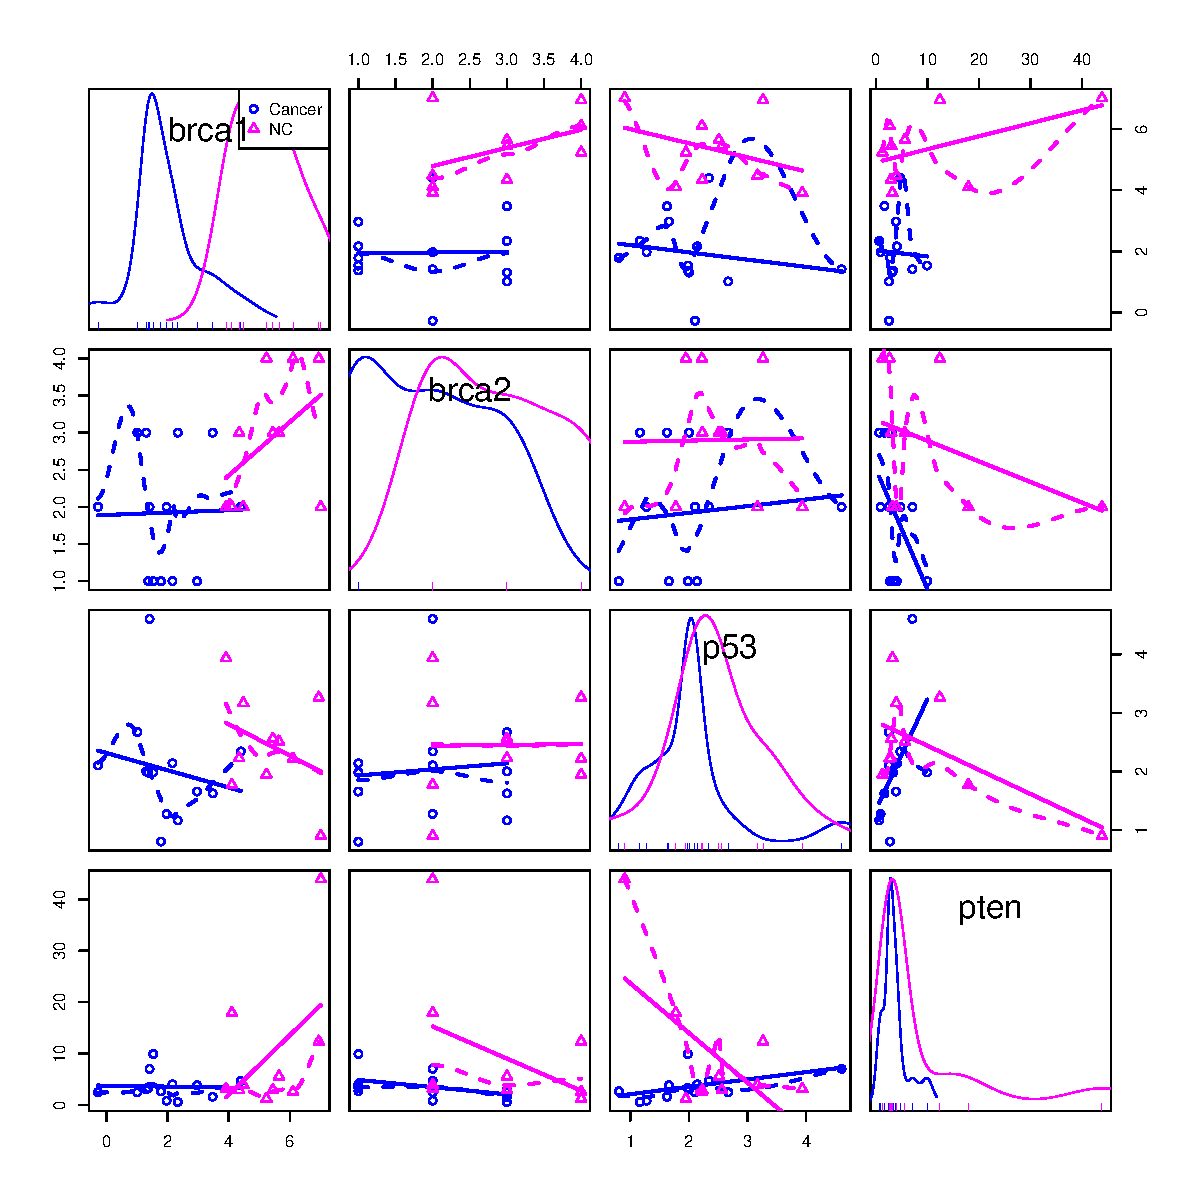
\includegraphics[width=\maxwidth]{figure/unnamed-chunk-132-1} 
\end{knitrout}

No vamos a seguir con esto. Pero se puede y probablemente desee mirar a este tipo de gráficos de forma rutinaria.

\section{Comparar dos grupos con t-test}
La forma más sencilla de realizar un test de la t es mediante:
\begin{knitrout}
\definecolor{shadecolor}{rgb}{0.969, 0.969, 0.969}\color{fgcolor}\begin{kframe}
\begin{alltt}
\hlkwd{t.test}\hldef{(p53} \hlopt{~} \hldef{cond,} \hlkwc{data} \hldef{= dp53)}
\end{alltt}
\begin{verbatim}
## 
## 	Welch Two Sample t-test
## 
## data:  p53 by cond
## t = -1.1376, df = 20.206, p-value = 0.2686
## alternative hypothesis: true difference in means between group Cancer and group NC is not equal to 0
## 95 percent confidence interval:
##  -1.2018502  0.3532041
## sample estimates:
## mean in group Cancer     mean in group NC 
##             2.028077             2.452400
\end{verbatim}
\end{kframe}
\end{knitrout}

La prueba t estándar asume que las varianzas de los dos grupos son iguales, mientras que la prueba de Welch no requiere que las varianzas de ambos grupos sean iguales. En la prueba de Welch, los grados de libertad pueden ser un número no entero (como sucede en este caso: \textit{df = 17.402}). Con este estadístico, el programa ha utilizado la distribución t correspondiente y ha calculado el área en ambas colas de la distribución.

\subsection{Grados de libertad}
Supongamos que tenemos los números 0, 1 y 2, y sabemos que su media es 1. Dado que tenemos tres números, ¿a cuántos de ellos podemos asignar libremente un valor? A dos de ellos, ya que el tercer número debe ajustarse para que el promedio sea 1. Así, el número de grados de libertad es el número de observaciones menos el número de parámetros que debemos estimar. En el caso de tener dos grupos, los grados de libertad se calcularían como:
$$ N = N_1 + N_2 = N - 2$$
o de manera equivalente:
$$(N_1 - 1) + (N_2 - 1) = N - 2$$

\subsection{Test de Welch vs test de la t}
Si las varianzas no son iguales y se realiza una prueba t estándar asumiendo que son iguales, se incurre en un error. En cambio, si las varianzas son realmente iguales, pero se usa la prueba de Welch, el error cometido es menor. Por ello, es preferible utilizar la prueba de Welch cuando existe incertidumbre sobre la igualdad de varianzas. Esta es la razón por la cual, por defecto, se suele optar por la prueba de Welch.


El test de la t sirve para \textbf{comparar medias}. La fórmula es:
\[
t = \frac{(\bar{x_1} - \bar{x_2})-(\mu_1 - \mu_2)}{S_{\bar{x_1}-\bar{x_2}}}
\]

\subsection{Desviación estándar vs error estándar}
La desviación estándar es una medida de la dispersión de los datos alrededor de la media, mostrando cuán alejados están los valores individuales del promedio. Es útil para entender la variabilidad dentro de una sola muestra o población. La desviación (\sigma: poblacional; s: muestral) disminuye cuadráticamente con el tamaño poblacional o muestral, respectivamente:
\[
\sigma^2 = \frac{1}{N} \sum_{i=1}^{N} (x_i - \mu)^2      s^2 = \frac{1}{n - 1} \sum_{i=1}^{n} (x_i - \bar{x})^2
\]
En cambio, el error estándar mide la precisión de la media muestral como estimador de la media poblacional. A diferencia de la desviación estándar, que refleja la variabilidad en una muestra específica, el error estándar indica cuánto podrían variar las medias de diferentes muestras si se extrajeran repetidamente de la misma población. Cuanto mayor es el tamaño de la muestra, menor será el error estándar, ya que la media muestral se aproxima más a la media poblacional.
$$ E[\bar{X}] = \mu ;      E[S^2] \neq \sigma^2$$

\subsection{Ideas clave sobre el test de la t}
Es importante comprender algunas ideas clave sobre el uso de los p-valores en la prueba de hipótesis. Primero, cuando el resultado de un análisis no es estadísticamente significativo, no estamos confirmando la hipótesis nula; simplemente es posible que estemos fallando en rechazarla, lo que significa que no hemos encontrado suficiente evidencia en su contra. Además, el p-valor no representa la probabilidad de que la hipótesis nula sea cierta, ni de que la hipótesis alternativa lo sea. En cambio, el p-valor sirve como una métrica que indica la fuerza de la evidencia \textbf{en contra} de la hipótesis nula. Si el p-valor es bajo, la interpretación es que, \textit{"o bien la hipótesis nula es falsa, o bien hemos observado un evento tan (\textbf{im})probable como el p-valor calculado, dado que la hipótesis nula es cierta"}.

Estas tres preguntas son distintas: 
1) ¿Qué dice la evidencia? Esto lo responde el p-valor. <-- prueba estadística
2) ¿Qué debo creer? Quizás hay evidencia adicional. <-- inferencia bayesiana
3) ¿Qué debo hacer? Esto refleja otra relación de coste-beneficio. <-- T.^{a} de la decisión

Es fundamental recordar que los p-valores se calculan bajo ciertos supuestos de modelo, y cualquier violación de estos supuestos puede afectar la validez del resultado. Por eso, utilizar los p-valores de manera cuidadosa es más adecuado que interpretar resultados en términos absolutos de “significativo” o “no significativo”. Además, comparar valores extremadamente pequeños de p (como $p = 10^{-13}$ frente a $p = 10^{-16}$) no tiene un significado práctico adicional, ya que ambos ya representan un nivel de evidencia considerablemente fuerte en contra de la hipótesis nula. También es esencial reconocer que el p-valor no es la única herramienta de inferencia estadística; los intervalos de confianza proporcionan información valiosa sobre el rango de valores plausibles para el parámetro de interés, complementando el análisis de los p-valores y ayudando a interpretar mejor los resultados.

Para comprender la inferencia estadística, es esencial distinguir entre una muestra y la población. La población es el conjunto completo de elementos sobre el cual queremos obtener conclusiones, mientras que una muestra es un subconjunto de esa población que se selecciona para su análisis. Mayoritariamente, se trabaja con muestras porque estudiar toda una población suele ser impracticable; a partir de los datos de la muestra, hacemos inferencias sobre las características de la población.

Un concepto fundamental en estadística es el de un estadístico, que es cualquier valor numérico que se puede calcular a partir de una muestra. Un tipo específico de estadístico es un estimador, que se usa para aproximar un parámetro de la población. Por ejemplo, la media muestral, calculada como $\sum x/N$, es un estimador que proporciona una aproximación de la media poblacional verdadera utilizando datos de una muestra.

Un tipo particular de estadístico es el estadístico t, utilizado en la prueba t para contrastar hipótesis sobre las medias de dos grupos. Tanto los estadísticos en general como los estimadores específicos tienen distribuciones propias, que describen cómo se distribuyen sus valores posibles si el muestreo se repitiera muchas veces. Esta variabilidad introducida por el muestreo afecta las conclusiones y debe tenerse en cuenta.

Otro aspecto clave es entender la diferencia entre desviación estándar y error estándar. La desviación estándar mide la variabilidad de los datos dentro de la muestra, mientras que el error estándar refleja la variabilidad de la media muestral con respecto a la media poblacional.

En cuanto al p-valor, es una medida de la evidencia en contra de la hipótesis nula (H0), que plantea que no hay efecto o diferencia. Al calcular el p-valor, se supone que los estadísticos siguen una distribución específica bajo la hipótesis nula, lo cual permite evaluar la probabilidad de obtener un resultado tan extremo como el observado.

La lógica de un test estadístico radica en decidir entre la hipótesis nula y la alternativa basándose en los datos. A diferencia de un procedimiento de estimación, que busca obtener un valor aproximado de un parámetro, una prueba de hipótesis se centra en determinar si la evidencia es suficientemente fuerte para rechazar la hipótesis nula. Esta diferencia entre estimación y prueba de hipótesis es fundamental para realizar inferencias estadísticas bien informadas.

\subsection{Intervalos de confianza}
Un intervalo de confianza del 95\% alrededor de una estimación, como una media, no debe interpretarse como que existe una probabilidad del 95\% de que la media poblacional esté entre los límites del intervalo, por ejemplo, entre 1 y 2. Esta interpretación es incorrecta. La interpretación correcta de un intervalo de confianza del 95\% es que, si repitiéramos el muestreo y el cálculo del intervalo de confianza muchas veces, aproximadamente el 95\% de esos intervalos generados contendrían la media poblacional real. El intervalo refleja la precisión de la estimación dada la variabilidad del muestreo, no una probabilidad sobre la ubicación de la media en un intervalo específico para una muestra concreta.

En el contexto de un test de hipótesis, si el test es justamente significativo (es decir, si el p-valor es 0,05), uno de los límites del intervalo de confianza tocará el valor de 0, indicando que no se puede rechazar la hipótesis nula con un nivel de confianza superior al 95\%. Cuando el valor t calculado aumenta (es decir, la evidencia contra la hipótesis nula se vuelve más fuerte), el intervalo de confianza se amplía, reflejando una mayor certeza en la estimación. Por ejemplo, un valor t de 18 corresponde a un área bajo la curva mucho mayor que un valor t de 4, lo que implica una estimación mucho más precisa y una evidencia más fuerte en favor de rechazar la hipótesis nula.

\subsection{Supuestos del test de la t}
Un supuesto clave en la prueba t es la \textbf{independencia de los datos}. Este requisito no solo es esencial para la prueba t, sino también para muchas otras pruebas estadísticas. La falta de independencia entre observaciones es un problema grave y común en los estudios estadísticos. Una forma de dependencia, conocida como pseudorreplicación, ocurre cuando las observaciones no son realmente independientes, lo que puede sesgar los resultados y llevar a interpretaciones incorrectas.

Cuando se comparan dos medias, otro supuesto importante es la \textbf{igualdad de varianzas}. Sin embargo, detectar diferencias en las varianzas no siempre es sencillo. Dos soluciones prácticas ante la posible desigualdad de varianzas son el uso de la prueba de Welch (predeterminada en software estadístico como R) y la aplicación de transformaciones de datos. No obstante, antes de continuar con la comparación, conviene preguntarse si realmente tiene sentido comparar medias cuando las varianzas de los grupos difieren considerablemente, ya que diferencias amplias en la variabilidad pueden afectar la interpretación de las medias.

En cuanto a la \textbf{normalidad} de los datos, este supuesto es menos restrictivo, especialmente a medida que aumenta el tamaño de la muestra. Es importante notar que, al hablar de normalidad, simetría y otros aspectos de la distribución, se hace referencia a la \textbf{distribución de cada grupo por separado}. Las desviaciones de la normalidad debido a la \textit{asimetría} pueden tener un efecto significativo en los resultados, mientras que las desviaciones relacionadas con una mayor o menor \textit{curtosis} (colas más pesadas o ligeras que la normal) suelen tener un impacto menor. Por eso, comúnmente se acepta que los datos estén "suficientemente cerca de la normalidad," prestando especial atención a la asimetría de la distribución. Con tamaños de muestra grandes, la normalidad de los datos suele ser menos preocupante gracias al \textit{teorema del límite central}, que establece que, a medida que aumenta el tamaño de la muestra, la distribución de la media muestral se aproxima a una distribución normal. ¿Cuándo una muestra es lo suficientemente grande? La respuesta depende de cuánto difieran los datos de la normalidad. En muchas situaciones, un tamaño de muestra de 10 puede ser suficiente; 50 generalmente es adecuado y, en algunos casos, incluso muestras de 100 observaciones podrían no ser suficientes si la distribución es extremadamente no normal.

Por último, los \textbf{valores atípicos o outliers} pueden ser una preocupación seria en el análisis de datos. De hecho, los valores atípicos, o los valores potencialmente atípicos según alguna definición, son identificados por la función \code{Boxplots} en R. En general, los puntos que están muy alejados del resto de los datos pueden tener efectos graves sobre la media calculada, pero no sobre la mediana (esto es uno de los motivos por los cuales los procedimientos no paramétricos suelen ser más robustos frente a valores atípicos). Sin embargo, decidir qué hacer con los valores atípicos no es una tarea sencilla. Un valor atípico podría ser el resultado de un error en el registro de los datos, pero también podría ser un dato perfectamente válido y, de hecho, podría ser lo “interesante” del análisis. En algunos casos, se realizan análisis con y sin el valor atípico para comparar los resultados (y, por supuesto, se debe informar explícitamente de esto). A veces, se llegan a las mismas conclusiones cualitativas, pero otras veces no. Por tanto, antes de decidir cómo tratar los valores atípicos, es fundamental reflexionar cuidadosamente sobre lo que se considera un valor atípico en el contexto del análisis y el objetivo del estudio. No se debe caer en la tentación de eliminar automáticamente los valores atípicos sin una justificación sólida. Y, en cualquier caso, cualquier decisión sobre cómo tratar los valores atípicos debe ser documentada y comunicada de manera transparente.

%13/11 - Ramón
\section{Tests de una y dos colas}
Hasta ahora, hemos trabajado con tests de dos colas. Sin embargo, en algunas situaciones es posible limitar el análisis a una sola cola. En un test de dos colas, la hipótesis nula plantea que las medias son iguales, y cualquier desviación en ambas direcciones puede llevar al rechazo de la hipótesis nula. En contraste, un test de una cola permite especificar una dirección para la hipótesis. Por ejemplo, podemos plantear como hipótesis nula que $\mu_1 \geq \mu_2$, y como hipótesis alternativa que $\mu_1 < \mu_2$, concentrándonos solo en una dirección de la desviación.

Para un mismo estadístico t, un test de una cola tendrá un p-valor igual a la mitad del p-valor de un test de dos colas, ya que se considera únicamente una de las colas de la distribución. Sin embargo, por convención y para evitar sesgos, lo normal es realizar un test de dos colas, especialmente si no existe una razón científica sólida para anticipar la dirección del efecto.

Algunos tests, como el ANOVA, utilizan la distribución F, la cual tiene una sola cola de manera natural, ya que evalúa si existe variabilidad significativa entre varios grupos en cualquier dirección sin considerar una dirección específica. En el caso del test de la t, se debe decidir entre un test de una o dos colas en función de la hipótesis científica planteada y siempre antes de observar los datos, para evitar que los resultados influyan en la elección del tipo de test.

\section{Potencia de un test}
Si existe una verdadera diferencia de medias, nos gustaría detectarla. La potencia se refiere a nuestra capacidad para rechazar el nulo cuando es falso. Esta figura puede ayudar; las filas se refieren al estado real del Universo y las columnas a la decisión que se toma.

\begin{table}[h!]
\begin{tabular}{p{6.5cm}|>{\centering}p{2.5cm}|>{\centering}p{2.5cm}|}
  \multicolumn{1}{c}{} & \multicolumn{1}{>{\centering}p{2.5cm}}{Hipótesis nula no se rechaza} &
  \multicolumn{1}{>{\centering}p{2.5cm}}{Hipótesis nula se rechaza}\tabularnewline
  \cline{2-3}
  Medias no difieren ($H_0$ \textit{es cierta}) & Correcto & Type I error\tabularnewline
  \cline{2-3}
  Medias difieren ($H_0$ \textit{es falsa}) & Type II error & Correcto\tabularnewline
  \cline{2-3}
\end{tabular}
\end{table}

No es posible realizar un test con un error de tipo I extremadamente pequeño sin aumentar el error de tipo II, ya que reducir al mínimo la probabilidad de un error de tipo I generalmente incrementa la probabilidad de un error de tipo II. Por ello, es necesario encontrar un equilibrio adecuado entre ambos tipos de error. Al diseñar un test, se debe establecer un nivel de significancia o error de tipo I nominal, generalmente expresado como $\alpha$, que refleje la probabilidad aceptable de rechazar la hipótesis nula cuando en realidad es cierta. Este valor nominal permite controlar de forma explícita la tasa de error de tipo I, manteniendo el test en un nivel de confianza apropiado para los objetivos del estudio.

La potencia es $1 - Type\ II\ error$. La potencia es la probabilidad de rechazar la hipótesis nula cuando la hipótesis nula es falsa.

La probabilidad de que se detecte una diferencia que realmente existe (potencia) depende de:
\begin{itemize}
\item El umbral que se utilice para decir que "las medias difieren" ($\alpha$ o error de tipo I).\footnote{El valor p es una función de los datos, es algo que se calcula con un procedimiento determinado para un conjunto de datos determinado; el nivel $\alpha$ o la tasa de error de tipo I es una propiedad del procedimiento.}
\item El tamaño de la muestra
\item El tamaño del efecto (distancia de medias)
\item La desviación estándar de la población
\end{itemize}

La potencia se puede calcular de antemano para saber si es probable encontrar una diferencia en caso de que la haya (dado el tamaño de la muestra y los tamaños de efecto y las desviaciones estándar estimados) y averiguar si el tamaño de la muestra es adecuado para la potencia deseada (y los tamaños del efecto y las desviaciones estándar estimados). Es importante recalcar que no tiene mucho sentido calcular la potencia del test después de haberlo calculado, ya que no aporta nada de valor.

\subsection{Maldición del ganador}
%Cuando se hacen estudios con poca potencia estadística, los efectos que se detectan, es decir, aquellas comparaciones que superan el punto de corte (p valor inferior a 0,05) suelen ser comparaciones asociadas con una sobreestimación del verdadero efecto. 
En estudios con baja potencia, las estimaciones de los efectos de las pruebas que resultan "significativas" tienden a estar sesgadas al alza, es decir, a ser mayores de lo que realmente deberían ser. Esto significa que, para un mismo fenómeno, cuando solo se consideran estudios de baja potencia con valores p significativos, las estimaciones del efecto suelen ser excesivamente grandes (en términos absolutos). Así, el sesgo de publicación, junto con la baja potencia, puede llevar a una sobreestimación sistemática de los tamaños del efecto reportados en la literatura.

Además, el tamaño de la muestra afecta el valor de p asociado a un estadístico t dado. Para un mismo valor de t, un tamaño de muestra grande se traduce en un p-valor más pequeño que el que obtendríamos con un tamaño de muestra pequeño, lo que significa que la significancia estadística es más fácil de alcanzar con muestras grandes, incluso si el efecto real es pequeño. Este fenómeno subraya la importancia de interpretar los valores p en contexto, considerando tanto el tamaño de muestra como la potencia del estudio para obtener una estimación realista del efecto.

\section{(Bio)equivalencia}
Hemos configurado las cosas de modo que \textbf{necesitamos pruebas suficientemente sólidas para rechazar el nulo} y \textbf{utilizamos p-valores de medidas de fuerza de las pruebas CONTRA el nulo}. Esto es a menudo lo que queremos en la ciencia, pero no siempre. Y en muchos casos, en particular en cuestiones relacionadas con la salud pública, es posible que queramos seguir un principio de precaución.

Por ejemplo, tal vez queramos decir: «Sólo permitiremos verter cloro en el río si hay pruebas suficientemente sólidas de que tal acción no causará daños, por ejemplo, no aumentará la mortalidad de los peces». Esto no es algo que se pueda resolver con valores p tal y como los hemos utilizado. 

¿Qué podemos hacer? Queremos darle la vuelta al proceso. Querríamos un procedimiento para responder a la siguiente pregunta: «¿Existen pruebas suficientemente sólidas de que, si el cloro tiene un efecto, éste no es mayor que un aumento de la mortalidad de los peces del 1\%?». Esto es como invertir la carga de la prueba: es como si ahora quisiéramos pruebas a favor de una hipótesis que dice que las cosas no difieren en más de un valor dado, pequeño (es decir, parece que ahora queremos pruebas a favor de lo que a menudo es el nulo). En otras palabras, queremos pruebas sólidas de que el valor verdadero está dentro de los límites de equivalencia, los límites que dicen que «las cosas son similares o equivalentes» (hemos simplificado las cosas aquí, preocupándonos sólo por los aumentos en la mortalidad de los peces, pero a menudo nos preocupamos por las desviaciones tanto hacia arriba como hacia abajo).

Podemos enfocar este problema como la búsqueda de pruebas contra la hipótesis (nueva nula) de que las cosas difieren en más de la tolerancia especificada, en nuestro caso ese 1\% de aumento en la mortalidad de los peces; en otras palabras, que el valor verdadero cae fuera de los límites de equivalencia. Si podemos rechazar nuestra nueva hipótesis nula de que los grupos difieren en más de un umbral determinado (que la diferencia real queda fuera de los límites de equivalencia), habremos establecido que son equivalentes. En algunos casos es relativamente sencillo hacerlo (como con el procedimiento TOST; realizando dos tests de una cola), pero en muchos otros no lo es.

\section{Inferencia bayesiana}
El teorema de Bayes es una fórmula fundamental en probabilidad condicional que permite calcular la probabilidad de un evento dado que otro evento ha ocurrido. Su expresión general es:
$$P(A|B) = \frac{P(B|A) \cdot P(A)}{P(B)}$$

En estadística, el teorema de Bayes se aplica de la siguiente manera:
$$P(H_0|\bar{x_A}-\bar{x_B} = 3) = \frac{P(\bar{x_A}-\bar{x_B} = 3 | H_0) \cdot P(H_0)}{P(\bar{x_A}-\bar{x_B} = 3)}$$

Sin embargo, una dificultad importante en la aplicación de la inferencia bayesiana en este contexto es la estimación de la probabilidad previa de la hipótesis nula, $P(H_0)$, antes de realizar el test. Asignar un valor adecuado a esta probabilidad previa es crucial, pero puede ser complicado y, en algunos casos, controvertido.

El teorema de Bayes es ampliamente utilizado en estadística sin controversias en áreas como el diagnóstico médico. Por ejemplo, calcular la probabilidad de padecer una enfermedad dado un resultado positivo en un test diagnóstico es una aplicación común. 
Sin embargo, la interpretación de un mismo resultado depende del contexto que se tenga.
En el caso de un test de sangre en heces para detectar cáncer de colon, un resultado positivo no necesariamente implica que la persona tenga la enfermedad, debido a la posibilidad de falsos positivos. En estos casos, el teorema de Bayes nos ayuda a comprender la probabilidad real de la enfermedad, considerando tanto la precisión del test como la prevalencia de la enfermedad en la población.

\section{Intervalos de confianza e interpretación de p-valores}
Al interpretar intervalos de confianza, es crucial considerar tanto la posición de la media como el rango en el que se concentra la mayor parte de los valores posibles.

Supongamos los siguientes intervalos de confianza en los que la hipótesis nula es $H_0 = \mu_1 - \mu_2 = 0$.

En el caso del primer intervalo de confianza, aunque incluye el valor 0 y, por tanto, no se rechaza la hipótesis nula, la media estimada está bastante alejada de 0, lo que sugiere que muchos de los valores dentro del intervalo no son consistentes con la hipótesis nula. Esto podría ser indicativo de un tamaño de muestra pequeño, y no rechazar la hipótesis nula sin más podría no ser adecuado. En el segundo caso, la hipótesis nula se rechaza, y el intervalo de confianza, que es pequeño y distante de 0, respalda una diferencia clara. Sin embargo, si el intervalo estuviera cerca de 0, rechazar la hipótesis nula podría tener menos relevancia práctica, ya que los valores observados indicarían una diferencia mínima.

Es importante recordar que los intervalos de confianza del 99\% son más amplios que los del 95\%, y estos, a su vez, son más amplios que los del 90\%. Cuanto mayor es el nivel de confianza, más amplio será el intervalo, lo que refleja una mayor incertidumbre en la estimación.

Hay que evitar conclusiones erróneas al interpretar significación estadística. No siempre es contradictorio que un estudio resulte "significativo" mientras otro no lo sea, incluso si el efecto observado es el mismo en ambos. Por ejemplo, un estudio con un p-valor bajo (significativo) y otro con un p-valor alto (no significativo) pueden tener medias similares si el tamaño de muestra o la variabilidad difieren entre los estudios.

\begin{figure}[h!]
\centering
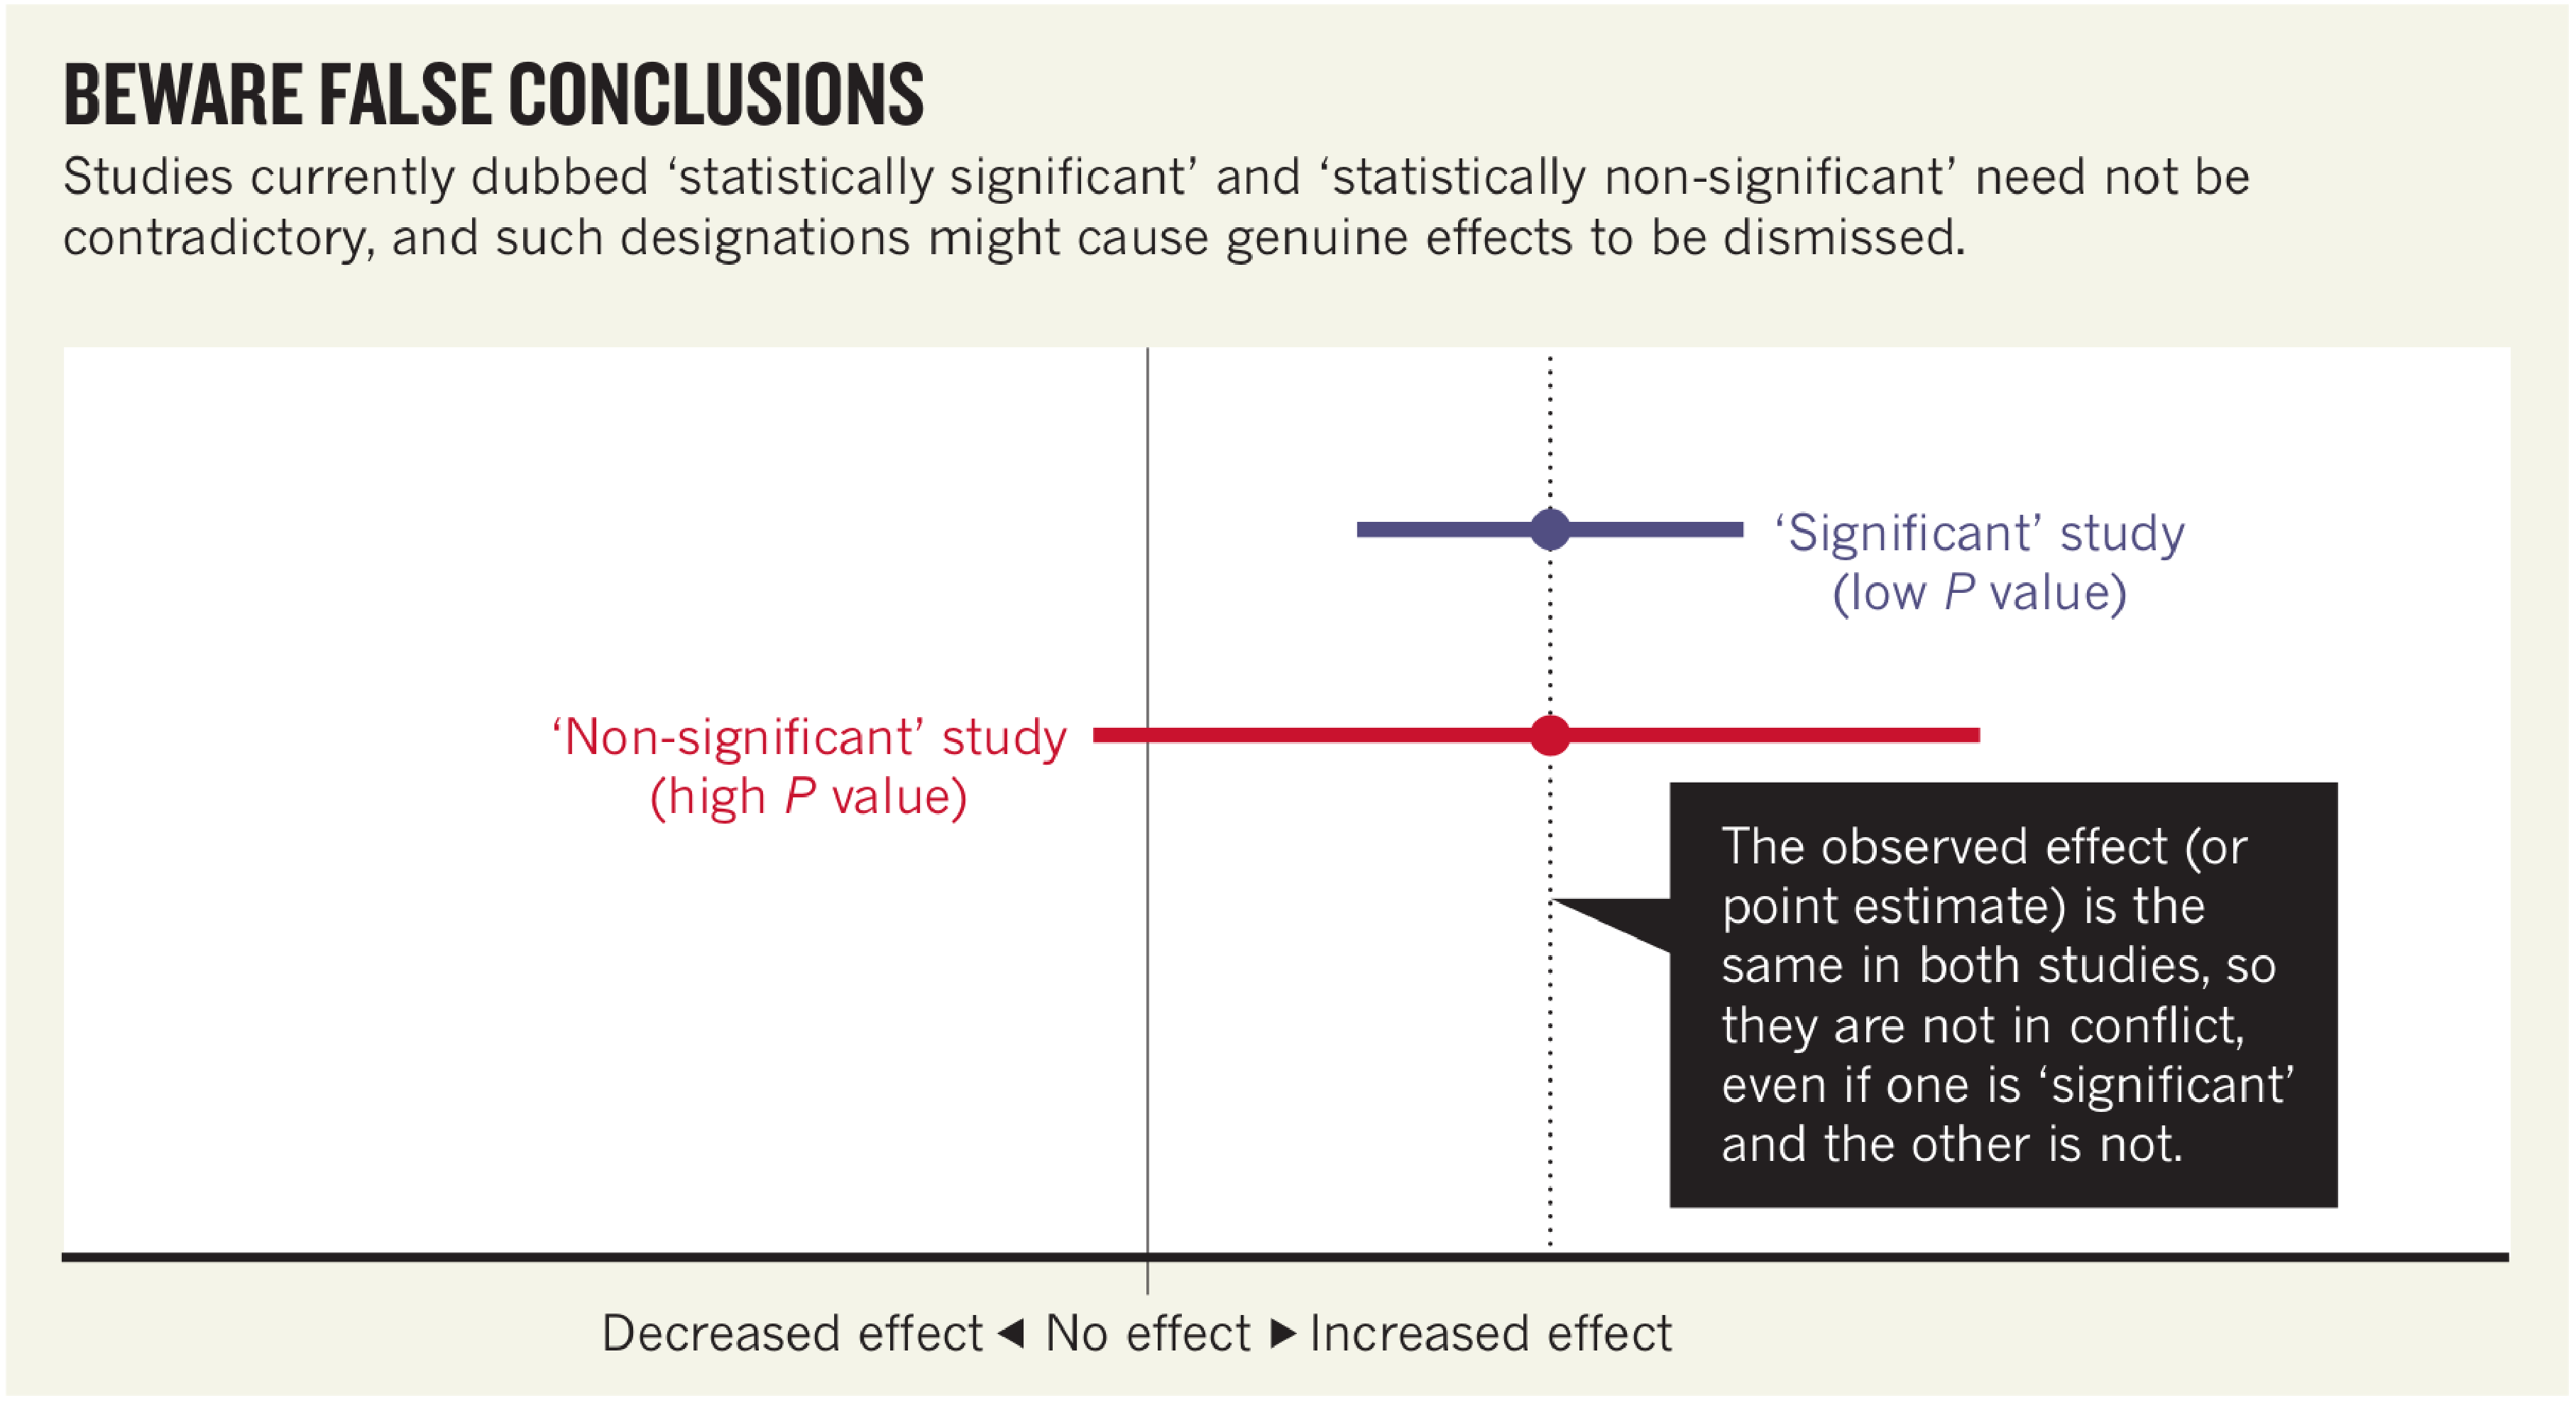
\includegraphics[width = 0.9\textwidth]{figs/amrhein.pdf}
\end{figure}

Los intervalos de confianza, en general, ofrecen más información que los p-valores, ya que muestran los valores que son consistentes con lo observado y permiten evaluar el rango de posibles efectos. En el gráfico, ambos intervalos muestran valores compatibles con la hipótesis alternativa, sugiriendo una diferencia entre grupos.

Finalmente, la interpretación de un p-valor adecuado depende del contexto. Aunque históricamente se ha utilizado un umbral de 0,05, en ciertos contextos este nivel puede ser demasiado alto, y puede ser necesario establecer un criterio más estricto o considerar otras métricas adicionales según la naturaleza del estudio.

\section{Tests apareados}
Los tests apareados son un tipo de análisis estadístico diseñado para comparar dos medidas tomadas sobre el mismo grupo de individuos o unidades experimentales bajo condiciones distintas. Su uso es especialmente común en estudios donde se desea evaluar el efecto de un tratamiento o intervención midiendo a los mismos sujetos en dos momentos diferentes (pre y post intervención) o bajo dos condiciones diferentes. Al comparar cada sujeto consigo mismo, estos tests ayudan a controlar la variabilidad intrasujeto y, por tanto, pueden aumentar la precisión y potencia estadística en comparación con un test de muestras independientes.

En los tests apareados, el análisis se enfoca en las diferencias intrasujeto (o intraunidad), lo que permite aislar el efecto de la condición o el tiempo sobre cada individuo. El test de la t apareado, una de las pruebas más usadas para este tipo de análisis, evalúa si la media de las diferencias entre dos medidas es significativamente distinta de cero, lo cual indicaría una diferencia sistemática entre las condiciones evaluadas.

Para que los resultados de un test apareado sean válidos, es crucial que las medidas sean independientes entre sujetos y que cada par de medidas esté correctamente ordenado para cada sujeto. Esto asegura que cada par se refiera al mismo individuo en ambas condiciones, de manera que el test pueda evaluar directamente las diferencias intrasujeto.

\begin{knitrout}
\definecolor{shadecolor}{rgb}{0.969, 0.969, 0.969}\color{fgcolor}\begin{kframe}
\begin{alltt}
\hlkwd{set.seed}\hldef{(}\hlnum{15}\hldef{)}
\hldef{s} \hlkwb{<-} \hlkwd{rnorm}\hldef{(}\hlnum{12}\hldef{,} \hlnum{4}\hldef{,} \hlnum{25}\hldef{)}

\hldef{s} \hlkwb{<-} \hlkwd{c}\hldef{(s, s)}
\hldef{cond} \hlkwb{<-} \hlkwd{rep}\hldef{(}\hlkwd{c}\hldef{(}\hlnum{0}\hldef{,} \hlnum{.5}\hldef{),} \hlkwd{c}\hldef{(}\hlnum{12}\hldef{,} \hlnum{12}\hldef{))}
\hldef{y} \hlkwb{<-} \hlkwd{rnorm}\hldef{(}\hlnum{24}\hldef{)} \hlopt{+} \hldef{s} \hlopt{+} \hldef{cond}
\hldef{y} \hlkwb{<-} \hldef{y} \hlopt{-} \hlkwd{min}\hldef{(y)} \hlopt{+} \hlnum{0.3}
\hldef{id} \hlkwb{<-} \hlkwd{replicate}\hldef{(}\hlnum{12}\hldef{,} \hlkwd{paste}\hldef{(}\hlkwd{sample}\hldef{(letters,} \hlnum{10}\hldef{),} \hlkwc{collapse} \hldef{=} \hlsng{""}\hldef{))}
\hldef{id} \hlkwb{<-} \hlkwd{c}\hldef{(id, id)}
\hldef{dmyc} \hlkwb{<-} \hlkwd{data.frame}\hldef{(}\hlkwc{myc} \hldef{=} \hlkwd{round}\hldef{(y,} \hlnum{3}\hldef{),}
                   \hlkwc{cond} \hldef{=} \hlkwd{rep}\hldef{(}\hlkwd{c}\hldef{(}\hlsng{"Cancer"}\hldef{,} \hlsng{"NC"}\hldef{),} \hlkwd{c}\hldef{(}\hlnum{12}\hldef{,} \hlnum{12}\hldef{)),}
                   \hlkwc{id} \hldef{= id)}
\end{alltt}
\end{kframe}
\end{knitrout}

\subsection{Test de la t apareados}
\begin{knitrout}
\definecolor{shadecolor}{rgb}{0.969, 0.969, 0.969}\color{fgcolor}\begin{kframe}
\begin{alltt}
\hldef{myc.cancer} \hlkwb{<-} \hldef{dmyc}\hlopt{$}\hldef{myc[dmyc}\hlopt{$}\hldef{cond} \hlopt{==} \hlsng{"Cancer"}\hldef{]}
\hldef{myc.nc} \hlkwb{<-} \hldef{dmyc}\hlopt{$}\hldef{myc[dmyc}\hlopt{$}\hldef{cond} \hlopt{==} \hlsng{"NC"}\hldef{]}
\hlkwd{t.test}\hldef{(myc.nc, myc.cancer,} \hlkwc{paired} \hldef{=} \hlnum{TRUE}\hldef{)}
\end{alltt}
\begin{verbatim}
## 
## 	Paired t-test
## 
## data:  myc.nc and myc.cancer
## t = 4.079, df = 11, p-value = 0.001823
## alternative hypothesis: true mean difference is not equal to 0
## 95 percent confidence interval:
##  0.432056 1.444777
## sample estimates:
## mean difference 
##       0.9384167
\end{verbatim}
\end{kframe}
\end{knitrout}
En este análisis, se mide a 12 sujetos en dos condiciones diferentes, generando un total de 24 observaciones. Sin embargo, al tratarse de un test apareado, el análisis se enfoca en las 12 diferencias intrasujeto entre ambas condiciones, lo que implica que hay 11 grados de libertad.

El resultado del test de R muestra que se ha realizado un test apareado y proporciona el valor de t, los grados de libertad (df) y el p-valor asociado. Además, señala que la hipótesis alternativa es que la diferencia entre las medias de las dos condiciones no es igual a 0, refiriéndose a la diferencia intrasujeto.

El output incluye un intervalo de confianza del 95\% para la media de las diferencias, que en este caso está desplazado respecto al 0 (lo cual puede sugerir una diferencia significativa entre las condiciones). La media de las diferencias (\textit{mean differences}) indica el promedio de la variación intrasujeto entre ambas condiciones.

Es crucial que los datos estén correctamente ordenados para cada sujeto en ambas condiciones. Esto significa que los dos vectores pasados al test deben tener las observaciones de cada sujeto en el mismo orden, ya que el test apareado compara las diferencias exactas entre las condiciones para cada sujeto.

\subsection{Remodelación de los datos para un test emparejado}
Cuando se va a realizar un test de la t emparejado, se pueden organizar los datos en estructuras como las siguientes:

\begin{table}[h!]
\centering
\begin{tabular}{ccc}
  SubjectID&Tumor&Non-Tumor\\
  \hline
  pepe&23&45\\
  maria&29&56\\
  \ldots&\ldots&\ldots\\
\end{tabular}
\caption{Paired data in a ``unstacked or wide'' shape/format.}\label{unstacked}
\end{table}

\begin{table}[h!]
\centering
\begin{tabular}{ccc}
  SubjectID&Myc&Condition\\
  \hline
  pepe&23&tumor\\
  pepe&45&nontumor\\
  maria&29&tumor\\
  maria&56&nontumor\\
  \ldots&\ldots&\ldots\\
\end{tabular}
\caption{Paired data in a ``stacked or long'' shape/format.}\label{stacked}
\end{table}

En general, es más útil tener los datos organizada de forma "apilada".
\newpage
\begin{knitrout}
\definecolor{shadecolor}{rgb}{0.969, 0.969, 0.969}\color{fgcolor}\begin{kframe}
\begin{alltt}
\hldef{(merged3} \hlkwb{<-} \hlkwd{reshape}\hldef{(dmyc,} \hlkwc{direction} \hldef{=} \hlsng{"wide"}\hldef{,} \hlkwc{idvar} \hldef{=} \hlsng{"id"}\hldef{,}
                    \hlkwc{timevar} \hldef{=} \hlsng{"cond"}\hldef{,} \hlkwc{v.names} \hldef{=} \hlsng{"myc"}\hldef{))}
\end{alltt}
\begin{verbatim}
##            id myc.Cancer myc.NC
## 1  bqysitlvpm     38.289 39.634
## 2  zuhxmiyfos     76.188 78.361
## 3  bpkmxwhtsg     24.621 24.396
## 4  qsmyexkcnw     54.079 53.902
## 5  uhbkifsnvw     43.832 44.679
## 6  efzpcboidt      0.300  1.675
## 7  trsyacmejh     31.055 32.260
## 8  hyqjownkue     58.402 59.427
## 9  ejmkobsqrh     29.723 30.300
## 10 mculjayvhw      6.190  6.030
## 11 ytwgsplaef     52.626 54.494
## 12 dchlnopykg     22.089 23.497
\end{verbatim}
\begin{alltt}
\hldef{dmycWide} \hlkwb{<-} \hlkwd{reshapeL2W}\hldef{(dmyc,} \hlkwc{within}\hldef{=}\hlsng{"cond"}\hldef{,} \hlkwc{id}\hldef{=}\hlsng{"id"}\hldef{,} \hlkwc{varying}\hldef{=}\hlsng{"myc"}\hldef{)}
\end{alltt}
\end{kframe}
\end{knitrout}

\subsection{El test de la t emparejado - plots}
\begin{knitrout}
\definecolor{shadecolor}{rgb}{0.969, 0.969, 0.969}\color{fgcolor}\begin{kframe}
\begin{alltt}
\hlcom{## Paired}
\hlkwd{t.test}\hldef{(merged3}\hlopt{$}\hldef{myc.NC, merged3}\hlopt{$}\hldef{myc.Cancer,} \hlkwc{alternative}\hldef{=}\hlsng{'two.sided'}\hldef{,}
       \hlkwc{conf.level}\hldef{=}\hlnum{.95}\hldef{,}  \hlkwc{paired}\hldef{=}\hlnum{TRUE}\hldef{)}
\end{alltt}
\begin{verbatim}
## 
## 	Paired t-test
## 
## data:  merged3$myc.NC and merged3$myc.Cancer
## t = 4.079, df = 11, p-value = 0.001823
## alternative hypothesis: true mean difference is not equal to 0
## 95 percent confidence interval:
##  0.432056 1.444777
## sample estimates:
## mean difference 
##       0.9384167
\end{verbatim}
\end{kframe}
\end{knitrout}

\begin{knitrout}
\definecolor{shadecolor}{rgb}{0.969, 0.969, 0.969}\color{fgcolor}\begin{kframe}
\begin{alltt}
\hlkwd{t.test}\hldef{(myc} \hlopt{~} \hldef{cond,} \hlkwc{alternative} \hldef{=} \hlsng{'two.sided'}\hldef{,} \hlkwc{conf.level}\hldef{=}\hlnum{.95}\hldef{,}
       \hlkwc{var.equal}\hldef{=}\hlnum{FALSE}\hldef{,}  \hlkwc{data}\hldef{=dmyc)}
\end{alltt}
\begin{verbatim}
## 
## 	Welch Two Sample t-test
## 
## data:  myc by cond
## t = -0.10365, df = 21.996, p-value = 0.9184
## alternative hypothesis: true difference in means between group Cancer and group NC is not equal to 0
## 95 percent confidence interval:
##  -19.71435  17.83752
## sample estimates:
## mean in group Cancer     mean in group NC 
##             36.44950             37.38792
\end{verbatim}
\end{kframe}
\end{knitrout}

\begin{knitrout}
\definecolor{shadecolor}{rgb}{0.969, 0.969, 0.969}\color{fgcolor}\begin{kframe}
\begin{alltt}
\hlkwd{plotMeans}\hldef{(dmyc}\hlopt{$}\hldef{myc, dmyc}\hlopt{$}\hldef{cond,} \hlkwc{error.bars} \hldef{=} \hlsng{"se"}\hldef{,} \hlkwc{ylab} \hldef{=} \hlsng{"MYC"}\hldef{,}
          \hlkwc{xlab} \hldef{=} \hlsng{"Condition"}\hldef{)}
\end{alltt}
\end{kframe}
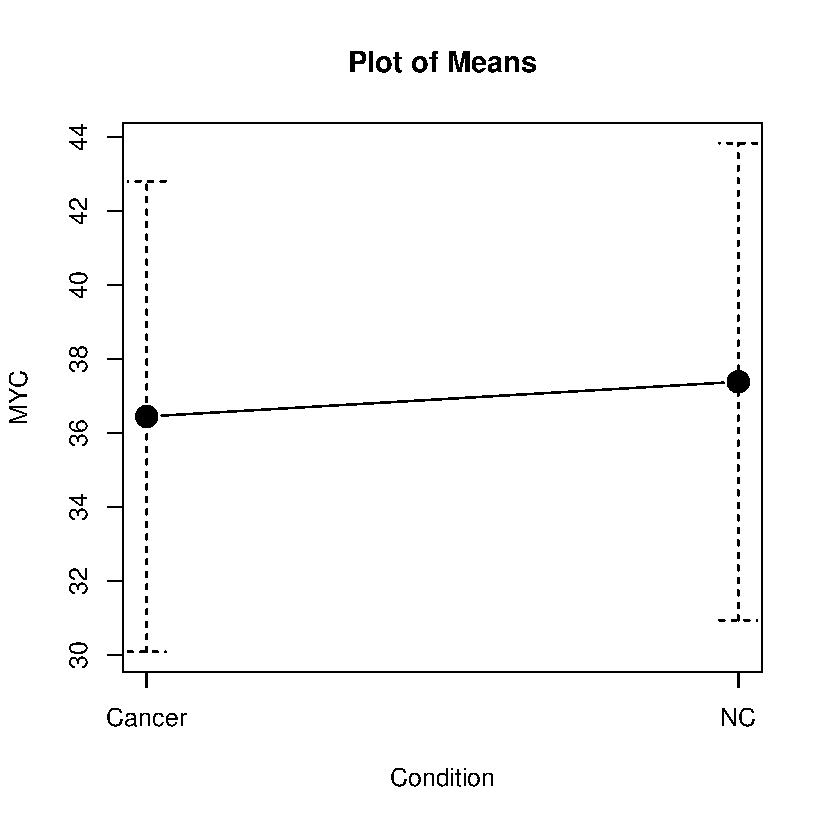
\includegraphics[width=\maxwidth]{figure/unnamed-chunk-138-1} 
\end{knitrout}

Los intervalos de confianza solapan a lo largo de sus recorridos. En general, es un mal plot para datos emparejados al no reflejarse que cada sujeto se ha medido en dos condiciones.

\begin{knitrout}
\definecolor{shadecolor}{rgb}{0.969, 0.969, 0.969}\color{fgcolor}\begin{kframe}
\begin{alltt}
\hldef{diff.nc.c} \hlkwb{<-} \hldef{(myc.nc} \hlopt{-} \hldef{myc.cancer)}
\hlkwd{t.test}\hldef{(diff.nc.c)}
\end{alltt}
\begin{verbatim}
## 
## 	One Sample t-test
## 
## data:  diff.nc.c
## t = 4.079, df = 11, p-value = 0.001823
## alternative hypothesis: true mean is not equal to 0
## 95 percent confidence interval:
##  0.432056 1.444777
## sample estimates:
## mean of x 
## 0.9384167
\end{verbatim}
\begin{alltt}
\hlkwd{Boxplot}\hldef{(} \hlopt{~} \hldef{diff.nc.c,} \hlkwc{data} \hldef{= merged3,} \hlkwc{xlab} \hldef{=} \hlsng{""}\hldef{,}
         \hlkwc{ylab} \hldef{=} \hlsng{"Intra-subject difference (NC - Cancer)"}\hldef{,} \hlkwc{main} \hldef{=} \hlsng{"MYC"}\hldef{)}
\end{alltt}
\end{kframe}
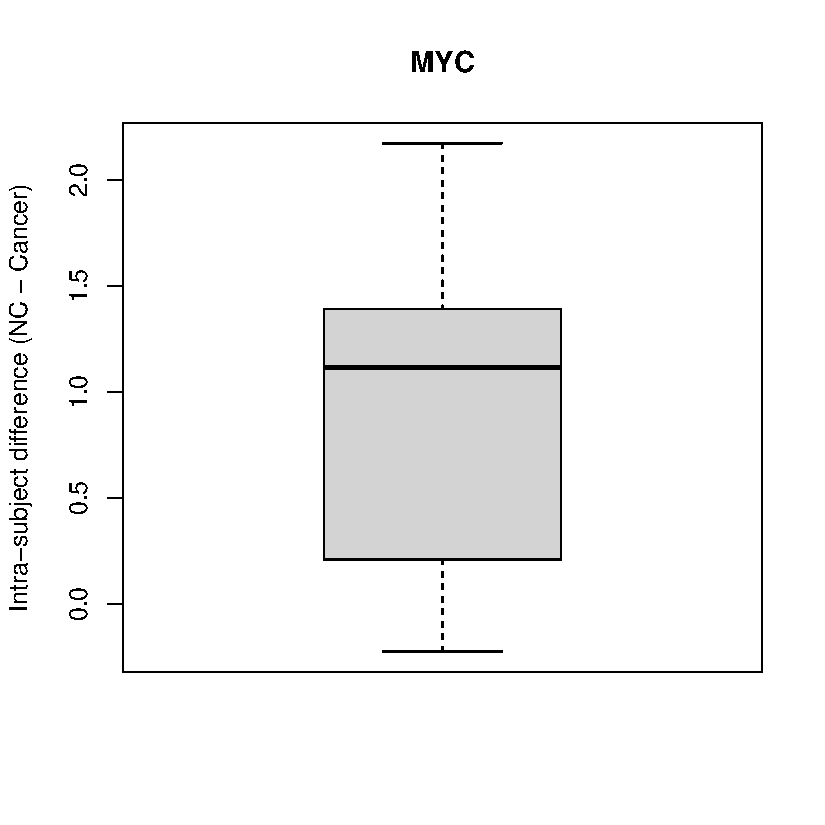
\includegraphics[width=\maxwidth]{figure/unnamed-chunk-139-1} 
\end{knitrout}
Aquí se calcula la diferencia intrasujeto y se muestra en el plot. Es una mejor representación, ya que el grueso de los pares son desviaciones positivas. 

\begin{knitrout}
\definecolor{shadecolor}{rgb}{0.969, 0.969, 0.969}\color{fgcolor}\begin{kframe}
\begin{alltt}
\hlkwd{library}\hldef{(ggplot2)}

\hldef{dftmp} \hlkwb{<-} \hlkwd{data.frame}\hldef{(}\hlkwc{y} \hldef{= dmycWide}\hlopt{$}\hldef{diff.nc.c)}
\hldef{theplot} \hlkwb{<-} \hlkwd{ggplot}\hldef{(}\hlkwc{data} \hldef{= dftmp,} \hlkwd{aes}\hldef{(}\hlkwc{x} \hldef{=} \hlkwd{factor}\hldef{(}\hlnum{1}\hldef{),} \hlkwc{y} \hldef{= y))} \hlopt{+}
  \hlkwd{geom_violin}\hldef{()} \hlopt{+} \hlkwd{geom_boxplot}\hldef{(}\hlkwc{width} \hldef{=} \hlnum{0.2}\hldef{)} \hlopt{+}
  \hlkwd{geom_jitter}\hldef{(}\hlkwc{colour} \hldef{=} \hlsng{"black"}\hldef{,} \hlkwc{width} \hldef{=} \hlnum{0.1}\hldef{,} \hlkwc{height} \hldef{=} \hlnum{0}\hldef{)} \hlopt{+}
  \hlkwd{scale_x_discrete}\hldef{(}\hlkwc{breaks} \hldef{=} \hlkwa{NULL}\hldef{)} \hlopt{+}
  \hlkwd{xlab}\hldef{(}\hlsng{""}\hldef{)} \hlopt{+}
  \hlkwd{ylab}\hldef{(}\hlsng{"Intra-subject difference (NC - Cancer)"}\hldef{)} \hlopt{+}
  \hlkwd{theme_bw}\hldef{(}\hlkwc{base_size} \hldef{=} \hlnum{14}\hldef{,} \hlkwc{base_family} \hldef{=} \hlsng{"sans"}\hldef{)} \hlopt{+}
  \hlkwd{theme}\hldef{(}\hlkwc{axis.title.x} \hldef{=} \hlkwd{element_blank}\hldef{(),} \hlkwc{axis.text.x} \hldef{=} \hlkwd{element_blank}\hldef{())}
\hlkwd{print}\hldef{(theplot)}
\hlkwd{rm}\hldef{(dftmp, theplot)}
\end{alltt}
\end{kframe}
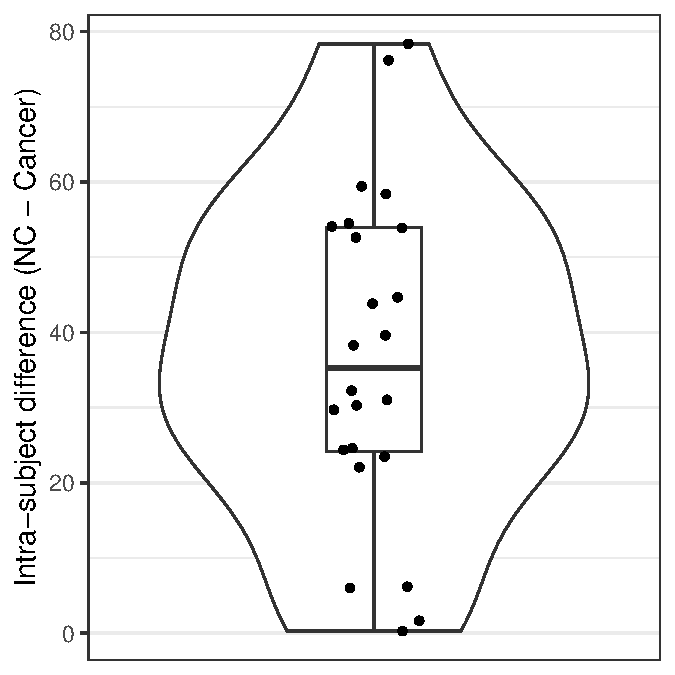
\includegraphics[width=\maxwidth]{figure/diff-violin-1} 
\end{knitrout}
Aquí, el número de observaciones es pequeño, por lo que el plot violín no está justificado; pero sería la mejor representación. Los puntos son las diferencias intrasujeto.

\begin{knitrout}
\definecolor{shadecolor}{rgb}{0.969, 0.969, 0.969}\color{fgcolor}\begin{kframe}
\begin{alltt}
\hlkwd{stripchart}\hldef{(myc} \hlopt{~} \hldef{cond,} \hlkwc{vertical} \hldef{=} \hlnum{TRUE}\hldef{,} \hlkwc{data} \hldef{= dmyc)}
\hlkwa{for}\hldef{(i} \hlkwa{in} \hlkwd{unique}\hldef{(dmyc}\hlopt{$}\hldef{id))}
  \hlkwd{segments}\hldef{(}\hlkwc{x0} \hldef{=} \hlnum{1}\hldef{,} \hlkwc{x1} \hldef{=} \hlnum{2}\hldef{,}
           \hlkwc{y0} \hldef{= dmyc}\hlopt{$}\hldef{myc[dmyc}\hlopt{$}\hldef{cond} \hlopt{==} \hlsng{"Cancer"} \hlopt{&} \hldef{dmyc}\hlopt{$}\hldef{id} \hlopt{==} \hldef{i],}
           \hlkwc{y1} \hldef{= dmyc}\hlopt{$}\hldef{myc[dmyc}\hlopt{$}\hldef{cond} \hlopt{==} \hlsng{"NC"} \hlopt{&} \hldef{dmyc}\hlopt{$}\hldef{id} \hlopt{==} \hldef{i],}
           \hlkwc{col} \hldef{=} \hlsng{"red"}\hldef{)}
\end{alltt}
\end{kframe}
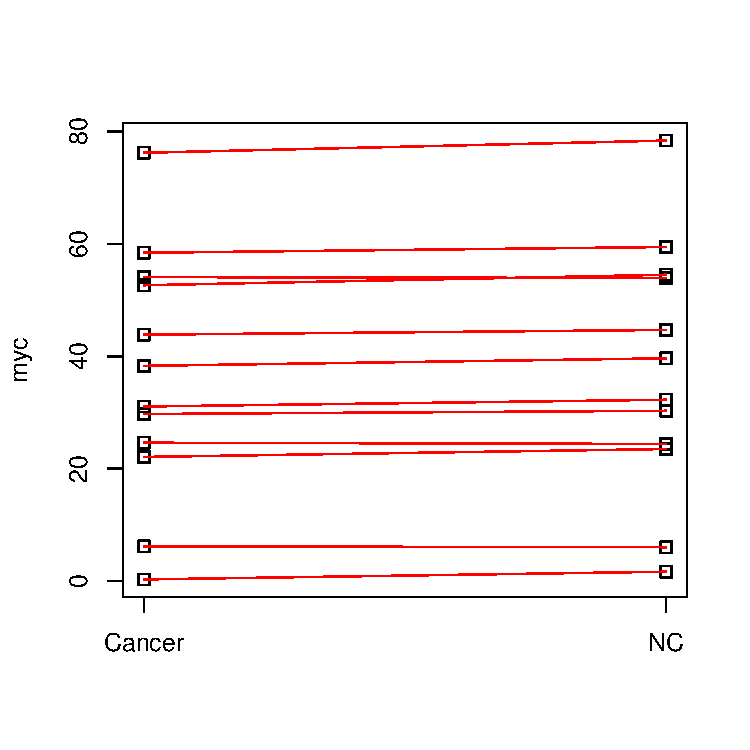
\includegraphics[width=\maxwidth]{figure/unnamed-chunk-140-1} 
\end{knitrout}
Este plot es bastante feo. El objetivo está en mostrar por qué el test de la t muestra grandes diferencias, pero el plot no. En casi todos los casos, a diferencia intrasujeto es positiva (NC-cancer da un resultado positivo). Además, la variabilidad intersujeto es muy grande en relación con la magnitud del efecto. Los dos valores de un sujeto están altamente correlacionados, pero los grados de libertad son menores. 

\end{document}
